\documentclass{amsart}

%\documentclass{amsart}
\usepackage[utf8]{inputenc}
\usepackage{amsfonts}
\usepackage{amsmath}
\usepackage{amssymb}
\usepackage{amsthm}
\usepackage{asymptote}
\usepackage{mathtools}
\usepackage{hhline}
\usepackage{graphicx,enumerate}
\usepackage{hyperref}
\usepackage[a4paper, margin=1.2in]{geometry}
%\usepackage{tcolorbox}
\usepackage{tikz-cd}
\usepackage{ytableau}
%\tcbuselibrary{skins,breakable,xparse}
\allowdisplaybreaks
\newcounter{count}
\hypersetup{
	colorlinks=true,
	linkcolor=teal,
	filecolor=magenta,      
	urlcolor=olive,
	citecolor=teal,
	pdfpagemode=FullScreen,
}

%\definecolor{defcolor}{HTML}{478EFF}
%\definecolor{thmcolor}{HTML}{CC0058}
%\definecolor{excolor}{HTML}{F5B400}
%\definecolor{probcolor}{HTML}{DD4803}
%\definecolor{lemcolor}{HTML}{741FEA}
%\definecolor{scarlet}{HTML}{A81111}
%
%\newtheoremstyle{definitionStyle}% Custom style for definitions
%{0.5em}% Space above
%{0.5em}% Space below
%{}% Body font
%{}% Indent amount
%{\bfseries\color{defcolor}}% Theorem head font: bold and red
%{.\\}% Punctuation after theorem head
%{0.5em}% Space after theorem head
%{\thmname{#1}\thmnumber{ #2 (#3)}}% Theorem head spec
%
%\theoremstyle{definitionStyle}
%\newtheorem{df}{Definition}[section]
%
%\newtheoremstyle{theoremStyle}% Custom style for definitions
%{0.5em}% Space above
%{0.5em}% Space below
%{}% Body font
%{}% Indent amount
%{\bfseries\color{thmcolor}}% Theorem head font: bold and red
%{.\\}% Punctuation after theorem head
%{0.5em}% Space after theorem head
%{\thmname{#1}\thmnumber{ #2 (#3)}}% Theorem head spec
%
%\theoremstyle{theoremStyle}
%\newtheorem{thm}{Theorem}[section]
%
%\newtheoremstyle{lemmaStyle}% Custom style for definitions
%{0.5em}% Space above
%{0.5em}% Space below
%{}% Body font
%{}% Indent amount
%{\bfseries\color{lemcolor}}% Theorem head font: bold and red
%{.\\}% Punctuation after theorem head
%{0.5em}% Space after theorem head
%{\thmname{#1}\thmnumber{ #2 (#3)}}% Theorem head spec
%
%\theoremstyle{lemmaStyle}
%\newtheorem{lem}{Lemma}[section]
%\newtheorem{cor}{Corollary}[section]
%
%\newtheoremstyle{exampleStyle}% Custom style for definitions
%{0.5em}% Space above
%{0.5em}% Space below
%{}% Body font
%{}% Indent amount
%{\bfseries\color{excolor}}% Theorem head font: bold and red
%{.\\}% Punctuation after theorem head
%{0.5em}% Space after theorem head
%{\thmname{#1}\thmnumber{ #2 (#3)}}% Theorem head spec
%
%\theoremstyle{exampleStyle}
%\newtheorem{ex}{Example}[section]
%
%\newtheoremstyle{problemStyle}% Custom style for definitions
%{0.5em}% Space above
%{0.5em}% Space below
%{}% Body font
%{}% Indent amount
%{\bfseries\color{probcolor}}% Theorem head font: bold and red
%{.\\}% Punctuation after theorem head
%{0.5em}% Space after theorem head
%{\thmname{#1}\thmnumber{ #2#3}}% Theorem head spec
%
%\theoremstyle{problemStyle}
%\newtheorem{prob}{Problem}[section]

% For Fun
\newcommand{\club}{\color{teal} \clubsuit}
\newcommand{\heart}{\color{red} \heartsuit}
\renewcommand{\star}{\color{scarlet} \bigstar}
\newcommand{\spade}{\color{violet} \spadesuit}

% Symbols
\newcommand{\A}{\mathcal{A}}
\newcommand{\B}{\mathcal{B}}
\newcommand{\C}{\mathbb{C}}
\newcommand{\D}{\mathcal{D}}
\newcommand{\E}{\mathbb{E}}
\newcommand{\F}{\mathbb{F}}
\newcommand{\G}{\mathcal{G}}
% \renewcommand{\H}{\mathcal{H}} Erdos o
\newcommand{\I}{\mathcal{I}}
\newcommand{\J}{\mathcal{J}}
\newcommand{\K}{\mathcal{K}}
% \renewcommand{\L}{\mathcal{L}}
\newcommand{\M}{\mathcal{M}}
\newcommand{\N}{\mathbb{N}}
\renewcommand{\O}{\mathcal{O}}
\renewcommand{\P}{\mathbb{P}}
\newcommand{\Q}{\mathbb{Q}}
\newcommand{\R}{\mathbb{R}}
\renewcommand{\S}{\mathbb{S}}
\newcommand{\T}{\mathbb{T}}
\newcommand{\U}{\mathcal{U}}
\newcommand{\V}{\mathcal{V}}
\newcommand{\W}{\mathcal{W}}
\newcommand{\X}{\mathcal{X}}
\newcommand{\Y}{\mathcal{Y}}
\newcommand{\Z}{\mathbb{Z}}

\renewcommand{\AA}{\mathcal{A}}
\newcommand{\BB}{\mathcal{B}}
\newcommand{\CC}{\mathcal{C}}
\newcommand{\DD}{\mathcal{D}}
\newcommand{\EE}{\mathcal{E}}
\newcommand{\FF}{\mathcal{F}}
\newcommand{\GG}{\mathbb{G}}
\newcommand{\HH}{\mathbb{H}}
\newcommand{\calH}{\mathcal{H}}
\newcommand{\II}{\mathcal{I}}
\newcommand{\JJ}{\mathcal{J}}
\newcommand{\KK}{\mathcal{K}}
\newcommand{\LL}{\mathcal{L}}
\newcommand{\MM}{\mathcal{M}}
\newcommand{\NN}{\mathcal{N}}
\newcommand{\OO}{\mathrm{O}}
\newcommand{\PP}{\mathcal{P}}
\newcommand{\QQ}{\mathcal{Q}}
\newcommand{\RR}{\mathcal{R}}
\renewcommand{\SS}{\mathcal{S}}
\newcommand{\TT}{\mathcal{T}}
\newcommand{\UU}{\mathcal{U}}
\newcommand{\VV}{\mathcal{V}}
\newcommand{\WW}{\mathcal{W}}
\newcommand{\XX}{\mathcal{X}}
\newcommand{\YY}{\mathcal{Y}}
\newcommand{\ZZ}{\mathcal{Z}}
\renewcommand{\d}{\textrm{d}}
% Greek letters
\newcommand{\ep}{\varepsilon}
\newcommand{\ph}{\varphi}
\newcommand{\de}{\delta}
\renewcommand{\a}{\alpha}
\renewcommand{\b}{\beta}
% Fraktur
\newcommand{\mm}{\mathfrak{m}}
\renewcommand{\aa}{\mathfrak{a}}
\newcommand{\bb}{\mathfrak{b}}
\newcommand{\pp}{\mathfrak{p}}
\newcommand{\qq}{\mathfrak{q}}
% Operators
\DeclareMathOperator{\Div}{div}
\DeclareMathOperator{\Gal}{Gal}
\DeclareMathOperator{\vol}{Vol}
\DeclareMathOperator{\Hom}{Hom}
\DeclareMathOperator{\End}{End}
\DeclareMathOperator{\Ext}{Ext}
\DeclareMathOperator{\Tor}{Tor}
\DeclareMathOperator{\tr}{tr}
\DeclareMathOperator{\rk}{rk}
\DeclareMathOperator{\curl}{curl}
\DeclareMathOperator{\mesh}{mesh}
\DeclareMathOperator{\im}{im}
\DeclareMathOperator{\coker}{coker}
\DeclareMathOperator{\width}{width}
\DeclareMathOperator{\diam}{diam}
\DeclareMathOperator{\maps}{Maps}
\DeclareMathOperator{\Frac}{Frac}
\DeclareMathOperator{\Sym}{Sym}
\DeclareMathOperator{\sgn}{sgn}
\DeclareMathOperator{\alt}{Alt}
\DeclareMathOperator{\supp}{supp}
\DeclareMathOperator{\Span}{span}
\DeclareMathOperator{\Var}{Var}
\DeclareMathOperator{\Spec}{Spec}

\newcommand{\nor}{\unlhd}
\DeclareMathOperator{\aut}{Aut}
\DeclareMathOperator{\orb}{Orb}
\DeclareMathOperator{\GL}{GL}
\DeclareMathOperator{\SL}{SL}
\DeclareMathOperator{\SO}{SO}
\DeclareMathOperator{\PGL}{PGL}
\DeclareMathOperator{\PSL}{PSL}
\DeclareMathOperator{\stab}{Stab}
\DeclareMathOperator{\fix}{Fix}
\DeclareMathOperator{\Th}{Th}
\DeclareMathOperator{\Ind}{Ind}
\DeclareMathOperator{\Res}{Res}
\DeclareMathOperator{\Ann}{Ann}
\DeclareMathOperator{\rad}{rad}
\DeclareMathOperator{\len}{len}
\DeclareMathOperator{\ord}{ord}

% \DeclareMathOperator{\arg}{arg}

%% misc
\newcommand{\<}{\langle}
\renewcommand{\>}{\rangle}
\renewcommand{\^}{\wedge}
\renewcommand{\v}{\vee}
\def\Xint#1{\mathchoice
	{\XXint\displaystyle\textstyle{#1}}%
	{\XXint\textstyle\scriptstyle{#1}}%
	{\XXint\scriptstyle\scriptscriptstyle{#1}}%
	{\XXint\scriptscriptstyle\scriptscriptstyle{#1}}%
	\!\int}
\def\XXint#1#2#3{{\setbox0=\hbox{$#1{#2#3}{\int}$ }
		\vcenter{\hbox{$#2#3$ }}\kern-.6\wd0}}
\def\ddashint{\Xint=}
\def\dashint{\Xint-}
%% arrows
\newcommand{\xhra}{\xhookrightarrow}
\newcommand{\xra}{\xrightarrow}
\newcommand{\ra}{\rightarrow}
\newcommand{\rra}{\rightrightarrows}
\newcommand{\lra}{\longrightarrow}
\newcommand{\Ra}{\Rightarrow}
\newcommand{\lRa}{\Longrightarrow}
\newcommand{\lrsa}{\leftrightsquiqarrow}
\newcommand{\ba}{\leftrightarrow}
%% lists
\newcommand{\be}{\begin{enumerate}[(i)]}
	\newcommand{\ee}{\end{enumerate}}
%% integration stuff
\newcommand{\calR}{\mathcal{R}}
\newcommand{\rint}{\calR\!\int}
\newcommand{\calL}{\mathcal{L}}
\newcommand{\lowerint}{\mbox{\b{$\int$}}}
\newcommand{\upperint}{{\textstyle\bar{\int}}}
%% end of proof
\def\endproof{{\hfill $\Box$}}
%% matrix shorthand
\DeclareMathOperator{\ACA}{\sf{ACA_0}}
\DeclareMathOperator{\RCA}{\sf{RCA_0}}
\DeclareMathOperator{\WKL}{\sf{WKL_0}}
\DeclareMathOperator{\KL}{\sf{KL}}
\DeclareMathOperator{\TJ}{\sf{TJ}}
\DeclareMathOperator{\IPP}{\sf{IPP}}
\DeclareMathOperator{\RT}{\sf{RT}}
\DeclareMathOperator{\SRT}{\sf{SRT}}
\DeclareMathOperator{\COH}{\sf{COH}}
\DeclareMathOperator{\CRT}{\sf{CRT}}
\DeclareMathOperator{\ADS}{\sf{ADS}}
\DeclareMathOperator{\EM}{\sf{EM}}
\DeclareMathOperator{\SADS}{\sf{SADS}}
\DeclareMathOperator{\ZFC}{\sf{ZFC}}
\newcommand{\imp}{\Rightarrow}
\DeclareMathOperator{\1}{{\raisebox{.5pt}{\textcircled{\raisebox{-.9pt} {1}}}}}
\DeclareMathOperator{\2}{{\raisebox{.5pt}{\textcircled{\raisebox{-.9pt} {2}}}}}
\DeclareMathOperator{\3}{{\raisebox{.5pt}{\textcircled{\raisebox{-.9pt} {3}}}}}
\DeclareMathOperator{\4}{{\raisebox{.5pt}{\textcircled{\raisebox{-.9pt} {4}}}}}
\DeclareMathOperator{\5}{{\raisebox{.5pt}{\textcircled{\raisebox{-.9pt} {5}}}}}
\DeclareMathOperator{\6}{{\raisebox{.5pt}{\textcircled{\raisebox{-.9pt} {6}}}}}
\DeclareMathOperator{\7}{{\raisebox{.5pt}{\textcircled{\raisebox{-.9pt} {7}}}}}
\DeclareMathOperator{\8}{{\raisebox{.5pt}{\textcircled{\raisebox{-.9pt} {8}}}}}
\DeclareMathOperator{\9}{{\raisebox{.5pt}{\textcircled{\raisebox{-.9pt} {9}}}}}
\setlength{\arrayrulewidth}{0.3mm}
\setlength{\tabcolsep}{12pt}
\renewcommand{\arraystretch}{1.5}
% \setcounter{section}{-1}
\usepackage{centernot}
\usepackage{quiver}
%\usepackage{makecell}
%\usepackage{xhfill}
\usepackage{algpseudocode}
\usepackage{enumitem}
\usepackage{setspace}
\usepackage[backend=biber]{biblatex}
%\addbibresource{main.bib}

% https://tex.stackexchange.com/a/233857
\UndeclareTextCommand{\textasteriskcentered}{TS1}
\DeclareTextSymbolDefault{\textasteriskcentered}{OT1}
\DeclareTextCommand{\textasteriskcentered}{OT1}{\raisebox{-.7ex}[1ex][0pt]{*}}

\newcommand{\dinkus}[1][1]{%
	\par\vskip0.5\baselineskip%
	\noindent%
	\hbox to \dimexpr 0.5\linewidth - #1\linewidth / 2\relax{}%
	\xrfill[0.5ex]{0.4pt}%
	\;\textasteriskcentered\,\textasteriskcentered\,\textasteriskcentered\;%
	\xrfill[0.5ex]{0.4pt}%
	\hbox to \dimexpr 0.5\linewidth - #1\linewidth / 2\relax{}%
	\vskip0.5\baselineskip\par}

\addbibresource{bibliography.bib}

\title{the Reverse Mathematics of Two Combinatorial Problems}
\author{Jalen Chrysos}

\begin{document}
	
	\nocite{*}
	
	
	\begin{abstract}
		Reverse mathematics studies the precise strengths of theorems, defined by their ability to prove axioms (over a weak base theory). This paper discusses the strengths of two theorems in infinitary combinatorics: K\"onig's Lemma and Ramsey's Theorem. We compare weakened cases of each to theories of second-order arithmetic, to theorems from real analysis, and to one another. The method of forcing features prominently. 
	\end{abstract}
	
	\maketitle
	
	\vspace{0.5cm}
	
	\begin{center}
		\begin{tikzcd}[sep = large]
			\KL && \ACA && {\RT^{\geq 3}_k} \\
			\\
			\sf{WKL} &&&& {\RT^2_k} \\
			\\
			&& \RCA
			\arrow["{\rm{Thm} \; 2.5}", Rightarrow, 2tail reversed, from=1-1, to=1-3]
			\arrow["{\rm{Thm} \;3.5}"', Rightarrow, from=1-1, to=3-1]
			\arrow["{\rm{Thm} \;4.4}", Rightarrow, 2tail reversed, from=1-3, to=1-5]
			\arrow["{\rm{Thm} \;4.5}", Rightarrow, from=1-5, to=3-5]
			\arrow["{\rm{Thm} \;4.6}", dashed, no head, from=3-1, to=3-5]
			\arrow["{\rm{Thm} \;3.1}"', Rightarrow, from=3-1, to=5-3]
			\arrow["{\rm{Thm} \;4.2}", Rightarrow, from=3-5, to=5-3]
		\end{tikzcd}
	\end{center}
	
	\vspace{0.2cm}
	
	\tableofcontents
	
	\medskip
	
	\begin{center}Current draft as of \today.\end{center}
	
	\newpage
	
	\section*{Introduction}
	
	% Mathematics aims to determine the truth through proofs from foundational assumptions---the axioms. Most of modern mathematics (outside of logic) has agreed on one collection of axioms, $\ZFC$ set theory, as its basis for accepted truth. Though $\ZFC$ has much to recommend it, the consensus decision to use $\ZFC$ is ultimately somewhat arbitrary; it is incapable of proving all true statements (as G\"odel showed), so one might as well add to it any number of independent statements.
	
	% $\ZFC$ works well enough because every one of its claims is near-universally \textit{believed} to be an accurate characterization of the intuitive concept of a ``set'' (with the possible exception of the Axiom of Choice), and thus its results are also taken as truth. Even so, one must wonder about other axiomatic settings and the results they would produce. In certain areas of mathematics it is common practice to attach the caveat ``relying on the Axiom of Choice" when appropriate; in the same spirit, we might ask for a full accounting of the necessary supporting axioms for every theorem. More than classifying statements by whether they are provable over $\ZFC$ in particular, we could classify them more finely by comparing their strength to all of the axioms. 
	
	% Reverse mathematics\footnote{Reverse mathematics is called ``reverse'' in much the same way as reverse engineering.} is a meta-mathematical program that set out to understand theorems in this way. When Harvey Friedman proposed the subject in 1971, his work centered on theories in the language of set theory, like $\ZFC$. Soon after, he switched focus to the language of \textit{second-order arithmetic}, which is expressive enough to discuss sets as objects but is simpler and easier to work with. In this simpler language, a key factor indicating the strength of a theory is the \textit{complexity} of sets whose existence it implies. The weakest theory we'll discuss can only create \textit{computable} sets, which we consider to be the simplest type; the strongest can create all \textit{arithmetically definable} sets. We will see that some theorems can be proven in the former, some require the latter, and many more are in-between.\\
	
	% Theories of second-order arithmetic vary through, among other factors, the \textit{complexity} of sets that they recognize. The two most important such theories are $\RCA$, which recognizes \textit{computable} sets, and $\ACA$, which recognizes \textit{definable} sets.\\
	{\setstretch{1.07}
		Mathematics aims to determine the truth through deduction. We begin with statements that we assume to be true---axioms---and combine them using basic logical rules to generate new statements. A statement that can be reached this way is ``proven true.'' Of course, the notion of provability depends on one's foundations. 
		
		In the late 19th and early 20th centuries, when foundational questions seemed a pressing concern even for regular mathematicians, it was hoped that in some sufficiently strong base theory, all true statements could be proven. G\"odel's work showed this was impossible for all but the weakest formal languages. In simple settings like Euclidean geometry, all statements could be decided. But in the areas most relevant to working mathematicians, like Arithmetic or Set Theory, there would always be unprovable true statements---or, in the case that the theory was contradictory, provable false statements. G\"odel had revealed an inherent relativity within logic; knowing that all theories are incomplete, why should we privilege one over the others?
		
		% one's selection of axioms is arbitrary. Mathematics can be done relative to one theory or another, but no theory can justifiably be canonized---there is always room to add more axioms. 
		
		Mathematics adapted around this discovery. Later work by Paul Cohen gave the first natural examples of undecidability in Zermelo-Fraenkel Set Theory: the Axiom of Choice and the Continuum Hypothesis. Since that time, Choice has been mostly accepted as an axiom of set theory (though it is still common to point out where it is relied upon) and much mathematics has been built on top of it. The legitimacy of the continuum hypothesis, on the other hand, is still debated among logicians and is of little relevance to anyone else. Even in the absence of completeness, the mathematical community has settled on a satisfactory foundation of set theory, and alternate foundations are seldom discussed.
		
		Nevertheless, the particulars of the foundations remain deeply involved in the results they support. Just as some theorems depend on the axiom of choice, others rely on (for example)
		% high-complexity applications of the comprehension axiom,
		the formation of sets whose elements satisfy a given arithmetically-complex property,
		though the latter cases are almost never noted. Suffice it to say, the relationships between theorems and their constituent axioms are complex and not fully understood. The field of \textit{Reverse Mathematics} studies these relationships.\\
		
		The study of reverse mathematics began in the 1970s through the work of Harvey Friedman. As a young professor at Stanford working in mathematical logic, Friedman wanted to impress upon his colleagues the influence of the foundations of mathematics on their work in analysis and algebra, and so began to precisely map out this influence.\footnote{See \cite{friedman}.} The subject has since developed beyond Friedman's original conception, but the fundamental pieces have remained constant. 
		
		% From early on, reverse mathematics operated in the language of second-order arithmetic, which is expressive enough to discuss numbers (first-order objects), sets of numbers (second-order objects) but not sets of sets of numbers (third-order) or anything more complicated. Most theorems can be stated in this language, and it is easier to work with than full set theory.
		
		Reverse mathematics seeks to compare the strengths of different theories. The notion of strength is a partial order based on the space of sentences which can be proven; if $T_1$ proves everything that $T_2$ does, then $T_1$ is at least as strong as $T_2$. It is called ``reverse" because it assesses the strength of \textit{theorems} from ordinary mathematics as if they were axioms. In ideal cases, one can show that within a given theory, some subset of axioms can be equivalently replaced by a certain theorem, resulting in a precise classification of the theorem's power---a \textit{reversal}.
		
		We mostly work within second-order arithmetic, a language whose objects are only numbers and sets of numbers (there are no sets of sets, e.g.). Second-order arithmetic is expressive enough to state most theorems of interest but simpler to work with than full set theory. The theories of greatest interest all share certain axioms about the arithmetical properties of $+,\cdot$ and $<$, but vary especially in their axioms concerning the existence of sets. One weak set-existence axiom allows for the construction of all computable sets, which are considered to be the simplest. Another guarantees the existence of any set that can be arithmetically defined, which allows for much more complex sets. The set existence principles of most interest here fall in between these extremes. \\
		
		% \newpage 
		
		This expository paper focuses on two of these in-between theorems in second-order arithmetic, each originating from infinitary combinatorics. Both have played essential roles in the development of reverse mathematics:
		\begin{itemize}
			\item \textit{K\"onig's Lemma}: Every finitely-branching infinite tree has an infinite path.
			\item \textit{Ramsey's Theorem}: If one assigns every $n$-tuple in $\N$ to one of $k$ colors, then there is an infinite subset of $\N$ within which every $n$-tuple is the same color.
		\end{itemize}
		We will explore the differences in strength between special cases of each of these theorems, comparing each to theories of second-order arithmetic of varying complexities and also to several well-known theorems in real analysis.\\ 
		
		In Section One, we'll use some ideas from computability theory and formal logic in order to define exactly what we mean by ``complexity" in sets and functions. 
		
		Section Two will introduce second-order arithmetic and use the established notions of complexity to define the weakest and strongest theories we will consider: $\RCA$ and $\ACA$. We'll see what regular mathematics looks like in these theories by showing some formal proofs in real analysis. We'll also characterize the precise strengths of K\"onig's Lemma and a restricted version, Weak K\"onig's Lemma, and equate them to real-analytic principles.
		
		Section Three will introduce \textit{forcing}, a set-construction framework originally developed by Paul Cohen to separate the Axiom of Choice and the Continuum Hypothesis from $\sf{ZF}$ set theory. We'll use forcing to separate K\"onig's Lemma from Weak K\"onig's Lemma.
		
		Finally, in Section Four, we will bring all of the developed techniques from the previous three sections to the study of Ramsey's Theorem, culminating in a proof of separation between the $n=2$ and $n=3$ cases, first proven by Seetapun. 
		
	}
	
	\newpage
	
	\section{Measures of Set Complexity}
	
	In this first section, we discuss the idea of \textit{complexity} in $\N\to \N$ functions---particularly in subsets of $\N$. We'll see two fairly natural ways of formalizing this notion: first from computability theory, and second from syntactic logic. Finally, we will show that our two types of complexity interact well and share a common structure.
	
	\subsection{Algorithms and Computability} The fundamental concept behind all of computability theory is the \textit{partial-computable function} (alternatively, \textit{algorithm} or \textit{Turing machine}). We think of p.c. functions intuitively as those whose values can be determined by carrying out a finite list of instructions. They are ``partial'' in the sense that they may fail to return any output (in the case where they run forever), in contrast to ``total'' functions which always return an output.\\
	
	Partial computable functions can naturally arise in several ways. First, one can define them as a subset of all partial functions via a precise characterization of their expressive power: they are the unique subset of partial functions containing
	\begin{itemize}
		\item \textit{Zero}: $f(x)=0$ is p.c.
		\item \textit{Successor}: $f(x) = x+1$ is p.c.
		\item \textit{Projection}: $f(x_1,\dots,x_k) = x_j$ is p.c.
	\end{itemize}
	and generated by (finitely-many) applications of
	\begin{itemize}
		\item \textit{Composition}: If $f(x_1,\dots,x_k),g_1(\vec{y_1}),g_2(\vec{y_2}),\dots,g_k(\vec{y_k})$ are p.c., then 
		$$f(g_1(\vec{y_1}),g_2(\vec{y_2}),\dots,g_k(\vec{y_k}))$$ 
		is p.c.
		\item \textit{Primitive Recursion}: If $g,h$ are p.c., then the function $f(x,\vec{y})$ defined inductively by $$f(0,\vec{y})= g(\vec{y})\;\;\; \text{and} \;\;\; f(x,\vec{y})=h(f(x-1,\vec{y}),x,\vec{y})$$ 
		is p.c.
		\item \textit{Unbounded Search}: If $g(x,\vec{y})$ is p.c. then 
		$$f(\vec{y})= (\mu x) g(x,\vec{y}) := \text{``the least $x$ such that $g(x,\vec{y})=0$"}$$ 
		is p.c.  
	\end{itemize}
	Note that of these generating rules, unbounded search is the only one that can initially produce non-total functions. If there is no $x$ such that $g(x,\vec{y})=0$, then $(\mu x)g(x,\vec{y}) =\, \uparrow$ (read \textit{undefined}). After the genesis of non-total functions, however, it is possible that undefined functions are used as inputs to compositions, or might need to be checked during an unbounded search. In either of these cases, we say that \textit{the resulting function is always undefined on that input}.\\
	\indent For any partial function $A$ (not necessarily p.c.), we can also define the p.c. functions \textit{relative to} $A$ by taking the set of functions containing zero, successor, projection, and $A$, generated by the same operations. We can also do this with any \textit{collection} of partial functions.\\ 
	
	Another way of looking at p.c. functions is as step-by-step computations carried out by \textit{Turing machines}. I will not give a precise definition of Turing machines,\footnote{See \cite{soare} for a rigorous definition of Turing machine.} but instead I'll give an intuitive description: a Turing machine is a finitely-specified ``program'' that can be carried out in steps, and which may reach a step in which it ``halts,'' reporting an output in $\N$. Given a Turing machine $\Phi$ and $x,t\in \N$, we use the notation
	$$
	\Phi(x)[t] := \text{ ``Output of running $\Phi$ on input $x$ for $t$ steps.''}
	$$
	If $\Phi(x)$ has not halted by time $t$, we write $\Phi(x)[t]=\,\uparrow$, and otherwise we write $\Phi(x)[t]\downarrow$. Thus, the outputs of $\Phi(x)[t]$ for increasing values of $t$ will look something like
	$$
	\uparrow,\uparrow,\uparrow,\uparrow,\uparrow,19,19,19,19,\dots
	$$
	or, if $\Phi(x)[t]$ does not halt for any $t$, 
	$$
	\uparrow,\uparrow,\uparrow,\uparrow,\uparrow,\uparrow,\uparrow,\uparrow,\uparrow,\uparrow,\uparrow,\dots
	$$
	\begin{samepage}We denote by $\Phi(x)$ the limit of $\Phi(x)[t]$ as $t\to\infty$. So in the first case above, $\Phi(x)=19$, and in the second case, $\Phi(x)=\,\uparrow$. Though $\Phi(x)[t]$ can be computed for any $x,t$, $\Phi(x)$ can not---informally, this is because when $\Phi(x)\uparrow$, one must check infinitely many values of $t$ in order to be sure.\end{samepage}\\
	
	% In general, a function $f$ is called \textit{partial} if it may return $\uparrow$, and \textit{total} if it always returns a number. A \textit{computable} function is an algorithm that is total. Thus, confusingly, a p.c. function $\Phi(x)$ is partial, but not necessarily computable in $x$, though $\Phi(x)[t]$ is computable in $x,t$.\\
	In this paper, for partial functions $f,g$, I will occasionally reference the following relations:
	$$f\bot g := \exists x: f(x)\downarrow \, \neq g(x)\downarrow, \;\;\; \text{and} \;\;\; f\parallel g := \neg f\bot g.$$ 
	Note that $f \bot g$ is stronger than $f\neq g$, though if $f$ and $g$ are both total then it is equivalent. In particular, if $\sigma$ is a partial function with finite domain $\{0,1,2,\dots,k\}$ such that $\sigma \parallel f$ we say 
	$$
	\sigma \text{ is an \textit{initial segment} of $f$, denoted $\sigma \prec f$.}
	$$
	The set of such partial functions corresponds to the set of finite sequences, $2^{\N}$.\\
	
	One additional type of instruction that we can allow algorithms to use is to query an outside source of information called the ``\textit{oracle},'' which takes the form of a partial function. If $\Phi$ is an algorithm and $A$ a partial function, then $\Phi^A$ denotes the function $\Phi$ with $A$ treated as the oracle. The output of an algorithm may differ depending on which $A$ plays the role of the oracle.\\
	\indent By convention, if $\Phi(x)$ queries $A(y)$ and $A(y)=\,\uparrow$, then $\Phi^A(y)=\,\uparrow$ as well. Thus, if $\Phi^A(x)\downarrow$, and $B$ is a total function such that $A\parallel B$, then $\Phi^A(x)=\Phi^B(x)$. This is because $\Phi^A(x)$ never queries $A(y)$ for any $y$ where $A$ and $B$ differ. We can also say that any oracle computation $\Phi^A(x)$ which halts must query only finitely-many of the inputs of $A$. Thus, there is some initial segment of $A$ sufficient (and necessary) to cause halting:
	$$
	\Phi^A(x)\downarrow \iff \exists \sigma \in 2^{\N}: (\sigma \prec A) \^ (\Phi^{\sigma}(x)\downarrow\,) 
	$$
	Note that for $\sigma\in 2^{\N}$, the function $\Phi^{\sigma}$ is \textit{partial computable}, since $\sigma$ only contains a finite amount of information, thus an algorithm can be written for $\Phi^{\sigma}$ which hard-codes the values of $\sigma$ rather than querying the oracle.\\
	\indent Likewise, if $A$ is computable, then $\Phi^A$ is computable as well, since the algorithm for computing $A$ can be grafted into $\Phi$ in place of querying $A$. In general, Turing machines $\Phi^A$ are exactly  the p.c. functions relative to $A$. If a function $f$ is equal to $\Phi^A$ for some algorithm $\Phi$, we say that 
	$$``f \text{ is \textit{Turing reducible} to } A" \;\; \text{or} \;\; ``f \text{ is } A\textit{-computable}," \;\; \text{denoted}\; f\leq_T A.$$
	Turing reducibility is a partial order on functions, and its equivalence classes are called ``Turing degrees.'' As we have seen, p.c. functions are in the minimum class, $[\emptyset]$, which we will usually write without brackets.\\
	
	One might naturally consider Turing machines $\Phi^{A,B}$ with multiple oracles, which could express p.c. functions relative to $\{A,B\}$. But this notion can already be captured with single-oracle machines: for any $A,B$, there exists a unique minimum Turing degree among all degrees above both $A$ and $B$, called the \textit{effective join} of $A$ and $B$:
	$$
	\deg(A)\oplus \deg(B) = \min_{\leq_T} \{\mathbf{D} : (\deg(A)\leq_T \mathbf{D}) \^ (\deg(B)\leq_T \mathbf{D})\}.
	$$
	This degree has a canonical representative $A\oplus B$, defined
	$$
	A=(a_j)_j, \;\; B=(b_j)_j \;\; \implies \;\; A\oplus B = (a_0,b_0,a_1,b_1,a_2,b_2,\dots).
	$$
	One can easily verify that $A\oplus B \leq_T C$ iff $A\leq C$ and $B\leq C$. Making use of the effective join operation, we can see that functions computable from $A,B$ are exactly the ones computable from the single partial function $A\oplus B$.\\
	
	As each Turing machine is specified by a finite ``program,'' the collection of all Turing machines is countable. Thus, they can be enumerated
	$$
	\Phi_1,\Phi_2,\Phi_3,\dots
	$$
	One characterizing fact about Turing machines is that they can be \textit{computably} enumerated; that is, there is a single partial computable function
	$$
	\Omega: (e,x,t) \mapsto \Phi_e(x)[t].
	$$
	In particular, the fact that the behavior of $\Phi_e$ can be computed from the index $e$ is the key thing. We call $\Omega$ the \textit{universal Turing machine}.\\
	\indent This is a characteristic advantage of working with p.c. functions rather than restricting our attention to the fully computable functions: we can easily list all possible algorithms, but we have no computable way of only listing the total ones. To prove that there is no such listing, we can apply a Cantor-style diagonal argument. For any proposed computable function 
	$$\Omega^*: (e,x) \mapsto \Psi_e(x)$$
	which would act as a universal Turing machine for total computable functions \textit{specifically}, we have the computable function 
	$$
	\Psi: x\mapsto \Omega^*(x,x) + 1.
	$$
	By design, $\Psi(x)\neq \Psi_x(x)$, thus $\Psi\neq \Psi_x$ for every $x$. Yet $\Psi$ can clearly be computed from $\Omega^*$, which is itself computable, so it should be equal to $\Psi_x$ for some $x$, given that $\Omega^*$ enumerates \textit{all} computable functions. This is a contradiction. The same issue does not occur with $\Omega$ because $\Phi_x(x)$ might not halt, making it impossible to computably choose a different value for $\Phi(x)$.\\
	
	A related example is the Halting Problem, which is the function $H$ defined by
	$$
	H: e\mapsto \begin{cases}
		0 & \Phi_e(e)\uparrow\\
		1 & \Phi_e(e)\downarrow
	\end{cases}
	$$
	One can prove that $H$ is not computable by using $H$ to compute an off-diagonal function:
	$$
	D:e\mapsto \begin{cases}
		\Phi_e(e) + 1 & H(e)=1\\
		0 & H(e)=0
	\end{cases}
	$$
	$D$ is not computable because it differs from every computable function, yet $D\leq_T H$ (because $\Phi_e(e)$ \textit{is} computable when one knows that it will halt), so $H$ is not computable either.\\
	
	Though $H$ is not computable, it is ``half computable'' in the sense that one could verify $H(e)=1$ computably, by finding a $t$ such that $\Phi_e(e)[t]\downarrow$, but could not do the same if $H(e)=0$. In general, for any algorithm $\Phi$, the set
	$$
	W_{\Phi} := \{e : \Phi(e)\downarrow\}
	$$
	is called \textit{computably enumerable} (or \textit{c.e.}). This terminology comes from the fact that every c.e. set is the range of an injective computable function $f$, so that $f$ enumerates the set, computably. To see this for $W_{\Phi}$, let $(e_j,t_j)$ be a computable enumeration of $\N\times \N$, and define $f$ as the algorithm
	\begin{algorithmic}
		\State $A \gets \emptyset$
		\State $j\gets 0$
		\While{$|A|< n$}
		\If{$\Phi(e_j)[t_j]\downarrow$}
		\State $A\gets A\cup \{e_j\}$
		\EndIf
		\State $j\gets j+1$
		\EndWhile
		\State Return $e_j$.
	\end{algorithmic}
	Conversely, if such an $f$ exists for $W$, then $W$ is the domain of
	$$
	\Phi(x) := (\mu n)\big(f(n)=x\big).
	$$
	
	Returning to the case of the halting problem, $H$ is the domain of
	% halting set of the algorithm
	% \begin{algorithmic}
		%     \State $t\gets 0$
		%     \Repeat
		%     \If{$\Phi_e(e)[t]\downarrow$}
		%     \State Return 1
		%     \Else
		%     \State $t\gets t+1$
		%     \EndIf
		%     \Until{Halt}
		% \end{algorithmic}
	the function
	$$
	x\mapsto (\mu t)\big(\Phi_e(e)[t]\downarrow\big),
	$$
	and thus c.e., but it is not \textit{co-c.e.}; that is, its complement $\overline{H}$ is not c.e. If a set $A$ is computable then it is both c.e. and co-c.e., and in fact the converse is also true: if 
	$$
	x\in A \iff \Phi(x)\downarrow \iff \Psi(x)\uparrow,
	$$
	then $A$ can be computed by the 
	% algorithm
	% \begin{algorithmic}
		%     \State $t\gets 0$
		%     \Repeat
		%     \If{$\ph(x)[t]\downarrow$}
		%     \State Return 1
		%     \ElsIf{$\psi(x)[t]\downarrow$}
		%     \State Return 0
		%     \Else
		%     \State $t\gets t+1$
		%     \EndIf
		%     \Until{Halt}
		% \end{algorithmic}
	function
	$$
	A(x) = \Phi(x)\big[(\mu t)\big(\Phi(x)[t]\downarrow \vee \; \Psi(x)[t]\downarrow\big)\big]\downarrow .
	$$
	Since it is guaranteed that either $\Phi(x)\downarrow$ or $\Psi(x)\downarrow$, this function is defined on all inputs.\\ 
	
	The notion of a set being c.e. or co-c.e. can also be naturally relativized: we say $A$ is c.e. \textit{in} $B$ if it is equivalent to the halting of a $B$-computable algorithm $\Phi^B$.\\
	
	Because $H$ is non-computable, it follows that the Turing degree of $H$ is above $\emptyset$. We will denote $\deg(H)$ by $\emptyset'$, which we call the \textit{Turing jump} of $\emptyset$. In general, for any partial function $f$, the Turing jump $f'$ is the function defined
	$$
	f': e\mapsto \begin{cases}
		0 & \Phi_e^f(e)\uparrow \\
		1 & \Phi_e^f(e)\downarrow
	\end{cases}
	$$
	and again $f'\nleq_T f$. But the ``jump'' is in a sense bounded: while $f'$ is not computable in $f$, it is still c.e. in $f$. Thus, the jump can be thought of as a standard increment of Turing complexity.\\
	\indent By repeatedly applying the Turing jump to $\emptyset$, we have an increasing chain of Turing degrees
	$$
	\emptyset <_T \emptyset' <_T \emptyset'' <_T \emptyset^{(3)}<_T \dots 
	$$
	Thus, one can see that there are infinitely many different gradations of complexity that a function can have. In fact, there are far more than these.
	
	% \newpage
	\subsection{The Arithmetical Hierarchy}
	
	So far, we have considered functions in general, but now we will focus in on $\{0,1\}$-valued functions, which we treat interchangeably with \textit{subsets}\footnote{In particular, for a set $A\subseteq \N$, we define $A:\N\to \{0,1\}$ such that $A(x)=1$ if $x\in A$, and $A(x)=0$ if $x\not\in A$.} of $\N$. As we've seen, sets can be ordered and classified from the viewpoint of computability, using algorithms as the fundamental objects. Now, we will consider them from the viewpoint of arithmetic, whose central objects are \textit{formulas}.\\
	\indent The language of first-order arithmetic, which we call $\LL_1$, consists of the following symbols:
	$$
	\text{Constants: } \{0,1\}, \;\;\; \text{Functions: } \{+,\cdot\}, \;\;\; \text{Relations: } \{<,=\},
	$$
	along with symbols common to all languages:
	$$\text{Quantifiers: } \{\forall,\exists\}, \;\;\; \text{Logical Operators: }\{\neg,\^,\vee,\imp\}, \;\;\; \text{and Variables: }\{a,b,c,\dots\}. $$
	A \textit{formula} in $\LL_1$ is a finite string of these symbols which satisfies some simple syntactic rules (e.g. ``$0=+$'' is not a sentence). We will also use parenthesis and commas for clarity. Here is an example of a formula:
	$$
	\mathtt{Prime}(x) := [\forall a,b] ((a< x \^ b <x) \imp (a\cdot b \neq x)) \^ (x > 1).
	$$
	Within a formula, a variable is called ``bound'' if it is quantified over. Otherwise it is called ``free.'' In $\mathtt{Prime}(x)$, as it is states above, $x$ is a free variable and $a,b$ are bound. A formula with no free variables is called a \textit{sentence}.\\
	
	Formulas and sentences are not inherently true or false---their truth values must be decided by an \textit{interpretation} $\M$ of first-order arithmetic, which consists of a set $M$, called the ``universe'' of $\M$, and a specification of how the constants, functions, and relations of $\LL_1$ act within $M$. These choices determine the truth values of all sentences. For example, one could define a model in which the result of all multiplication or addition is $0$, and in this model $\mathtt{Prime}(4)$ would be true. In our discussion, we'll stick with the \textit{standard model} of first-order arithmetic, denoted $\mathbb{N}$, whose universe is $\{0,1,2,\dots\}$, and which interprets arithmetic in the expected way (i.e. satisfying the axioms of Peano Arithmetic).\\
	\indent With a model chosen, all formulas of $\LL_1$ have corresponding sets. For example, in $\mathbb{N}$, the formula $\mathtt{Prime}(x)$ given above acts as 
	$$
	\mathtt{Prime}(0) = 0, \; \mathtt{Prime}(1) = 0, \; \mathtt{Prime}(2) = 1, \; \mathtt{Prime}(3) = 1,\; \mathtt{Prime}(4) = 0, \; \dots
	$$
	and corresponds, naturally, to the set of prime numbers. The sets that can be expressed by formulas of $\LL_1$ are called \textit{arithmetically definable}, or just \textit{arithmetical}.\\
	
	Now, just as all sets can be classified along computability-theoretic lines by their Turing degrees, they can also be divided by their quantifier-complexity as formulas: this is called the \textit{Arithmetical Hierarchy}. Its lowest level, $\Delta_0$, consists of the \textit{bounded-quantifier} formulas---those whose quantifiers are all ``bounded,'' as is the case with the $\forall y$ in the following formula:
	$$
	\mathtt{NotSquare}(x) := \forall y: (y<x)\imp (y\cdot y \neq x).
	$$
	For any given $x$, $\mathtt{NotSquare}(x)$ can be equivalently expressed as a finite conjunction
	$$
	(0\cdot 0 \neq x) \^ (1\cdot 1 \neq x) \^ (2\cdot 2 \neq x) \^ \dots \^ (x\cdot x \neq x).
	$$
	Of course, the number of terms in this conjunction depends on $x$, so $\mathtt{NotSquare}(x)$ cannot readily be expressed without the use of the bounded quantifier, but we nevertheless consider such quantifiers to be fundamentally less complex than unbounded ones because they are ``finitely-verifiable,'' roughly speaking. This is somewhat motivated by computability, as bounded-quantifier formulas can be computably checked (more on this later).\\
	\indent On the foundation of the quantifier-free formulas, we have the class $\Sigma_1$, which consists of formulas whose only (unbounded) quantifiers are existential, and similarly the class $\Pi_1$ whose only quantifiers are universal. For general $n$,
	\begin{align*}
		\Sigma_n &= \{\exists y: \psi(y) \;  |  \; \psi\in \Pi_{n-1} \cup \Sigma_{n-1}\} \\ \Pi_n &= \{\forall y: \psi(y) \; | \; \psi\in \Pi_{n-1}\cup \Sigma_{n-1}\}
	\end{align*}
	so that for any $\psi\in \Delta_0$,
	$$
	(\exists x_1) (\forall x_2) (\exists x_3) (\forall x_4) \dots (Q x_n): \psi(\vec{x}) \;\;\; \in \; \Sigma_n
	$$
	(whether $Q$ is $\forall$ or $\exists$ depends on whether $n$ is odd or even) and likewise for $\Pi_n$. Note that the negation of a $\Sigma_n$ formula is $\Pi_n$ and vice versa. Every formula of $\LL_1$ has an equivalent expression in $\Sigma_n$ or $\Pi_n$ for some $n$, or $\Delta_0$.\\
	
	Now, given any definable set $A\subseteq \N$, we say that $A$ is $\Sigma_n$ if it is represented by \textit{any} $\Sigma_n$ formula. There will be many ways to express $A$ as an $\LL_1$-formula. For instance, one can always add on quantifiers with dummy variables to a sentence without affecting its truth value. Thus, if $A$ is $\Sigma_n$, then it is $\Sigma_{n+1}$ and $\Pi_{n+1}$ as well.\\
	\indent Finally, if $A$ is definable in \textit{both} $\Sigma_n$ and $\Pi_n$, we say that it is $\Delta_n$. The arithmetical hierarchy consists of the classes $\Delta_n,\Sigma_n,\Pi_n$ for $n\in \N$ (we consider $\Delta_0=\Sigma_0=\Pi_0$ by convention). Viewed as a whole, we have the following diagram, ordered bottom-to-top by inclusion:
	
	
	% One can think of such sentences as claims about a game in which two players will alternate and play a total of (at most) $n$ moves, each of which is chosen from an infinite space of possible moves. In this framework, a sentence asserting that player 1 has a winning strategy is $\Sigma_n$, and a sentence asserting that player 1 does not have a winning strategy is $\Pi_n$.
	
	\begin{figure}[h]
		\begin{center}
			\begin{tikzcd}
				\vdots && \vdots \\
				{\Pi_3} && {\Sigma_3} \\
				& {\Delta_3} \\
				{\Sigma_2} && {\Pi_2} \\
				& {\Delta_2} \\
				{\Pi_1} && {\Sigma_1} \\
				& {\Delta_1} \\
				& {\Delta_0}
				\arrow[no head, from=2-1, to=1-1]
				\arrow[no head, from=2-3, to=1-3]
				\arrow[no head, from=3-2, to=2-1]
				\arrow[no head, from=3-2, to=2-3]
				\arrow[no head, from=4-1, to=2-1]
				\arrow[no head, from=4-1, to=3-2]
				\arrow[no head, from=4-3, to=2-3]
				\arrow[no head, from=4-3, to=3-2]
				\arrow[no head, from=5-2, to=4-1]
				\arrow[no head, from=5-2, to=4-3]
				\arrow[no head, from=6-1, to=4-1]
				\arrow[no head, from=6-1, to=5-2]
				\arrow[no head, from=6-3, to=4-3]
				\arrow[no head, from=6-3, to=5-2]
				\arrow[no head, from=7-2, to=6-1]
				\arrow[no head, from=7-2, to=6-3]
				\arrow[no head, from=8-2, to=7-2]
			\end{tikzcd}
		\end{center}
		\caption{The Arithmetical Hierarchy.}
	\end{figure}
	
	An essential feature of the arithmetical hierarchy is its distinction between opposites; unlike in the Turing hierarchy, $A$ and $\overline{A}$ are not necessarily of the same class. In the case\footnote{Of course, we have not yet proven that $\Sigma_n$ and $\Pi_n$ are actually distinct classes, but that will come in the next section.} $A\in \Sigma_{n}\setminus \Pi_n$, this has the consequence that the \textit{graph} of $A(x)$ may be more complex than either $A$ or $\overline{A}$:
	$$
	``A(x) = y" \;\; = \;\; \underbrace{(x\in A\^y=1)}_{\Sigma_n}\vee\underbrace{(x\not\in A \^ y=0)}_{\Pi_n} \;\; \in \Delta_{n+1}.
	$$
	
	Finally, as with the Turing hierarchy, we can also define the arithmetical hierarchy $\Sigma_n^B,\Pi_n^B,$ etc., relative to a base set $B$. These are defined in the same way, except that we expand the language $\LL_1$ to include relation ``$\in B$," so that for example, 
	$$``x\in B" \; \in \Delta_0^B \;\;\; \text{and} \;\;\; ``\forall y: x\cdot y \in B" \; \in \Pi_1^B.$$
	% Using this, we can express things like the Halting problem in relative arithmetical classes:
	% $$
	% \Big(H(x) = \Phi_x(x)\downarrow\Big) \in \Delta_0^{\emptyset'}.
	% $$
	% But this raises the question: where does $H$ belong among the default arithmetical hierarchy?
	
	% \newpage
	\subsection{Mixing Arithmetic with Algorithmic}
	
	At this point, we've established two separate notions of the complexity of sets: one originating from computability, and another from syntax. Now, we'll see that the two are closely linked.\\
	% First, we will establish lower bounds on the Turing degrees of each class in the arithmetical hierarchy. Later, we will see that these bounds are tight. These results depend on particularities of both first order arithmetic and Turing machines, so some details will be omitted.\\
	
	There are two natural questions that we will answer in this section: 
	\begin{enumerate}[label=\arabic*]
		\item What are the computability properties of each arithmetic complexity class?
		\item What are the arithmetical properties of each Turing degree?
	\end{enumerate}
	In answer to question 1, we have the following lemma:\\
	
	\noindent \textbf{Lemma 1.1:}
	\begin{enumerate}[label=(\roman*)]
		\item Quantifier-free formulas are computable.
		\item $\Delta_0$ sets are computable.
		\item $\Sigma_1$ sets are c.e., and $\Pi_1$ sets are co-c.e.
		\item $\Delta_1$ sets are computable.
		\item $\Sigma_n$ sets are c.e. in $\emptyset^{(n-1)}$ and $\Pi_n$ sets are co-c.e. in $\emptyset^{(n-1)}$.
		\item $\Delta_n$ sets are $\emptyset^{(n-1)}$-computable.
	\end{enumerate}
	\begin{proof}
		(i) We can show this by induction on the number of symbols in the formula. The base case is the constants 0 and 1, which are clearly computable. For the inductive step, we must show that if $a,b$ are computable terms, then
		$$
		a+b, \;\; a\cdot b, \;\; a<b, \;\; a=b
		$$
		are all computable, and that if $\ph,\psi$ are computable formulas, then
		$$
		\ph\^ \psi, \;\; \ph\vee \psi, \;\; \ph \imp \psi, \;\; \neg \ph
		$$
		are all computable. These are all fairly straightforward, though not entirely trivial either, so I will show explicitly that $a=b$ is computable and leave the rest as simple exercises.
		
		First, we can see that $|a-b|$ is computable by using primitive recursion:
		$$
		|a-b| = \begin{cases} a & b=0\\
			b & a=0\\
			|(a-1)-(b-1)| & a,b\neq 0
		\end{cases}
		$$
		(here we use the fact that checking equality with 0 is computable by definition). Now, 
		$$
		a=b \iff |a-b|=0
		$$
		thus $a=b$ is computable. \\
		
		(ii) Having shown that the computable sets include all quantifier-free definable sets, it suffices to show that they are closed under bounded quantification. If $t$ is some computable term and $\ph(x,y)$ is computable, then $(\exists y \leq t):\ph(x,y)$ can be defined recursively in $t$:
		\begin{align*}
			(\exists y\leq 0):\ph(x,y) &\iff \ph(x,0).\\ (\exists y \leq t): \ph(x,y) &\iff \ph(x,t) \vee (\exists y < t-1): \ph(x,y).
		\end{align*}
		And bounded $\forall$ can be handled similarly.\footnote{Note that $\Delta_0$ is not only computable but \textit{primitive recursive}, i.e. all $\Delta_0$ formulas can be computed \textit{without unbounded search}. The converse is not true; one can define a primitive-recursive function that contradicts every $\Delta_0$ formula by using a diagonal argument.}\\
		
		(iii) We know that the c.e. sets include all $\Delta_0$ sets, so it suffices to show that the space of c.e. sets is closed under existential quantification. If $A(x,y)$ is $\{0,1\}$-valued and c.e. via $A(x,y)\iff \Phi(x,y)\downarrow$, then $$\exists y: A(x,y) \iff \Big((\mu y)\Phi(x,y)\Big)\downarrow$$
		thus $\exists y: A(x,y)$ is c.e. as desired. The statement for $\Pi_1$ formulas follows by negation.\\
		
		(iv) $\Delta_1$ sets are both $\Sigma_1$ and $\Pi_1$, so they are c.e. and co-c.e., hence computable. \\
		
		(v) We'll use induction. The base case $n=1$ is established by (iii). Thus, assume that the result is true for $\Sigma_{n-1},\Pi_{n-1}$. For the inductive step, suppose 
		$$\ph(x) = (\exists y): \psi(x,y)$$
		where $\psi\in \Pi_{n-1}$ or $\psi\in \Sigma_{n-1}$. In either case, by the inductive hypothesis, $\psi$ is co-c.e. or c.e. in $\emptyset^{(n-1)}$ and hence computable in $\emptyset^{(n)}$. Thus, $\ph$ is c.e. relative to $\emptyset^{(n)}$ by (iii) relativized.\\
		
		(vi) $\Delta_n$ sets are $\Sigma_n$ and $\Pi_n$, hence c.e. and co-c.e. relative to $\emptyset^{(n)}$, hence computable in $\emptyset^{(n)}$.
		
	\end{proof}\\
	
	Thus, question 1 is resolved. As for question 2, we can now show converses to several of the results from the previous lemma.\\
	
	\noindent \textbf{Lemma 1.2:} 
	\begin{enumerate}[label=(\roman*)]
		\item C.e. sets are $\Sigma_1$.
		\item Computable sets are $\Delta_1$.
		\item $\emptyset^{(n)}$-c.e. sets are $\Sigma_{n+1}$, and $\emptyset^{(n)}$-co-c.e. sets are $\Pi_{n+1}$.
		\item $\emptyset^{(n)}$-computable sets are $\Delta_{n+1}$.
	\end{enumerate}
	\begin{proof}
		(i): We'll leverage the inductive definition of p.c. functions to show that for any algorithm $\Phi$, the formula
		$$
		\Phi(x) = y
		$$
		in $x,y$ (the graph of $\Phi$) is $\Sigma_1$. Since 
		$$\Phi(x)\downarrow \iff (\exists y): \Phi(x)=y,$$ 
		this will imply that halting of all p.c. functions is $\Sigma_1$, as desired.\\
		\indent The collection of functions $\Phi$ whose graphs are $\Sigma_1$ clearly includes zero, successor, and projection, thus it suffices to show that this collection is closed under composition, primitive recursion, and unbounded search.
		\begin{itemize}
			\item \textit{Composition}: Suppose that $$f(\vec{x_1},\vec{x_2},\dots,\vec{x_k}) = h(g_1(\vec{x_1}),g_2(\vec{x_2}),\dots,g_k(\vec{x_k}))$$ where the graphs of $g_j$ and $h$ are all $\Sigma_1$. Then $f(\vec{x_1},\dots,\vec{x_k})=z$ is equivalent to
			$$
			\exists y_1,y_2,\dots,y_k: (g_1(\vec{x_1}) =y_1)\^ \dots \^ (g_k(\vec{x_k})=y_k) \^ (h(y_1,\dots,y_k)=z)
			$$
			which is $\Sigma_1$.
			\item \textit{Primitive Recursion}: Suppose that $f(x,y)$ is recursively defined such that
			$$f(0,\vec{y})= g(\vec{y})\;\;\; \text{and} \;\;\; f(x,\vec{y})=h(f(x-1,\vec{y}),x,\vec{y})$$ 
			and that the graphs of $g,h$ are each $\Sigma_1$. 
			% $$
			% g(\vec{y}) = z \iff \exists t_1 : \ph_1(\vec{y},z,t_1), \;\;\; h(p,x,\vec{y}) = z \iff \exists t_2: \ph_2(p,x,\vec{y},z,t_2).
			% $$
			Then $f(x,\vec{y})=z$ is equivalent to
			$$
			(\exists \sigma \in 2^{\N}): (|\sigma|=x) \^ \big(g(\sigma(\vec{y}))=\sigma(0)\big) \^ \big((\forall 1\leq j \leq x): \sigma(j) = h(\sigma(j-1),j,\vec{y})\big)
			$$
			% or equivalently,
			% \begin{align*}
				% (\exists \sigma,\tau \in 2^{\N}, t\in \N): &\\
				% (|\sigma|=x)\^ \big(\ph_1(\vec{y},\sigma(0),t)\big) \,\^ & \, \big((\forall 1\leq j \leq x): \ph_2(\sigma(j-1),j,\vec{y},\sigma(j),\tau(j))\big)
				% \end{align*}
			which is $\Sigma_1$.
			\item \textit{Unbounded Search}: Suppose that $f(x,\vec{y})$ is defined
			$$f(\vec{y})= (\mu x) g(x,\vec{y})$$
			where $g$ has $\Sigma_1$ graph. Then $f(x,\vec{y})=z$ is equivalent to
			$$
			(\exists \sigma \in 2^{\N}): {\big(g(z,\vec{y})=0\big)}\^ \big((\forall j < z): g(j,\vec{y}) = \sigma(j) \^ \sigma(j)\neq 0\big)
			$$
			which is $\Sigma_1$.
		\end{itemize}
		Thus, the graph of every p.c. function is $\Sigma_1$, as desired.\\
		
		(ii) Computable implies c.e. and co-c.e., which implies $\Sigma_1$ and $\Pi_1$ by (i), which implies $\Delta_1$.\\
		
		(iii) If $A$ is c.e. in $\emptyset^{(n)}$, then it can be written 
		$$
		A(x) := \Phi^{\emptyset^{(n)}}(x) \downarrow
		$$
		for some algorithm $\Phi$. To get at the oracle $\emptyset^{(n)}$, we'll use the fact that halting with an oracle is equivalent to the halting with a finite initial segment of that oracle:
		% If $\Phi^{\emptyset^{(n)}}(x)$ halts, then the algorithm must query only finitely-many inputs of $\emptyset^{(n)}$, so there is some finite initial segment $\sigma\prec \emptyset^{(n)}$ such that $\Phi^{\sigma}(x)\downarrow\,$. And conversely, if such a $\sigma\prec \emptyset^{(n)}$ exists, then $\Phi^{\emptyset^{(n)}}(x)$ must halt. Thus,
		$$
		\Phi^{\emptyset^{(n)}}(x)\downarrow \iff \exists \sigma\in 2^{\N}: (\sigma \prec \emptyset^{(n)}) \^ (\Phi^{\sigma}(x)\downarrow\,) 
		$$
		Now we check the complexities of $\sigma\prec \emptyset^{(n)}$ and $\Phi^{\sigma}(x)\downarrow\,$:
		\begin{itemize}\item $\Phi^{\sigma}(x)$ is computable (because $\sigma$ is finite), so we have $\Phi^{\sigma}(x)\downarrow\,\in \Sigma_1$ by (i).
			\item $\sigma \prec \emptyset^{(n)}$ can be expressed
			$$
			\sigma \prec \emptyset^{(n)} \iff \forall j < |\sigma|: \sigma(j)=\emptyset^{(n)}(j).
			$$
			By the inductive hypothesis, $\emptyset^{(n)}\in \Sigma_n$, so its graph is $\Delta_{n+1}$. Thus, $\sigma\prec \emptyset^{(n)}\in \Sigma_{n+1}$.
		\end{itemize}
		\indent Putting these together, 
		$$
		A(x) = \exists \sigma : \Sigma_{n+1} \^ \Sigma_1 \, \in \Sigma_{n+1}
		$$
		as desired.\\
		
		(iv) $\emptyset^{(n)}$-Computable implies c.e. and co-c.e. in $\emptyset^{(n)}$, which implies $\Sigma_{n+1}$ and $\Pi_{n+1}$ by (iii), which implies $\Delta_{n+1}$.
	\end{proof}\\
	
	The results of both lemmas together amount to the statement of Post's Theorem:\\
	
	\noindent \textbf{Theorem 1.3 (Post)}:
	\begin{itemize}
		\item $A\in \Sigma_{n+1} \iff A$ is c.e. relative to $\emptyset^{(n)}$.
		\item $A\in \Pi_{n+1} \iff A$ is co-c.e. relative to $\emptyset^{(n)}$.
		\item $A\in \Delta_{n+1}\iff A\leq_T \emptyset^{(n)}$. 
	\end{itemize}
	
	With Post's Theorem, we can now deduce that $\emptyset^{(n)}\in \Sigma_n\setminus \Pi_n$ and $\overline{\emptyset^{(n)}}\in \Pi_n\setminus \Sigma_n$, finally establishing that $\Sigma_n$ and $\Pi_n$ are truly distinct.\\
	
	% Finally, we give an equivalent criterion to $\Delta_2$, which will be important later. A set $A$ is called \textit{limit-computable} if there is a computable function $g(x,y)$ such that
	% $$
	% A(x) = \lim_{y\to\infty} g(x,y)
	% $$
	% for all $x\in \N$. A limit-computable function is not necessarily computable, but it is $\emptyset'$-computable.\\
	
	% \textbf{Limit Lemma}: $A\in \Delta_2 \iff A$ is limit-computable.
	% \begin{proof}
		% ($\Delta_2\imp$ Limit-computable): Let
		%     $$
		%     (\forall a) (\exists b): \ph(x,a,b) \iff (\exists a) (\forall b): \psi(x,a,b) 
		%     $$
		%     where $\ph,\psi\in \Delta_0$. 
		%     Because of the equivalence of these two formulas, we know that either 
		%     $$(\exists a)(\forall b) \neg\ph(x,a,b) \;\; \text{or} \;\; (\exists a)(\forall b) \psi(x,a,b).$$
		%     To use this fact, we define $g(x,y)$ as a computation which, roughly speaking, spends $y$ steps of computation trying to find the first $a$ for which one of these is true. To be precise, the algorithm can be written as follows:
		%     \begin{algorithmic}
			%         \State $(s,a,b,Z)\gets (y,0,0,0)$
			%         \While{$s>0$}
			%         \While{$\neg\ph(x,a,b)$}
			%         \State $(s,a,b,Z)\gets (s-1,a,b+1,0)$
			%         \EndWhile
			%         \State $(s,a,b,Z) \gets (s-1,a,0,1)$
			%         \While{$\psi(x,a,b)$}
			%         \State $(s,a,b,Z)\gets (s-1,a,b+1,1)$
			%         \EndWhile
			%         \State $(s,a,b,Z) \gets (s-1,a+1,0,0)$
			%         \EndWhile
			%         \State Return $Z$
			%     \end{algorithmic}
		%     The hypothesized equivalence guarantees that for some $a$, and one of $\neg\ph$ or $\psi$, this algorithm will get stuck forever, and hence output the same (correct) $Z$ forever. 
		%     $$ 
		%     \textbf{DIAGRAM}
		%     $$
		
		%     % ($\Delta_n\imp \emptyset^{(n-1)}$): We will show this by induction on $n$. (ii) and (v) establish the cases $n=1,2$. Suppose that the result holds for $n$, and that 
		%     % $$
		%     % \exists y: \forall z: \ph(x,y,z) \iff \forall y: \exists z: \psi(x,y,z)
		%     % $$
		%     % are equivalent, with $\ph,\psi\in \Delta_n$. By the inductive hypothesis, both $\ph$ and $\psi$ are $\emptyset^{(n-1)}$-computable. Then both are limit-computable relative to $\emptyset^{(n-1)}$ by relativizing part (v), and thus computable relative to $\emptyset^{(n)}$, as desired.
		
		%     (Limit-computable $\imp \Delta_2$): Since $g(x,y)$ is computable, it is $\Delta_1$. With this in mind, we can express $A$ as either
		%     $$
		%     x\in A \iff (\exists Y)(\forall y > Y): g(x,y)=1,
		%     $$
		%     in which case because $g\in \Pi_1$, we see $A\in \Sigma_2$, or
		%     $$
		%     x\in A \iff (\forall Y)(\exists y>Y): g(x,y)=1,
		%     $$
		%     in which case $g\in \Sigma_1$ gives $A\in \Pi_2$. Thus, $A\in \Delta_2$, as desired.
		% \end{proof}\\
	
	% It will be essential, in the analysis to follow, that $\LL_1$ is expressive enough to describe all algorithms; that is, for any algorithm $\Phi$ with outputs in $\{0,1\}$, $\Phi(x)[t]$ is expressible as a formula in $x,t$---and in particular, a bounded-quantifier formula. This can be proven using the precise definitions of Turing machines and Peano arithmetic, but I will take it for granted.\\
	% \indent Using this fact, we can see that the Halting problem is definable:
	% $$
	% H(e) := \exists t: \Phi_e(e)[t]\downarrow 
	% $$
	% and that its complexity level is at most $\Sigma_1$. For another example, the problem of determining the computability of $\Phi_e$ is also definable:
	% $$
	% \mathtt{Total}(e) := \forall x \exists t : \Phi_e(x)[t]\downarrow 
	% $$
	% and $\mathtt{Total}$ is at most $\Pi_2$.\\
	% \indent In the results that follow, we will see that every level of the arithmetical hierarchy has a particular computability-theoretic property, beginning with $\Delta_1$:\\
	
	% \textbf{$\Delta_0 \iff$ Computable in Bounded Time}:
	% \begin{proof}
		%     Each formula in $\Delta_0$ is composed of a finite number of functions, relations, logical operations, etc. 
		% \end{proof}\\
	
	% \textbf{$\Delta_1 \iff$ Computable}: 
	% \begin{proof}
		%     (Computable $\imp$ $\Delta_1$): Let $A$ be a computable set. Then $A(x)$ can be represented by both a $\Sigma_1$ and a $\Pi_1$ formula:
		%     $$
		%     A(x) = 1 \iff \exists t: A(x)[t] = 1 
		%     $$
		%     $$
		%     A(x) = 1 \iff \forall t: A(x)[t] \neq 0
		%     $$
		%     Note that the equivalence of these two depends on the fact that $A(x)$ will always halt.\\
		% \end{proof}\\
	
	% \textbf{$\Sigma_1 \iff$ Computably Enumerable}:
	% \begin{proof}
		%     (c.e. $\imp \Sigma_1$): Let $A$ be a c.e. set, with corresponding algorithm $\Phi(x)$ which halts iff $x\in A$. Then one can express $x\in A$ as the $\Sigma_1$ formula
		%     $$
		%     \chi_A(x) := \exists t: \Phi(x)[t]\downarrow
		%     $$
		% \end{proof}\\
	
	% And similarly, $\Pi_1$ sets are co-c.e.\\ 
	
	% A function $f$ is called \textit{limit-computable} if there is a computable function $g(x,y)$ such that
	% $$
	% f(x) = \lim_{y\to\infty} g(x,y)
	% $$
	% for all inputs $x$.\\
	
	% \textbf{$\Delta_2 \iff$ Limit-Computable}: 
	% \begin{proof}
		%     (Limit-Computable $\imp$ $\Delta_2$): Let $A(x)=\lim_y g(x,y)$. Then we have two representations
		%     \begin{align*}
			%     A(x) = 1 &\iff \exists N: \forall y: (y>N)\imp g(x,y)=1\\
			%     A(x) = 1 &\iff \forall N: \exists y: (y>N)\;\^ \: g(x,y)=1
			%     \end{align*}
		
		%     ($\Delta_2$ $\imp$ Limit-Computable):
		% \end{proof}\\
	
	% Note that limit-computable functions are clearly computable from $\emptyset'$ (the halting problem for computable functions). Moreover, the converse is true: if a $f\leq_T \emptyset'$, then $f$ is limit-computable. The construction of $g(x,y)$ is similar to above, so I will omit it.\\
	
	% \indent We've seen that $\Delta_1$ functions are $\emptyset$-computable, and $\Delta_2$ functions are $\emptyset'$-computable. This suggests the following theorem, tying the arithmetical hierarchy to the Turing hierarchy:\\
	
	% \noindent \textbf{Theorem (Post)}: $A\in \Delta_{n+1} \iff A\leq_T \emptyset^{(n)}$.
	% \begin{proof}
		%     % First, we will show that $B\leq_T \emptyset^{(n)}$ for all $B\in \Sigma_n$ (i.e. that $\emptyset^{(n)}$ is $\Sigma_n$-\textit{complete}). This can be shown by induction on $n$, with the base case $n=1$ already clear. Assuming $\emptyset^{(n-1)}$ is $\Sigma_{n-1}$-complete, for every $B\in \Sigma_n$,
		%     % $$
		%     % B(x) = (\exists y): \ph(x,y)
		%     % $$
		%     % where $\ph\in \Pi_{n-1}$. Then $\ph\leq_T \emptyset^{(n-1)}$ by assumption, so $B$ can be computed from $\emptyset^{(n)}$. The same naturally applies to $B\in \Pi_n$ as well.\\
		
		%     % Now, if $A\in \Delta_{n+1}$ then it can be expressed both as
		%     % $$
		%     % A(x) = (\exists y): \psi_1(x,y)
		%     % $$
		%     % $$
		%     % A(x) = (\forall y): \psi_2(x,y)
		%     % $$
		%     % where $\psi_1\in \Pi_n$ and $\psi_2\in \Sigma_n$, and hence $\psi_1,\psi_2\leq_T \emptyset^{(n)}$ (via the above claim). Now showing that $A\leq_T \emptyset^{(n)}$ is the same as the proof that $\Delta_1$ sets are computable, relativized to $\emptyset^{(n)}$.\\
		
		%     % Conversely, if $A\leq_T \emptyset^{(n)}$, then $A(x)[t]$ is $\Delta_{n-1}$-computable for all $x,t$,   
		%     % $$
		%     % A(x) = 1 \iff (\exists t): A(x)[t]\downarrow=1
		%     % $$
		
		%     % If $A(x)[t]$ is $\Delta_n$ for each $x,t$, then $A(x)$ is $\Delta_{n+1}$.
		
		%     We will show that if $A\in \Delta_{n+1}$ then for each $x,t$, there are functions $f(x,t),g(x,t)\in \emptyset^{(n-1)}$ such that 
		%     $$
		%     A(x) \iff (\exists t): f(x,t) \iff (\forall t): g(x,t)
		%     $$
		%     from which it follows that $A$ is $\emptyset^{(n)}$-computable.
		
		% \end{proof}
	
	
	\newpage
	
	\section{Theories of Second Order Arithmetic}
	
	In order to achieve the aim of reverse mathematics---to classify theorems by their proof-theoretic strength---first-order arithmetic is insufficient. Many important theorems state the existence of a certain set or function; the statement that two infinite fields $k_1$ and $k_2$ are isomorphic is of this form. Even real numbers, which we think of as fairly tame, cannot be put in correspondence with $\N$, and thus can only be expressed as sets or functions on $\N$. Therefore, to state most theorems requires a language which also takes sets and functions as its objects: \textit{Second-Order Arithmetic}.
	
	In first-order arithmetic, the objects under description are numbers. In second-order arithmetic, we also consider \textit{sets} of numbers\footnote{Similarly, $n$th order logic treats nested chains of sets of length at most $n$. In the language of $\sf{ZFC}$, in contrast, chains of arbitrary (finite) depth are permitted, and they're all considered the same type of object.}. With the addition of sets as objects of study, we distinguish between variables representing first- and second-order objects, and add in a new relation, $\in$, denoting membership. Thus the language $\LL_2$ consists of the following symbols:
	\begin{itemize}
		\item Constants: $\{0,1\}$, 
		\item Functions: $\{+,\cdot\}$,
		\item Relations: $\{<,=,\in\}$,
		\item Quantifiers: $\{\forall,\exists\}$,
		\item Logical Operators: $\{\neg,\^,\vee,\imp\}$,
		\item Number Variables: $\{a,b,c,\dots\}$, 
		\item Set Variables: $\{A,B,C,\dots\}$.
	\end{itemize}
	Formulas in $\LL_2$ can likewise be classified according to the arithmetical hierarchy, but we distinguish between quantifying over numbers and quantifying over sets: the complexity classes are denoted $\Delta_n^0,\Sigma_n^0,\Pi_n^0$ when referring to number-quantifiers, and $\Delta_n^1,\Sigma_n^1,\Pi_n^1$ for set-quantifiers\footnote{If the superscript is omitted, assume that it is 0.}. Formulas without set-quantifiers are called \textit{arithmetic formulas}.\\
	
	% An interpretation of second-order arithmetic, $\M$, has a universe of elements $M$, specifications of how the symbols $\{0,1,+,\cdot,<\}$ act within $M$ (which satisfy the first-order axioms\footnote{Aside from these, Peano Arithmetic also has induction on all arithmetic formulas. In second-order arithmetic, we will control the level of inductive strength more carefully.} of Peano Arithmetic, which we call $\sf{PA}^-$), and additionally, a class $\SS\subseteq 2^M$ collecting the \textit{sets} of $\M$. The exact composition of $\SS$ determines many properties of interest in $\M$; most theorems in mathematics are claims about the existence of sets with certain properties, after all.
	
	An interpretation of second-order arithmetic, $\M$, has a universe of elements $M$ and specifications of how the symbols $\{0,1,+,\cdot,<\}$ act within $M$. The axioms determining the behavior of these symbols in $M$ are $\sf{PA}^-$, which is Peano Arithmetic without the axioms scheme of induction---we will reintroduce induction, but it may be weaker than the full arithmetical induction that $\sf{PA}$ enjoys. $\M$ must also specify a class $\SS\subseteq 2^M$ collecting the \textit{sets} of $\M$. The exact composition of $\SS$ determines many properties of interest in $\M$; most theorems in mathematics are claims about the existence of sets with certain properties, after all. 
	
	The class of sets $\SS$ must also satisfy certain axioms in relation to the first-order elements. The \textit{full} theory of second order arithmetic consists of $\sf{PA}^-$ along with two more axioms: the first is \textit{Set Induction}, which states
	$$
	\forall X: (0\in X) \^ \Big((\forall n): n\in X \imp n+1\in X\Big) \implies (\forall n): n\in X.
	$$
	That is, the property of membership in a set can be inducted upon. 
	
	The second is the axiom scheme of \textit{Full Comprehension}, which consists of the statement
	$$
	\exists X: \Big((\forall n): n\in X \iff \ph(n)\Big)
	$$
	for each formula $\ph\in \LL_2$---this includes formulas $\ph$ with free variables (parameters), in which case the axiom is \textit{universal} over all possible parameters. In other words, the collection of numbers satisfying a given arithmetical property form a set. Along with the set induction axiom, this automatically proves the axiom scheme of \textit{Full Formula Induction}, which consists of 
	$$
	(\ph(0)) \^ \Big((\forall n): \ph(n) \imp \ph(n+1)\Big) \implies (\forall n): \ph(n)
	$$
	for $\ph\in \LL_2$. Thus, all definable properties can be inducted upon.\\
	
	Full second-order arithmetic also has a standard or ``intended" model, where the first-order part is the standard model of first-order arithmetic, and $\SS = \PP(\N)$. As far as most areas of mathematics are concerned, the axioms of full second-order arithmetic are simply True, and the intended model reflects the numbers and sets as they actually are. 
	
	Nevertheless, it is perfectly possible to develop the various branches of mathematics on more limited arithmetical foundations. One can do this by weakening the comprehension and induction axioms, restricting the formulas to which they apply, and thus reducing the range of sets which $\SS$ must recognize. For example, for each arithmetical class $\Gamma \in \{\Sigma_n^0,\Pi_n^0\}$, we can consider the $\Gamma$-comprehension scheme, which only applies to $\ph\in \Gamma$. Or we can restrict attention to $\Delta_n^0$ sets via the $\Delta_n^0$-comprehension scheme, which applies to equivalent pairs $\ph,\psi \in \Sigma_n^0,\Pi_n^0$:
	$$
	\Big((\forall n):\big(\ph(n) \iff \psi(n)\big)\Big) \implies \Big((\exists X) (\forall n): \big(n\in X \iff \ph(n) \iff \psi(n)\big)\Big).
	$$
	Likewise, we can consider $\Gamma$-induction.\\
	
	By varying the complexity of comprehensible sets and inductible formulas, the truth of statements changes in response. Two formerly isomorphic fields would be separated if their underlying isomorphism lost its status as a set. Statements claiming the existence of a particular real number---the limit of a sequence or the zero of a polynomial, for instance---rely on the comprehension axiom to some extent. Every theorem of full second-order arithmetic has a precise level of axiom-complexity upon which it depends.\\
	
	Reverse mathematics is interested in this interplay between theories of second-order arithmetic and the theorems they support. In this section, we will begin to define some of the most essential of these principles. At the same time, we will develop a formal study of $\R$ in second-order arithmetic, and compare various theories on what they are able and unable to prove about $\R$.
	
	\subsection{The Baseline: \texorpdfstring{$\RCA$}{RCA}} The most basic theory of second-order arithmetic is called $\RCA$, or \textit{Recursive Comprehension Axiom}. $\RCA$ consists of the axioms of $\sf{PA}^-$ applied to its first-order elements, and the second-order axiom schemes of $\Delta_1^0$-comprehension and $\Sigma_1^0$-induction.\\
	
	By Post's Theorem, $\Delta_1^0$-comprehension is equivalent to the existence of all computable functions. Thus, we can think of $\RCA$ as a theory in which computing a set is sufficient and necessary to prove that it exists.
	
	If $A,B\in \SS$, then $\RCA$ proves that the set $A\oplus B$ exists, via the computation
	$$
	A\oplus B = \Bigl\{n : \Big((n \text{ odd})\^((n-1)/2) \in A)\Big)\vee \Big((n \text{ even})\^((n-2)/2) \in B)\Big)\Bigr\}
	$$
	(note that ``$\in A$" and ``$\in B$" are part of the language because $A,B\in \SS$). Similarly, $\SS$ is closed under the effective join of any finite number of sets. Moreover, $\Delta_1^0$-comprehension implies that $\SS$ is downward-closed by $\leq_T$; if $A\leq_T B$ by $A(n)=\Phi^B(n)$ for some algorithm $\Phi$, then $A\in \Delta_1^B = \Delta_1^0$.
	
	A collection of sets closed under $\oplus$ and $\leq_T$ is called a \textit{Turing ideal}, thus we have just shown that $\RCA$ proves $\SS$ to be a Turing ideal. Equivalently, we can show that $\SS$ is closed under composition, primitive recursion, and unbounded search. This is perhaps a natural place to start, since there isn't much room below the computable sets to prove anything; $\Delta_0^0$-comprehension is too weak to really get anywhere.\\
	
	Why $\Sigma_1^0$-induction, then? $\Delta_1^0$-comprehension does prove that if a set is computable then it is in $\SS$, but it is not actually strong enough to prove that all the functions we think of as computable actually are! In particular, it fails to show that even the primitive recursive functions are computable.
	
	\indent Suppose we define an algorithm $\Phi$ using primitive recursion, so that $\Phi(0)$ is computable and $\Phi(n+1)$ is computably determined from $\Phi(n)$ for each $x$. To show that such $\Phi$ are actually total requires the axiom
	$$
	\Big(\Phi(0)\downarrow \Big) \^ \Big( (\forall n): \Phi(n)\downarrow \; \imp \Phi(n+1)\downarrow\Big) \implies (\forall n): \Phi(n)\downarrow \,,
	$$
	\begin{samepage}which is exactly $\ph$-induction for $\ph(x):=\Phi(x)\downarrow\,$. Since $\Phi(x)\downarrow$ is $\Sigma_1$ by Post's Theorem, the axiom scheme of $\Sigma_1$-induction is sufficient to prove this fact. We can easily show (without the need for $\Sigma_1$-induction) that the collection of total functions is closed under composition, proving that all primitive recursive functions are total. Moreover, we can also show that this collection is closed under unbounded search (assuming that the goal of the search exists). Thus, $\Sigma_1^0$-induction is just the right level to allow for the use of all algorithms we might come up with.\end{samepage}
	
	As we've shown, every model of $\RCA$ has a Turing ideal for its universe of sets. Thus, the minimal $\omega$-model (i.e. model whose universe of numbers is $\{0,1,2,\dots\}$) of $\RCA$ is one in which $\SS=\Delta_1^0$. Because it is possible to model $\RCA$ without any non-computable sets, without the existence of Turing jumps, etc., we immediately see that $\RCA$ cannot prove the existence of any non-computable set. But $\RCA$ doesn't prove that any non-computable sets \textit{don't} exist, as any individual set can generate a Turing ideal and thus exist in a model of $\RCA$.\\
	
	
	
	% Before defining our baseline theory of second order arithmetic, we should first understand what we want to do with it. At a minimum, it should recognize the existence of computable sets and functions. That is, if $\SS$ is the collection of all sets, then $\SS$ should include zero, successor, and projection, and be closed under composition, primitive recursion, and unbounded search. Such a collection is called a \textit{Turing ideal}.
	
	% Turing ideals are clearly downward-closed under $\leq_T$. But being a Turing ideal is a stronger condition than this, since sets definable with reference to \textit{multiple} sets in $\SS$ must also be contained---that is, $\SS$ must also be closed under the $\oplus$ operation.
	
	% In order to guarantee that $\SS$ is a Turing ideal, it is equivalent (by Post's Theorem) that $\SS$ contains all $\Delta_1^{\SS}$ sets---note that for any $A\in \SS$, the predicate ``$\in A$'' is included in $\LL_2$. Thus, our baseline theory should have the $\Delta_1$-\textit{comprehension} axiom scheme, which consists of the following statement for each pair of formulas $\ph\in \Sigma_1^0,\psi\in \Pi_1^0$:
	% $$
	% \Big((\forall n):\big(\ph(n) \iff \psi(n)\big)\Big) \implies \Big((\exists X) (\forall n): \big(n\in X \iff \ph(n) \iff \psi(n)\big)\Big) 
	% $$
	% i.e. ``if a set is $\Delta_1$, then it is in $\SS$." Taken with the fact that all total computable functions are $\Delta_1$, this guarantees that $\SS$ is a Turing ideal\footnote{To really prove this, one has to retrace the proof that computable is equivalent to $\Delta_1$ and check that nothing stronger than $\Delta_1$-comprehension + PA is ever required.}.\\
	
	% Even knowing that $\SS$ is a Turing ideal, our reach is limited. We can only construct sets using functions that we can \textit{prove} are total computable. And $\Delta_1$-comprehension alone is not strong enough to prove that even the most basic class of computable functions---the primitive recursive functions---are actually total.\\
	
	% % \indent A collection of sets $\SS$ with this property is called a \textit{Turing ideal}. Turing ideals are downward-closed under $\leq_T$: for any $A \in \SS$, ``$\in A$" becomes part of the language $\LL_2$, thus $\SS$ must contain any $\Delta_1^{A}$-definable set---or equivalently, any $A$-computable set. But being a Turing ideal is a stronger condition than this, since sets definable with reference to \textit{multiple} sets in $\SS$ must also be contained---that is, $\SS$ must also be closed under the $\oplus$ operation.\\
	% % \indent The simplest (and smallest) example of a Turing ideal is $\Delta_1$ itself. We can also get larger Turing ideals by beginning with a collection of sets $\XX$ and taking the Turing ideal \textit{generated} by $\XX$, which can be defined as the collection of sets described by p.c. functions over $\XX$.\\
	
	% To see why exactly where $\Delta_1$-comprehension falls short, we need to discuss induction. Peano Arithmetic comes with the \textit{set-induction} axiom:
	% $$
	% \forall X: (0\in X) \^ \Big((\forall n): n\in X \imp n+1\in X\Big) \implies (\forall n): n\in X.
	% $$
	% This fact serves as a bridge between the \textit{standard} elements---those which can be expressed as $0+1+1+\dots+1$ for some finite number of $1$'s---and the nameless \textit{nonstandard} elements. No set of axioms can rule out the existence of nonstandard elements (by the Completeness Theorem), so to prove any statement ``$\forall n: \dots$," the proof must hold for any nonstandard $n$ as well. But nonstandard elements are difficult to talk about directly. The set-induction axiom is one way of getting at these infinite elements: it essentially says that if all standard elements share the property of being in $X$, then the nonstandard ones do as well.\\
	% \indent Generalizing this, for any formula $\ph(x)$, we can define $\ph$-induction as an axiom asserting that if $\ph(x)$ holds for all standard $x$, then it holds for nonstandard $x$ as well:
	% $$
	% \ph(0) \^ \Big((\forall n): \ph(n) \imp \ph(n+1)\Big) \implies (\forall n): \ph(n).
	% $$
	%  It should be clear that because of the set-induction axiom, 
	% $$\ph\text{-comprehension} \;\; \implies \;\; \ph\text{-induction}.$$
	% Thus, $\Delta_1$-comprehension automatically implies $\Delta_1$-induction.\\
	
	% % Now, in the spirit of reverse mathematics, let's examine the proof that all computable sets are $\Delta_1$ to see what level of induction was necessary. $\Delta_1$-induction is sufficient to show that $\Sigma_1$ is equivalent to c.e., but it cannot show that c.e. and co-c.e. implies computable.\\
	% \indent Now, suppose we define an algorithm $\Phi$ using primitive recursion, so that $\Phi(0)$ is computable and $\Phi(n+1)$ is computably determined from $\Phi(n)$ for each $x$. $\Phi(n)$ clearly halts for \textit{standard} $n$, but for nonstandard $n$ it is unclear. To show that such $\Phi$ are actually total requires the axiom
	% $$
	% \Big(\Phi(0)\downarrow \Big) \^ \Big( (\forall n): \Phi(n)\downarrow \; \imp \Phi(n+1)\downarrow\Big) \implies (\forall n): \Phi(n)\downarrow \,,
	% $$
	% which is exactly $\ph$-induction for $\ph(x):=\Phi(x)\downarrow\,$. Since $\Phi(x)\downarrow$ is $\Sigma_1$ by Post's Theorem, the axiom scheme of $\Sigma_1$-induction is sufficient to prove this fact. We can easily show (without the need for $\Sigma_1$-induction) that the collection of total functions is closed under composition, proving that all primitive recursive functions are total.\\
	
	% Thus, we define our baseline theory to be Peano Arithmetic along with $\Delta_1$-Comprehension and $\Sigma_1$-Induction. This theory is named $\RCA$, which stands for \textit{Recursive Comprehension Axiom}. As we've shown, every model of $\RCA$ has a Turing ideal for its universe of sets. Thus, the minimal $\omega$-model of $\RCA$ is one in which $\SS=\Delta_1^0$. Because it is possible to model $\RCA$ without any non-computable sets, without the existence of Turing jumps, etc., $\RCA$ cannot prove the existence of any non-computable set. But $\RCA$ doesn't prove that any non-computable sets \textit{don't} exist, as any individual set can generate a Turing ideal and thus exist in a model of $\RCA$.\\
	
	$\RCA$ is strong enough to prove many basic mathematical facts about the finite numbers and their arithmetical properties. When reasoning about objects containing infinite information, $\RCA$ is limited in that it can only talk about computable things. This can come up even in seemingly tame settings---for example, each real number contains infinite information. The study of $\R$ provides a striking example of both the surprising strength and severe limitations of $\RCA$\footnote{The formalization of $\R$ described here roughly follows \cite{simpson}.}.\\
	
	We define $\Q$ as $\Z\times \mathbb{N}^+$ endowed with the operations and relations $+,\cdot,\leq ,=$ given by
	\begin{align*}
		(a,b) + (c,d) &\;\;\,\mapsto\;\, (ad+bc,bd)\\
		(a,b) \: \cdot \: (c,d) &\;\;\,\mapsto \;\,(ac,bd)\\
		(a,b) \leq (c,d) &\iff a\cdot d \leq b\cdot c\\
		(a,b) = (c,d) &\iff a\cdot d = b\cdot c.
	\end{align*}
	Note that $+,\cdot,\leq,=$ are all computable.
	
	In defining $\R$, the classical way is to identify real numbers with Cauchy sequences in $\Q$, with two sequences being equivalent if they have the same limit. In the interest of making this definition more $\RCA$-friendly, we'd like a computable way to get a rational approximation of any accuracy, which is not possible if we don't know anything about the rate of convergence. Thus, we define $\R$ as the set of ``rapidly-converging" sequences in $\Q$,
	$$
	\{(q_j) \in \Q^{\N} : (\forall i,j\in \N): i<j \imp |q_i-q_j|<2^{-i}\}.
	$$
	We can think of a real number as a sequence of rational approximations whose error is bounded in a consistent way. Likewise, addition and multiplication are operations which take two sequences of approximations and produce one which approximates the sum or product.
	
	To add two real numbers $(a_j)$ and $(b_j)$, the sequence $(a_j+b_j)$ will not work as their sum because the error of each approximation potentially doubles, losing the property of rapid convergence. Thus, we instead define addition by
	$$
	(a_j) + (b_j) \;\;\, \mapsto \;\, (a_{j+1}+b_{j+1})
	$$
	which ensures that the sum is still a real number.
	
	In defining multiplication, the issue becomes even worse, as the error of $(a_j\cdot b_j)$ can be as high as $(a_j+b_j)2^{-j} + 2^{-2j}$. This error is bounded for all $j$ by some $N\cdot 2^{-j}$, as $|a_j-a_0|,|b_j-b_0|\leq 1$ (specifically one can take $N=|a_0|+|b_0|+3$). Thus, we can define multiplication by
	$$
	(a_j) \,\, \cdot \,\,(b_j) \;\;\, \mapsto \;\, (a_{j+n}\cdot b_{j+n})
	$$
	where $n$ is chosen so that $N\cdot 2^{-j-n} < 2^{-j}$.
	
	The most important thing about these somewhat awkward definitions of $+$ and $\cdot$ is that they are computable. The relations $\leq$ and $=$, on the other hand, cannot be made computable. We define them as follows:
	\begin{align*}
		(a_j) \leq  (b_j) &\iff (\forall j): a_j - b_j \leq 2^{-j+1}\\
		(a_j) = (b_j) &\iff (\forall j):|a_j-b_j|\leq 2^{-j+1}.
	\end{align*}
	The relations $(a_j)\leq (b_j)$ and $(a_j)= (b_j)$ are co-c.e. though not computable. If two real numbers really are equal, then one can never conclude this from only looking at finitely-many of their approximations. However, if one knows that two real numbers are different, then their order is computable.
	
	One nice property of this definition of $\R$ is that from each \textit{irrational} $x\in \R$, it is possible to compute the unique binary representation of $x$. The digits can be derived from comparisons with finitely-many dyadic rationals, which we know to be computable. Moreover, if $x$ is rational, then it may have multiple binary representations (e.g. $0.0\overline{111}=0.1000$) but all of them are computable. In either case, the real number corresponding to any binary string can always compute that string.\\
	
	We can leverage this fact to show a key weakness of computable mathematics: that $\RCA$ fails to prove the completeness of $\R$.\\
	
	\noindent \textbf{Anti-Lemma 2.1 [over $\RCA$]}: $\R$ is complete, i.e. every Cauchy sequence has a limit.
	\begin{proof}[\unskip\nopunct]
		\textit{Anti-Proof.} The limit is unique if it exists, so it suffices to exhibit a computable sequence whose limit is a non-computable real number. $\RCA$ can never prove the existence of any non-computable real number, therefore the statement must be unprovable in $\RCA$.\\
		
		In particular, we can construct a computable sequence whose limit corresponds to the binary expansion of $\emptyset'$, which is non-computable: let
		$$
		c_j := \sum_{k=0}^j \Phi(k)[j]\downarrow \cdot \,\, 2^{-k}, \;\;\;\; \text{and} \;\; c := \lim_j c_j.
		$$
		$c_j$ is clearly Cauchy. But if $c$ existed, then it could be used to compute its binary representation, which is $\emptyset'$. This would imply that $\emptyset'$ exists. However, $\RCA$ does not prove this. Contradiction. 
	\end{proof}\\
	
	We can conclude from this example that taking general limits is an essentially non-computable problem. The limit of a given sequence is definable, but not computable. In order to prove that a limit exists, we need more sets.
	
	% In contrast, there are many problems in real analysis which can be solved computably. An example of this is the Intermediate Value Theorem, of which we will soon see an $\RCA$-compatible proof. But first, we must define continuous functions.\\
	
	% A definition for general functions $\R\to \R$ escapes the expressive power of second order arithmetic; these functions are essentially subsets of $\R\times \R$, and each real number is a second-order object, so functions $\R\to \R$ are \textit{third} order objects. We can, however, define \textit{continuous} functions $\R\to \R$, because these are determined by less information---in particular, by their behavior on $\Q$.
	
	% Similarly to the definition of real numbers, we define continuous functions in terms of just the information we actually use: their $\de$-$\ep$ approximations. Each continuous function $f:\R\to\R$ corresponds to a certain subset of rational quadruples $(x,\de;y,\ep)\in \Q^4$ with $\de,\ep>0$ for which
	% $$
	% (\forall a\in \R): (|x-a|<\de) \imp (|y-f(a)|<\ep).
	% $$
	% Of course, not all subsets of $\Q^4$ will correspond to a continuous function. Say that a subset $F\subseteq \Q^4$ is the code of a \textit{continuous function} if $F$ has the following three properties
	% \begin{enumerate}
		%     % \item \textit{Locally Bounded}: $(\forall x,\de \in \Q^2)(\exists y,\ep \in \Q^2):(x,\de ;y,\ep)\in F$.
		%     \item $(\forall x,\ep \in \Q^2)(\exists y,\de \in \Q^2):(x,\de ;y,\ep)\in F$.
		%     \item If $B_{x'}(\de')\subseteq B_x(\de)$ and $B_y(\ep)\subseteq B_{y'}(\ep')$, then $(x,\de;y,\ep)\in F\imp (x',\de';y',\ep')\in F$.
		%     \item If $(x,\de;y,\ep),(x,\de;y',\ep')\in F$, then $|y-y'|<\ep+\ep'$. 
		% \end{enumerate}
	
	% Reasoning \textit{outside} $\RCA$, one can show that such $F$ correspond one-to-one with continuous functions $f:\R\to\R$. For each $x$, we can determine $f(x)$ as follows: let $y_j,\de_j$ be such that 
	% $$
	% (x,\de_j;y_j,2^{-j-1})\in F
	% $$
	% (given by property (1) of $F$). By property (3), 
	% $$
	% (\forall i<j):\; |y_i-y_j|\leq 2^{-i-1}+2^{-j-1} \leq 2^{-i}
	% $$
	% which shows that $(y_j)$ is a rapidly-converging sequence, and thus corresponds to a real number $y\in \R$. So we can set $f(x):= y$.
	
	% The resulting function $f$ well-defined: if $\de_j',y_j'$ are a different sequence of rationals with 
	% $$(x,\de_j';y_j',2^{-j-1})\in F$$
	% then assuming wlog that $\de_j\leq \de_j'$ for a given $j$,
	% $$
	% (x,\de_j';y_j',2^{-j-1})\in F \implies (x,\de_j;y_j',2^{-j-1})\in F \implies |y_j-y_j'|<2^{-j}
	% $$
	% by (2) and (3), thus $(y_j)=(y_j')$. This shows that $f(x)$ has exactly one possible value for each $x$.
	
	% Moreover, this map $F\mapsto f$ is inverse of the one $f\mapsto F$. It is easy to see that if $F$ is derived from $f$ then this process will yield back $f$. On the other hand, we can show that \\
	
	% Using this, we can prove a classic theorem in real analysis:\\
	
	% \textbf{Intermediate Value Theorem ($\RCA$)}: If $f:\R\to \R$ is a continuous function such that $f(0)<0<f(1)$ then there is some $c\in [0,1]$ for which $f(c)=0$.
	% \begin{proof}
		%     Assume that there is no such $c$. Let $F$ be the representative for $f$. We will construct and $F$-computable real number $c=(c_j)$ by the following algorithm for $c_j$:
		%     \begin{algorithmic}
			%         \State $(a,b)\gets (0,1)$
			%         \For{$i\leq j$}
			%         \State $m\gets (a+b)/2$
			%         \If{$f(m)>0$}
			%         \State $(a,b)\gets (a,m)$
			%         \Else
			%         \State $(a,b)\gets (m,b)$
			%         \EndIf
			%         \EndFor
			%         \State Return $a$
			%     \end{algorithmic}
		%     (note that whether $f(m)>0$ is computable because we assumed that $f(m)\neq 0$). Observe that $(c_j)$ defines a real number. By assumption, $f(c)\neq 0$, so wlog suppose $f(c)>0$. Using continuity, there is some $y$ and $\de>0$ for which
		%     $$
		%     (c,\de,y,f(c)/2)\in F
		%     $$
		%     which implies that $f$ is positive within $\de$ of $c$. But $f(c_j)\to 0$ and $c_j\to c$, so this is impossible.
		% \end{proof}\\
	
	% The IVT is proved over $\RCA$ because of its essentially computable nature. But many other basic results in $\R$ cannot be proven with $\RCA$ alone. One nice example is the following:\\
	
	
	% \newpage
	
	
	\subsection{The Ceiling: \texorpdfstring{$\ACA$}{ACA}} In extending $\RCA$, one natural choice is to expand the class of formulas in the comprehension axiom scheme. But if comprehension is extended to even $\Sigma_1^0$ or $\Pi_1^0$, then it automatically implies comprehension for all arithmetic formulas:\\
	
	\noindent \textbf{Lemma 2.2 [over $\RCA$]}: $\Sigma_1^0$-comprehension is equivalent to full arithmetic comprehension.
	\begin{proof}
		We will induct on formula complexity. Assuming $\Sigma_n$ and $\Pi_n$ comprehension, we'll show that $\Sigma_{n+1}$ and $\Pi_{n+1}$ comprehension also hold.\\
		
		Let $\ph(x)$ be a formula of arithmetic complexity $\Sigma_{n+1}$, so that 
		$$
		\ph(x) = \exists y: \psi(x,y)
		$$
		where $\psi\in \Pi_n$. By the inductive hypothesis, there is a set 
		$$A:= \{(x,y) : \psi(x,y)\}$$
		and thus we can write $\ph(x)$ as the $\Sigma_1$ formula
		$$
		\ph(x) = \exists y: (x,y)\in A.
		$$
		Now $\ph$-comprehension follows from $\Sigma_1$-comprehension.\\
		
		Likewise, if $\ph(x)$ is $\Pi_{n+1}$, then its complement is $\Sigma_{n+1}$ and has a corresponding set, hence $\ph(x)$ does as well, since the existence of complements follows from $\Delta_0$-comprehension.
	\end{proof}\\
	
	Thus, the natural choice for extending the arithmetic domain of comprehension gives us $\ACA$, the \textit{Arithmetical Comprehension Axiom}. Naturally, $\ACA$ has arithmetical induction as well. It is still weaker than \textit{full} second-order arithmetic, however, because it does not allow comprehension and induction over $\Sigma^1_n$ or $\Pi^1_n$ formulas.
	
	By Post's Theorem, $\ACA$ is also equivalent (over $\RCA$) to the statement that for every set $X$, there exists a set $X'$ having the properties of the Turing jump of $X$. This implies, in particular, that in $\omega$-models of $\ACA$, $\SS$ itself is closed under the Turing jump operation, in addition to $\Delta_1$-comprehension. This characterization is convenient to work with, and we will use it often.\\
	
	There are more powerful theories between $\ACA$ and full second-order arithmetic, but for our purposes here, $\ACA$ will be the ceiling. It is strong enough to prove essentially all of the familiar results about $\R$. For example, we can now go beyond what was possible in $\RCA$ and prove the completeness of $\R$:\\
	
	\noindent \textbf{Lemma 2.3 [over $\ACA$]}: $\R$ is complete, i.e. every Cauchy sequence has a limit.
	\begin{proof}
		Let $x^0,x^1,x^2,\dots$ be a Cauchy sequence of in $\R$, with each $x^j$ denoting the sequence of rational approximations $(x^j_0,x^j_1,\dots)$. For each $k$, define $j_k$ such that
		$$
		j_k = (\mu j) (\forall i>j): |x^{j_k}-x^i|\leq 2^{-k}.
		$$
		Now define the real number $L$ by
		$$
		L_k = x^{j_{k+1}}_{k+2}.
		$$
		First, to show that this is actually a real number, for $m>k$,
		\begin{align*}
			|L_k - L_{m}| &\leq |x^{j_{k+1}}_{k+2} - x^{j_{k+1}}| + |x^{j_{k+1}} - x^{j_{m+1}}| + |x^{j_{m+1}}- x^{j_{m+1}}_{m+2}| \\
			&\leq 2^{-k-2}+2^{-k-1}+2^{-m-2} \\
			&\leq 2^{-k}.
		\end{align*}
		And moreover, $L$ is the limit of $x^j$, as 
		$$
		(\forall j\geq j_{k}): |L_k-x^{j}| \leq 2^{-k}.
		$$
	\end{proof}\\
	
	If this proof were attempted in $\RCA$, it would fail because $\RCA$ cannot prove the sequence $j_k$ exists; it is definable, but not computable. The core issue is that if a sequence has \textit{unknown} convergence rate, then there is no way to compute its limit. In contrast, $\RCA$ can prove that nested intervals with length approaching 0 will converge around a limit point, since the closeness of the approximation is known at every stage.\\
	
	More surprising is the fact that the converse is also true: the completeness of $\R$ \textit{implies} $\ACA$!\\
	
	% \textbf{Bolzano-Weierstrass ($\ACA$)}: Every bounded sequence has a converging subsequence.
	% \begin{proof}
		%     Let $x_0,x_1,\dots$ be a real sequence bounded by $[0,1]$, wlog. For each $\sigma \in 2^{\N}$, define $U_{\sigma}$ to be the set
		%     $$
		%     U_{\sigma} := \{j : \sigma \text{ is an initial segment of the binary representation of $x_j$}\}.
		%     $$
		%     Now take the infinite sequence $p$ defined by $p(j)$ is minimal such that $U_{\sigma}$ is infinite for e
		% \end{proof}\\
	
	\noindent \textbf{Theorem 2.4 [over $\RCA$]}: Completeness of $\R$ $\implies \ACA$.
	\begin{proof}
		It suffices to show that if $\R$ is complete then for any set $A$, the Turing jump $A'$ exists. Let 
		$$
		c_j := \sum_{k=0}^j \Phi^A(k)[j]\downarrow \cdot\; 2^{-k}.
		$$
		Each $c_j$ is $A$-computable, therefore the sequence $(c_j)$ exists. It's also clearly Cauchy. By the completeness of $\R$, this $c_j$ has a limit $c\in \R$. From $c$, one can compute all of the binary digits of $c$, which correspond to values of $A'$. Thus, $A'$ exists.
	\end{proof}\\
	
	This is our first concrete example of a reverse mathematical result---we have established an equivalence between an axiomatic theory and a result of that theory.
	
	% If $\sf{RCA_0}$ is the mathematics of \textit{computable} objects, then $\sf{ACA_0}$ is the mathematics of \textit{definable} objects. It is $\RCA$ with comprehension extended to first-order formulas of all complexities. It may initially seem that there should be a first-order hierarchy of comprehension axioms mirroring the hierarchy of first order logic, but as we will see, introducing comprehension for classes more complex than $\Delta_1$ immediately gives all formulas.\\
	
	% $\ACA$ is also equivalent to the existence of Turing Jumps of all sets; $\RCA$ with this property is denoted $\TJ$.\\
	
	
	% \noindent \textbf{Lemma (Conditions Equivalent to $\ACA$):} Over $\RCA$, these theories are equivalent:
	% \begin{itemize}
		%     \item $\ACA$
		%     \item $\TJ$
		%     \item $\Sigma_1 \sf{CA_0}$
		% \end{itemize}
	
	% \begin{proof}
		%     ($\ACA\implies \TJ$): TO DO
		%     \\
		
		%     ($\TJ\implies \Sigma_1\sf{CA_0}$): Let $$\varphi(x) = \exists y : \psi(x,y) \; \in \Sigma_1,   \;\; \text{and} \;\; A=\{(x,y):\psi(x,y)\}$$ and let $\Phi_e^A(x)$ be the Turing machine which checks each $y\in \N$ for $\psi(x,y)$, halting if it finds one and diverging if none exist. By $\TJ$, $A'$ is a set, thus we can construct $$\{x : \ph(x)\} = \{x: \Phi^A_e(x)\downarrow\}$$
		%     and thus the solution set of $\ph(x)$ is a set.\\
		
		%     ($\Sigma_1\sf{CA_0}\implies \ACA$): TO DO
		% \end{proof}\\
	
	
	
	
	% \newpage
	
	\subsection{K\"onig's Lemma and Weak K\"onig's Lemma}
	
	Several of the set-existence principles discussed so far have been \textit{problems}, by which we mean statements of the form
	$$
	\forall X: \Theta(X) \implies \exists Y: \Gamma(X,Y).
	$$
	$\Theta(X)$ means that $X$ is an \textit{instance} of the problem, and $\Gamma(X,Y)$ means that $Y$ is a \textit{solution} to the instance posed by $X$. For example, 
	$$\text{``for every set $X$ there exists a set $Y$ so that $Y$ is the Turing jump of $X$,''}$$ 
	$$\text{and}$$ 
	$$\text{``for every sequence $(x_j)$ there is a real number $y$ such that $y$ is the limit of $(x_j)$."}$$
	\begin{samepage}
		These two problems each have the property that there can be at most one solution. But one can also consider problems with potentially many different solutions. We study problems from a reverse-mathematical perspective by treating them as axiomatic additions to $\RCA$.
	\end{samepage}
	
	A \textit{tree} is a set of finite sequences which is downward closed (i.e. if $\sigma\in T$ then all of its initial segments are in $T$). A \textit{path} in $T$ is an infinite sequence whose initial segments are all in $T$. We use the notation $[\,T\,]$ to mean the set of paths in $T$.\\
	
	\noindent \textbf{Definition (K\"onig's Lemma or $\KL$)}: K\"onig's Lemma is the statement that for every infinite tree $T\subseteq \N^{\N}$ in which each node has \textit{finite degree}, there exists an infinite path in $T$.\\
	
	Imagine standing at the root node of $T$ and staring out at an infinite expanse of pathways in front of you. Each step forward advances you down one sequence, and you cannot go back once a step is taken. Can you manage to avoid hitting any dead ends? 
	
	The set of nodes in $T$ which extend to paths is $\Pi_2$ relative to $T$. Thus, with knowledge of $\ACA$ sets, it is possible to find such a path. With only computable sets, there seems no way forward; indeed, $\ACA$ is sufficient \textit{and necessary} to prove K\"onig's Lemma:\\
	
	% With the guidance of $\ACA$, this is possible. Every time you have finitely many choices $\sigma_1,\sigma_2,\dots\sigma_k$ in front of you, ask $\ACA$ ``which of these $\sigma_i$ have infinitely-many descendants?'' This is an arithmetically-definable question, equivalent to determining
	% $$
	% (\forall n)(\exists \tau \in 2^{n}): \tau\succ \sigma_i \^ \tau\in T
	% $$
	% for each $\sigma_i$. Then, choose any of the $\sigma_i$ which with infinitely many descendants, and repeat. It's impossible to get stuck, following this method (we will give a formal proof soon). 
	
	% If your guide is $\RCA$, you're in trouble. The question of whether a given node is extendable to a path is clearly co-c.e. relative to $T$, but there's no apparent way to determine it computably. In fact, K\"onig's Lemma is actually \textit{equivalent} to $\ACA$, thus proving definitively that $\RCA$ is insufficient.\\
	
	\noindent \textbf{Theorem 2.5 [over $\RCA$]}: $\ACA \iff \KL$.
	\begin{proof}
		($\ACA\implies \KL$): Given $T\subseteq \N^{\N}$, we can prove the existence of a path $P\in [\,T\,]$ as follows: first, $\ACA$ shows the existence of a set $\Ext(T)\subseteq T$ defined by
		$$
		\sigma\in \Ext(T) \iff (\forall n)(\exists \tau \in \N^{n}): \tau\succ \sigma \^ \tau\in T.
		$$
		Now using $\Ext(T)$, we define a path $\ell := (\sigma_0,\sigma_1,\dots)$ recursively via
		$$
		\sigma_{j+1} = \sigma_{j}^{\smallfrown}x_j \;\; \text{where}\;\; x_j := (\mu x) \big(\sigma_{j}^{\smallfrown} x_j \in \Ext(T)\big)
		$$
		Every initial segment of $\ell$ is in $\Ext(T)$ and hence in $T$, so it suffices to show that $\ell$ is infinite.
		
		We can inductively prove that $\ell$ contains a sequence of length $\geq n$ for each $n$: for $n=0$ it is vacuous. For the inductive step, suppose $\sigma_n\in \ell$ with $|\sigma_n|=n$. $\sigma_n\in \Ext(T)$, so it has children $\tau_1,\tau_2,\dots,\tau_k\in T$. If $\tau_j\not\in \Ext(T)$ for all these $\tau_j$, then each one has a largest depth $d_j$ of all its descendants, but then $\sigma_n$'s descendants would be bounded in depth by $\max\{\tau_1,\tau_2,\dots,\tau_k\}$, a contradiction of $\sigma_n\in \Ext(T)$, thus some $\tau_j\in \Ext(T)$, hence $\sigma_{n+1}$ is well-defined.\\
		
		($\KL\implies \ACA$): We will show via $\KL$ that for every set $A$, the Turing jump $A'$ exists. Define a tree $T$ as follows: a sequence $\sigma$ belongs to $T$ if for all $e<|\sigma|$, either $\sigma(e)$ is the halting time of $\Phi^A_e(e)$, or $\sigma(e)=0$ and $\Phi^A_e(e)$ has not halted at time $|\sigma|$. This is indeed a tree because every requirement of membership for $\sigma$ is also required of its extensions. 
		\begin{figure}[h]
			\begin{tikzcd}[sep=small]
				&&&& 5 & 0 & 3 & \cdots \\
				& 4 & 0 & 1 \\
				&&&& 0 \\
				\bullet \\
				& 0 & 0 & 1
				\arrow[no head, from=1-5, to=1-6]
				\arrow[no head, from=1-6, to=1-7]
				\arrow[no head, from=1-7, to=1-8]
				\arrow[no head, from=2-2, to=2-3]
				\arrow[no head, from=2-3, to=2-4]
				\arrow[no head, from=2-4, to=1-5]
				\arrow[no head, from=2-4, to=3-5]
				\arrow[no head, from=4-1, to=2-2]
				\arrow[no head, from=4-1, to=5-2]
				\arrow[no head, from=5-2, to=5-3]
				\arrow[no head, from=5-3, to=5-4]
			\end{tikzcd}
			\caption{The tree $T$, in the case where the path begins $4,0,1,5,0,3,\dots$}
		\end{figure}
		
		Membership in $T$ is computable (since checking a \textit{particular} halting time can be done in finite time) thus $\RCA$ proves that this tree $T$ exists.
		For each $e$, there are exactly two possible values that $\sigma(e)$ could ever have for any $\sigma\in T$: either 0, or the halting time (if it exists). If $\Phi^A_e(e)$ does halt, then for sufficiently short sequences $\sigma$, it is possible that both values could appear in $T$.\\
		\indent Every $\Phi^A_e(e)$ has either a correct halting time or never halts, thus there is an infinite path in $T$ consisting of these correct answers. No other infinite path can be contained in $T$ because whether or not $\Phi^A_e(e)$ halts, there is a depth beyond which no node $\sigma\in T$ can be wrong about $e$: if it halts, this depth is the halting time, and if it diverges, then no $\sigma$ can be wrong at \textit{any} depth. Thus, the set produced by $\KL$ is this path, from which $A'$ can easily be computed. Thus $A'$ exists.
	\end{proof}\\
	
	It might be somewhat surprising that a problem like $\KL$ can prove the comprehension axiom for every arithmetic formula. In the $T$ constructed for the previous proof, though $\sigma\in T$ can be computed, the questions of whether $\sigma$ has any children and how many children $\sigma$ has are both non-computable. This is why non-computable information---the halting time of $\Phi_e^A(e)$---can be coded in the paths of $T$.
	
	We might also ask about the strength of a weakened version of $\KL$; one which bears only on trees where the nodes of a fixed depth can be explored computably:\\
	
	\noindent \textbf{Definition (Weak K\"onig's Lemma or $\sf{WKL}$):} $\sf{WKL}$ states that for any infinite \textit{binary} tree $T$ (considered as a subset of $2^{\N}$), $T$ contains an infinite path.\\
	
	Note the distinction between \textit{binary} and \textit{degree-at-most-2}. The tree utilized in the proof that $\KL \imp \ACA$ has degree at most 2 at each node, but from the perspective of computability it is not a binary tree, since there are more than 2 (indeed, infinitely many) \textit{potential} children of each node, all of which would need to be checked in order to compute the tree up to a fixed depth.\\
	
	Weak K\"onig's Lemma is equivalent to the strengthened statement for trees $T\in \N^{\N}$ whose nodes are bounded by some computable function $b$, in the sense that
	$$
	\sigma \in T \implies \sigma(n) < b(n) \; \forall n.
	$$
	Like binary trees and unlike general trees in $\N^{\N}$, these bounded trees can be computably explored up to any finite depth. For any computably bounded tree $T$, define
	$$f:T\to 2^{\N}$$
	by mapping each $\sigma$ to the concatenation of the binary representations of $\sigma(j)$ for each $j$, with $\lceil \log_2(b(j))\rceil$ bits in each place.
	$$\boxed{5},\boxed{3},\boxed{19},\boxed{4},\boxed{11},\dots$$    
	$$\big\Downarrow$$
	$$\boxed{1,0,1},\boxed{0,0,0,0,0,0,1,1},\boxed{1,0,0,1,1},\boxed{0,0,1,0,0},\boxed{1,0,1,1},\dots$$
	Let $S\subseteq 2^{\N}$ be defined by $\sigma \in S$ iff $\sigma$ is an initial segment in some $f(\tau)$. Since $b(n)$ is computable, this $S$ is $T$-computable, and any path in $S$ corresponds to a path in $T$. Thus, the computably-bounded case of $\KL$ reduces to $\sf{WKL}$.\\
	
	We denote the theory $\RCA + \sf{WKL}$ as $\sf{WKL_0}$. A priori, it's not clear whether $\sf{WKL_0}$ is actually weaker than $\ACA$, or even whether it's stronger than $\RCA$. This question will be resolved in the next section. For now, let's get an idea of what $\sf{WKL_0}$ can do on its own.
	
	From the perspective of real analysis, $\sf{WKL_0}$ is notable for its ability to prove compactness results:\\
	
	\noindent \textbf{Theorem 2.6 (Heine-Borel) [over $\WKL$]}: The closed interval $[0,1]\subset \R$ is compact; that is, every countable collection of open intervals $(c_i,d_i)$ covering $[0,1]$ has a finite subcover.
	\begin{proof}
		To each finite binary string $\sigma \in 2^{\N}$, we associate a closed interval $[a_{\sigma},b_{\sigma}]$ defined by
		$$
		a_{\sigma} := \sum_{k<|\sigma|} \sigma(k) \cdot 2^{-k+1}, \;\;\;\; b_{\sigma} := a_{\sigma} + 2^{-|\sigma|}
		$$
		So that each $[a_{\sigma},b_{\sigma}]$ is partitioned in half by the intervals $[a_{\sigma,0},b_{\sigma,0}]$ and $[a_{\sigma,1},b_{\sigma,1}]$.\\
		
		The idea behind this proof is this: we would like to find a tree $T$ such that 
		\begin{enumerate}
			\item $\sigma \not\in T \implies (\exists i\in \N): [a_{\sigma},b_{\sigma}]\subset (c_i,d_i),$
			\item $\ell \in [\, T\, ] \implies (\forall \sigma \prec \ell)(\forall i \in \N): [a_{\sigma},b_{\sigma}]\not\subset (c_i,d_i)$.
		\end{enumerate}
		Suppose such a $T$ exists. Every path $\ell\in [\,T\,]$ corresponds to a real number $x=(a_{\sigma})_{\sigma\prec \ell}\in [0,1]$.  Because $(c_i,d_i)$ are an open cover, there is some $i$ for which $x\in (c_i,d_i)$, and thus some $\sigma$ for which
		$$x\in[a_{\sigma},b_{\sigma}]\subset (c_i,d_i).$$
		Thus, by (2), $[\,T\,]=\emptyset$. By $\WKL$, this implies that $T$ is \textit{finite}. Then there is a depth $d$ at which $|\sigma|=d\imp \sigma\not\in T$, which implies by (1) that each of the $2^d$ intervals $[a_{\sigma},b_{\sigma}]$ is covered by some $(c_i,d_i)$. These $2^d$ covering intervals cover all of $[0,1]$.\\
		
		Now we show that $\RCA$ proves the existence of such a tree. Let
		$$
		\ph(\sigma) := (\forall i\in \N): [a_{\sigma},b_{\sigma}] \not\subset (c_i,d_i).
		$$
		Note that 
		$$[a_{\sigma},b_{\sigma}]\not\subset (c_i,d_i) \iff (a_{\sigma} \leq c_i) \vee (b_{\sigma} \geq d_i)$$
		which is co-c.e., thus $\ph(\sigma)$ is also co-c.e. ($\Pi_1$ is co-c.e. by Post's theorem). Thus, let $\Phi$ be an algorithm such that $\Phi(\sigma)\uparrow \iff \ph(\sigma)$. We define $T$ by
		$$
		\sigma \in T \iff (\forall \tau\prec \sigma): \Phi(\tau)[|\sigma|]\uparrow.
		$$
		This $T$ is computable, and one can check that it satisfies (1) and (2).
	\end{proof}\\
	
	And conversely, $\WKL$ is \textit{exactly} the necessary axiom to prove this:\\
	
	\noindent \textbf{Theorem 2.7 [over $\RCA$]}: Heine-Borel $\implies \WKL$.
	\begin{proof}
		Let $T\subseteq 2^{\N}$ be a binary tree with no infinite paths. We can map $2^{\N}$ bijectively to the Cantor set via
		$$
		f:\sigma \mapsto \sum_{k} \sigma(k)\cdot \frac{2}{3^{k+1}}.
		$$
		For $\sigma\in 2^{\N}$, define $f(\sigma)$ similarly. Let $a_{\sigma},b_{\sigma}$ be the points 
		$$
		a_{\sigma} := f(\sigma) - 3^{-|\sigma|-1}, \;\;\; b_{\sigma} := f(\sigma) + 4\cdot 3^{-|\sigma|-1}
		$$
		so that 
		$$f(\tau) \in (a_{\sigma},b_{\sigma}) \iff \tau\succ \sigma.$$ 
		Let $U\subseteq 2^{\N}$ be the set of $\sigma\not\in T$ for which the parent of $\sigma$ is in $T$. We consider the collection of open intervals
		$$
		\U := \{(a_{\sigma},b_{\sigma})\}_{\sigma\in U}.
		$$
		\begin{figure}[h]
			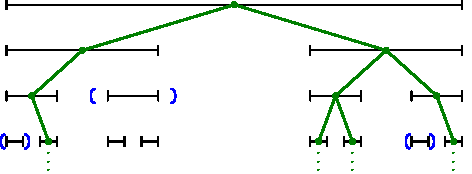
\includegraphics{Figures/CantorSet.pdf}
			\caption{$T$ embedded into the Cantor set. The blue intervals are $\U$.}
		\end{figure}
	
		Because there are no infinite paths in $T$, every infinite binary sequence $\ell$ has a smallest initial segment $\sigma$ where it first exits $T$, for which the real number $f(\ell)$ is in $(a_{\sigma},b_{\sigma})$. This shows that $\U$ covers all of $f(2^{\N})$, i.e. the Cantor set.\\
		
		Now, Heine-Borel implies that $[0,1]$ is compact, and the Cantor set is closed in $[0,1]$ hence it is compact as well. Thus there must be a finite subcover of the Cantor set among $\U$, represented by some $\sigma_1,\sigma_2,\dots,\sigma_j\in U$. Every $\tau\in T$ must be an initial segment of one of these $\sigma_i$, so $T$ is bounded in depth by $\max\{|\sigma_1|,|\sigma_2|,\dots,|\sigma|_j\}$, and hence finite.
	\end{proof}\\
	
	These results suggest the idea that $\WKL$ is the ``combinatorial core'' of compactness, one of the many insights to come out of reverse mathematics. But the question remains: is $\sf{WKL}$ actually weaker than $\KL$ over $\RCA$? 
	
	\newpage
	
	
	
	
	\section{Separation of Problems}
	
	The goal for this section is to prove that $\WKL$ does not prove $\KL$, but we will approach the question more generally: given two problems $\sf{A}$ and $\sf{B}$, how can we prove that $\sf{A}\centernot\implies \sf{B}$? We do it by building a model of $\sf{A}$ in which $\sf{B}$ does not hold. If there is such a model, then that immediately precludes any proof of $\sf{A}\implies \sf{B}$.\\
	
	We've already implicitly used this idea in a simple form when showing that $\RCA$ does not prove the existence of any non-computable set. Similarly, by again working with the $\SS=\Delta_1$ model of $\RCA$, we can show that $\WKL$ is stronger than $\RCA$:\\
	
	\noindent \textbf{Theorem 3.1:} $\RCA\centernot\implies \WKL$.
	\begin{proof}
		In this model, we can construct a binary tree $T$ in $S$ for which there is no path in $S$. In particular, we will ensure that the path is not computable by making the $e$th element of all paths differ from $\Phi_e(e)$: define $T$ by 
		$$
		\sigma \in T \iff (\forall e < |\sigma|):\; \neg\big(\Phi_e(e)[|\sigma|]\downarrow \, \^ \;\, \sigma(e) = \Phi_e(e)\big).
		$$
		That is, $T$ severs a path at the depth when it first detects that $\sigma(e)=\Phi_e(e)$ for any $e$ where $\Phi_e(e)$ halts, and it eventually detects all such discrepancies. Thus, any infinite path (there are many) must disagree with all computable functions, and hence is non-computable.
	\end{proof}\\
	
	Note the difference in strength between $\KL$ and $\sf{WKL}$ here: from the perspective of $\ACA$, as shown in the previous section, there exists a computable tree $T\subseteq \N^{\N}$ whose only path computes $\emptyset'$. In contrast, among \textit{binary} trees $T\subseteq 2^{\N}$, we can force all paths to be non-computable but cannot hit any particular complexity. We could say that $\KL$ \textit{avoids} solutions below $\emptyset'$, whereas $\sf{WKL}$ only avoids (as far as we know) solutions equivalent to $\emptyset$. These are examples of \textit{strength} properties. To separate $\sf{WKL}$ from $\KL$, we will show that $\sf{WKL}$ holds some \textit{weakness} property.\\
	
	Showing that a problem is not provable in $\RCA$ is a convenient case because $\RCA$ has a standard model that we already understand well. But what does a model of $\WKL$ look like? Here, there is not a simple choice for $\SS$ we can just use---we have to make one ourselves. This section will be about the process of model construction and the many tools one can use during that process.
	
	% \newpage
	
	\subsection{Methods of Model-building}
	
	Suppose that we want to construct a model of $\sf{B}\^\neg \sf{A}$, where $\sf{A},\sf{B}$ are two principles between $\RCA$ and $\ACA$. 
	
	% Let $\CC(X)$ denote the cone below $X$, i.e. $\{Z:Z\leq_T X\}$. We'll build $\SS$ in stages $$\CC(\emptyset)\subset \CC(X_1)\subset \CC(X_2)\subset \dots$$
	% and then take 
	% $$
	% \SS := \bigcup_{i\in\N} \CC(X_i).
	% $$
	% To choose $X_i$ 
	
	To construct a model of $\sf{B}$ is fairly simple: you just keep adding solutions to $\sf{B}$ instances until (after $\N$-many steps) everything has a solution. Define sets $Z_0\leq_T Z_1 \leq_T \dots$ inductively as follows: first, let $Z_0=\emptyset$. To define $Z_j$ for $j\geq 1$, let 
	$$X := \text{ the $e_j$th set computed by $Z_{n_j}$}$$
	where $j\mapsto (e_j,n_j)$ is an ordering of $\N\times \N$ such that $n_j<j$ (so that $Z_j$ is not defined referencing itself). If this $X$ is a $\sf{B}$-instance without a $Z_{j-1}$-computable solution, choose a solution $Y$ and let
	$$
	Z_j := Z_{j-1} \oplus Y.
	$$
	Otherwise we let $Z_j=Z_{j-1}$. Finally, define $\SS$ to be the Turing ideal generated by the sets $Z_j$.
	
	For every $\sf{B}$-instance $X\in \SS$, there is a finite stage $n$ in which $X$ is first computable from $Z_n$, and $X$ is the $e$th set computable from $Z_n$ for some $e$, so there must be a stage $j>n$ for which $(e_j,n_j)=(e,n)$ and so a solution to $X$ is added (or already exists). \\
	
	The difficulty is not in modeling $\sf{B}$, but in \textit{not} modeling $\sf{A}$. It suffices to pick a particular $\sf{A}$-instance and deliberately avoid adding any of its solutions to $\SS$ at any stage. In the case of $\sf{A}=\KL$, for example, we might avoid adding $\emptyset'$. But moreover, one also has to avoid adding sets which compute $\emptyset'$, and instances whose only solutions compute $\emptyset'$, and so on. Thus, we look for a sharp dividing line between sets we must add (e.g. $\emptyset$) and sets we don't want to add (e.g. $\emptyset'$) for which we can keep the construction on the right side of the line.\\
	
	% Now, we'll need to repeatedly add solutions to instances of $\sf{B}$, thus we need some way of selecting a particular solution for each instance. Let 
	% $$L:2^{\N}\to 2^{\N}$$
	% map each instance of $\sf{B}$ to a solution of that instance (and for all other $X$ assume $L(X)=\emptyset$). Given a choice of $L$, we can define $\SS$ as the minimal collection of sets which includes $\Delta_1$ and is closed under $L$ and $\Delta_1$-comprehension. 
	
	% This $\SS$ is a model of $\sf{B}$, but possibly of $\sf{A}$ as well. To prevent this, we need to choose a solution-finding map $L$ with special properties.
	
	
	% We begin with a collection of sets $S_0=\Delta_1$. If $\sf{B}$ is stronger than $\RCA$, then $S_0$ will contain $\sf{B}$-instances for which it has no solutions, so we must expand to a larger Turing ideal $S_1\supset S_0$ which solves all the $\sf{B}$-instances in $S_0$. But now $S_1$ may have unsolved $\sf{B}$-instances, so we go on:
	% $$
	% S_0 \subset S_1 \subset S_2\subset \dots 
	% $$
	% and finally we cap our model off by taking the union
	% $$
	% \SS := \bigcup_{j\in \N} S_j.
	% $$
	% Now we have a model of $\sf{B}$. But while we build this model, we also have to be careful to avoid accidentally making $\SS$ a model of $\sf{A}$ as well. 
	
	
	% But this actually entails avoiding many sets: in particular,
	% \begin{align*}
		%     E_1 &= \{X: \text{ all $\sf{B}$-solutions to $X$ compute $\emptyset'$}\}\\
		%     E_2 &= \{X: \text{ all $\sf{B}$-solutions to $X$ compute something in $E_1$}\}\\
		%     E_3 &= \{X: \text{ all $\sf{B}$-solutions to $X$ compute something in $E_2$}\}\\
		%     \vdots &\;\;\;\;\;\;\;\;\vdots 
		% \end{align*}
	% Thus, we need some way to track the ``complexity'' of solutions that we add to $\SS$, and keep this complexity low.\\
	
	\noindent \textbf{Definition (Preservation and Avoidance)}: Let $\QQ$ be some collection of sets that is downward-closed under $\leq_T$ (but not necessarily a Turing ideal). We say that $\sf{B}$ \textit{preserves} $\QQ$ if for every $Z\in \QQ$ and every $\sf{B}$-instance $X\leq_T Z$, there is a solution $Y$ such that $Y\oplus Z\in \QQ$.
	
	If $\QQ$ is upward-closed under $\leq_T$ and $\sf{B}$ preserves $\overline{\QQ}$, then we say $\sf{B}$ \textit{avoids} $\QQ$.\\
	
	\begin{figure}[h]
		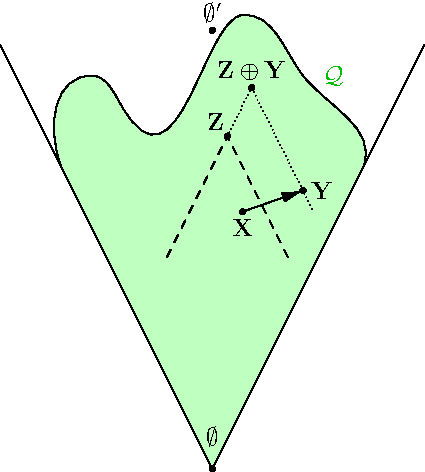
\includegraphics{Figures/Preservation.pdf}
		\caption{$\QQ$-preservation inside the order $\leq_T$. Here, $\QQ$ separates $\emptyset$ from $\emptyset'$.}
	\end{figure}
	
	Clearly, if we find a suitable $\QQ$ and prove that $\sf{B}$ preserves $\QQ$, then a model can be constructed as above while keeping $Z_0,Z_1,Z_2,\dots \in \QQ$, and hence $\SS\subset \QQ$, since by construction every set in $\SS$ is computable from some $Z_j$. 
	
	Now the question becomes choosing a suitable class as $\QQ$. Below are some key examples of $\QQ$ commonly used in preservation and avoidance arguments:
	
	\begin{itemize}
		\item \textbf{Cone Avoidance}: Let $\QQ$ be the ``cone above'' some non-computable set $C$, i.e.
		$$
		\QQ := \{A:  C\leq_T A\}.
		$$
		In this case, if $\sf{B}$ avoids $\QQ$ for all $C$, we say that $\sf{B}$ \textit{admits cone avoidance}. \\
		
		\item \textbf{Low Degree}: Let $\QQ$ be the collection of \textit{low} sets, i.e.
		$$
		\QQ := \{A: A'\equiv_T \emptyset'\}.
		$$
		If $\sf{B}$ preserves $\QQ$, we say that $\sf{B}$ \textit{admits low solutions}.
		
		\noindent There is a similar notion of \textit{low}$_n$ for each $n\in\N$, where $\QQ$ is defined
		$$
		\QQ := \{A: A^{(n)}\equiv_T \emptyset^{(n)}\}.
		$$
		\item \textbf{Hyperimmune-free}: A function $f$ is said to be \textit{hyperimmune} if it is not dominated (i.e. bounded above except at finitely-many values) by any computable function. 
		
		A set is \textit{hyperimmune-free} if it does not compute any hyperimmune function. Being hyperimmune-free is clearly downward-closed under $\leq_T$. If $\sf{B}$ preserves
		$$
		\QQ := \{A: A\text{ is hyperimmune-free}\},
		$$
		we say that $\sf{B}$ \textit{admits hyperimmune-free solutions}.\\
		
		\item \textbf{PA Degree}: $A$ is of \textit{PA degree} if every computable tree $T\subseteq 2^{\N}$ has an $A$-computable path\footnote{The name ``PA degree" comes from the fact that a set $A$ has PA degree if and only if it can compute a complete, consistent extension of Peano Arithmetic. Another equivalent condition is that $A$ can compute a function which can accurately tell \textit{which} of two algorithms halts, given that at least one does.}. From our discussions of $\KL$ and $\sf{WKL}$ so far, it follows that $\emptyset$ does not have PA degree, but $\emptyset'$ does. If $\sf{B}$ avoids
		$$
		\QQ := \{A: A \text{ has PA degree}\},
		$$
		we say that $\sf{B}$ \textit{admits PA avoidance}. 
	\end{itemize}
	
	Note that all four of these classes $\QQ$ separate $\emptyset$ from $\emptyset'$ (choosing $C=\emptyset'$ in the case of cone avoidance). In general, one can relativize each one to separate other pairs of sets.
	
	To make a model of $\WKL$ and not $\KL$, it will suffice to show that $\sf{WKL}$ has any of the above four properties. In fact, we will show all of them except PA avoidance, which $\sf{WKL}$ does not admit.
	
	% \newpage
	
	\subsection{Forcing and its Uses}
	
	To show any $\QQ$-preservation for $\sf{WKL}$ entails constructing a path $Y$ through each $Z$-computable binary tree such that $Y\oplus Z \in \QQ$. To make this and similar constructions easier to follow, we'll use a system of bookkeeping called \textit{forcing}.\\
	
	Forcing is a method of specifying an object (typically a subset of $\N$), which we call $\mathtt{G}$, through a series of approximations. The construction follows a descending path through a partially-ordered collection of \textit{conditions}, denoted $P$. In each stage, the condition $p$ is \textit{extended} to some $p^*\leq p$ (the extension is considered \textit{lower} in the order because it allows a smaller space for possible sets $\mathtt{G}$). 
	
	To instantiate a notion of forcing, then, requires a partially-ordered set $(P,\leq)$, and an order-preserving interpretation of each $p\in P$ as a formula. We also require that $P$ enjoy the ``saturation" property that every descending chain of conditions is satisfied by some $\tt{G}$. 
	
	Before explaining how to use forcing to construct sets with specific desirable properties, let's see a couple of examples of different notions of forcing, each with its own interpretation of $P$:\\
	
	\textbf{Cohen Forcing}: 
	\begin{itemize}
		\item $P = 2^{\N}$, ordered by $p^*\leq p := p^*\succeq p$.
		\item The condition $p$ is interpreted as $p\prec \mathtt{G}$.
	\end{itemize}
	
	\textbf{Jockusch-Soare Forcing}: 
	\begin{itemize} 
		\item $P$ is the set of infinite \textit{computable} sub-trees of $2^{\N}$, ordered by $p^*\leq p := p^*\subseteq p$.
		\item The condition $p$ is interpreted as $\mathtt{G}\in [\, p \,]$, i.e. $\tt{G}$ is a path in $p$.
		\item Unlike the other two forcing notions here, it is not immediately clear that a descending sequence of Jockusch-Soare conditions is satisfied (i.e. a descending sequence of trees has a common path). But this actually follows from the compactness of $[\, 2^{\N}\,]$: each $[\,p\,]$ is a closed (and thus compact) subset of $[\,2^{\N}\,]$, and a descending sequence of compact sets always has a nonempty intersection. 
	\end{itemize}
	
	\textbf{Mathias Forcing}: 
	\begin{itemize}
		\item $P$ is the set of pairs $(E,R)$, where $E$ is a finite set and $R$ is an infinite set, with $E<R$. The order is $(E^*,R^*)\leq (E,R)$ if $E^*\supseteq E\cup R$ and $R^*\subseteq R$. We think of $R$ as the ``reservoir'' of elements that are available to be added to $E$.
		\item $(E,R)$ is interpreted as $E\subseteq  \mathtt{G}\subseteq E\cup R$.
	\end{itemize} 
	
	\begin{figure}[h]
		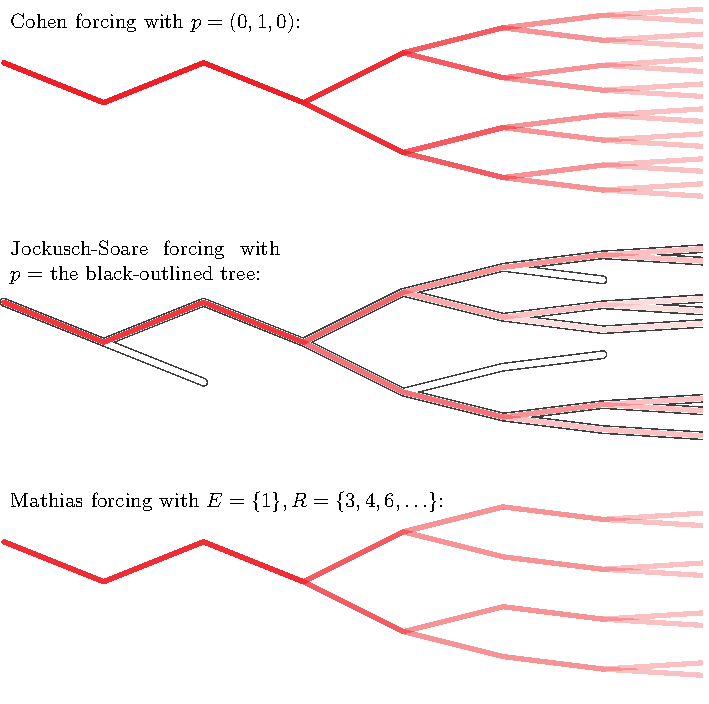
\includegraphics{Figures/ForcingComparison.pdf}
		\caption{The space of sets (visualized as paths in $2^{\N}$) obeying each of three conditions.}
	\end{figure}
	
	Notice that each of these three forcing notions has a different range of formulas that its conditions can articulate. For example, consider the two statements 
	\begin{center}``$\tt{G}$ is infinite'' and ``$\overline{\tt{G}}$ is infinite."\end{center}
	
	In Cohen forcing, there is no condition which could decide either of these for $\tt{G}$, since at any point the undecided elements could all be put in $\tt{G}$ or $\overline{\tt{G}}$. 
	
	In Jockusch-Soare forcing, there are conditions deciding both---in fact, a condition can specify any computable $\tt{G}$ entirely by being a tree with only one path.
	
	In Mathias forcing, there is an asymmetry: no condition can decide whether $\tt{G}$ is infinite because at condition $(E,R)$, $\tt{G}$ could be all of $E\cup R$ (infinite) or only $E$ (finite) or anything in between. However, $(E,R)$ \textit{can} decide that $\overline{\tt{G}}$ is infinite, when $\overline{R}$ is infinite.\\
	
	Though they differ in precision, all three types of conditions are considerably less precise than second-order arithmetic in general. This is what $P$ gives up in exchange for its saturation property. Conditions in $P$ cannot usually enforce the properties that we want in $\tt{G}$, but we can try to get at these properties through infinite descending sequences in $P$, and get a corresponding $\tt{G}$ using saturation.
	
	For example, suppose we are working in the setting of Cohen forcing and we want to produce a $\tt{G}$ which is infinite. As we know, there is no individual condition in $P$ that can guarantee this. However, for each $n\in\N$ there are $p\in P$ which imply $|\mathtt{G}|>n$. In fact, the property $|\mathtt{G}|>n$ is equivalent to obeying at least one condition $p\in P$ which has more than $n$ 1's. If the set of such $p$ is denoted $E_n\subset P$, then we say
	$$
	|\mathtt{G}|>n \iff \mathtt{G} \text{ ``meets" } E_n.
	$$
	To meet a condition-set means to obey at least one of its conditions. We can express $|\mathtt{G}|=\N$ by
	$$
	|\mathtt{G}|=\N  \iff (\forall n): \mathtt{G} \text{ meets } E_n.
	$$
	So if we have a descending sequence of conditions 
	$$
	p_0\geq p_1 \geq p_2 \geq \dots
	$$
	for which $p_n\in E_n$ for each $n$, then the $\mathtt{G}$ approximated by these conditions will meet each $E_n$ and hence be infinite. And it is easy to construct such a sequence, since any condition at all can be extended to one in $E_n$, which is to say that $E_n$ is \textit{dense} in $P$.\\
	
	Of course, this is a very roundabout way of proving that an infinite set exists when one can much more easily name a particular infinite set. But when the desired properties are more complicated, forcing becomes increasingly helpful as a way of organizing the construction of $\tt{G}$.
	
	In general, when we want a set $\tt{G}$ with some particular property $F(\tt{G})$, we express $F$ as a countable list of \textit{dense} condition-sets $D_e\subset P$,
	$$
	(D_0,D_1,D_2,\dots)
	$$
	such that if $\tt{G}$ meets each $D_e$ then $F(\tt{G})$ holds. In all of the cases in this paper, meeting $D_e$ will be equivalent to some definable property of $\tt{G}$, but this is not always the case in general. Using density, we produce a descending sequence of conditions
	$$
	p_0 \geq p_1 \geq p_2 \geq \cdots
	$$
	where $p_e\in D_e$ for each $e$. 
	
	Expressing $F$ as a countable conjunction of dense condition-sets---and proving that they are dense---is the essential piece of any forcing argument.\\
	
	A descending sequence $p_0\geq p_1 \geq \dots$ which meets every dense condition-set in some collection is called \textit{generic}, and a set $\tt{G}$ obeying it is called a generic set. The name ``generic" is quite fitting, since it seems much more unusual to \textit{not} meet a dense set at $\N$-many opportunities than to meet it once. If there exists any sequence of dense condition-sets implying $F$, as described above, then we say that $F(\tt{G})$ holds for any \textit{sufficiently generic} $\tt{G}$. In such a situation, we say that $F$ is \textit{forced}. It may also be that given a certain condition $p$, any sufficiently generic $\tt{G}$ obeying $p$ is forced to hold $F(\tt{G})$, in which case we say $p$ forces $F$.
	
	% The typical construction via forcing looks like this: we want to exhibit a set $\mathtt{G}$ satisfying some desired properties. We express these properties as a countable list of second-order formulas:
	% $$(F_1(X),F_2(X),F_3(X),\dots)$$
	% Then we choose a suitable notion of forcing, $P$, and build a sequence of extensions in $P$:
	% $$
	% p_0\geq p_1\geq p_2\geq \dots
	% $$
	% such that $p_e(X)\Rightarrow F_e(X)$ for each $e$, and conclude by defining $\mathtt{G}$ as a set obeying $p_e(\mathtt{G})$ for all $e$.\\
	% \indent To prove that such a sequence exists, we use induction. For the inductive step, it is sufficient to establish that each $F_e(X)$ is \textit{dense} in $P$, meaning that for any $p\in P$ there is an extension $p^*\leq p$ for which $p^*\imp F_e$. Thus, the difficulty of the argument is in choosing $(F_e)$ and $P$ so that each $F_e$ is dense in $P$, and proving that they are dense.\\
	
	% As an example, Cantor's diagonalization argument can be viewed as a simple case of forcing:\\
	
	% \textbf{Example (Cantor)}: $2^{\N}$ is uncountable.
	% \begin{proof}
		% Given any countable list of sets $$B_1,B_2,B_3,\dots \in 2^{\N},$$ we seek to construct a set $\mathtt{G}$ outside of this list; that is, satisfying $F_e(X) := X\neq B_e$ for all $e\in \N$. Let $P=2^{\N}$, the set of all finite binary strings ordered by $p^*\leq p$ if $p^*\succeq p$ (i.e. $p^*$ contains $p$ as an initial segment). Interpret $p\in P$ as the formula $p\prec \mathtt{G}$, so that each condition $p$ determines membership in $\mathtt{G}$ up to $|p|$.\\
		% \indent Now to show density: for any $p\in P$ of length $\ell$ and $e\in \N$, we can extend $p$ to $p^*$ by appending the opposite of $B_e(\ell+1)$, so that $p^*(\ell+1)\neq B_e(\ell+1)$. Thus, $p^*\imp \mathtt{G}\neq B_e$.
		% \end{proof}\\
	
	% Often, the desired properties may have to be distributed out over the infinite sequence $(F_e)$. For example, using $P=2^{\N}$ as above, properties like ``$\mathtt{G}$ is infinite'' and ``$\mathtt{G}$ is uncomputable'' cannot be guaranteed by any individual condition $p$. But they be broken up as
	% \begin{align*}
		% X \text{ is infinite } &= \bigwedge_{e\geq 1} (|X|>e)\\
		% X \text{ is uncomputable } &= \bigwedge_{e\geq 1} (\Phi_e \neq X)
		% \end{align*}
	% and for any $e$, the formulas $|X|>e$ and $\Phi_e\neq X$ \textit{are} dense in $P$. Also note that, since both lists are dense and countable, one can force both by combining them into a single countable list. In fact, any countable number of separate dense conditions can be stacked like this.\footnote{TO DO: List common decompositions of other useful conditions.}\\
	
	Note that if $F_1,F_2$ are both forced, with the two corresponding sequences of dense condition-sets $(D^1_e)$ and $(D^2_e)$, then $F_1\^F_2$ is also forced, with the sequence
	$$
	(D^1_0,D^2_0,D^1_1,D^2_1,\dots).
	$$
	And naturally the same is true for any countable collection of forced formulas. Thus, conveniently, we may treat every desired property separately.\\
	
	% There are some standard ways to express commonly desired properties in terms of dense sets of conditions. In Cohen forcing, for example, we have the following correspondences:
	% \begin{align*}
		%     |\mathtt{G}|=\N &: D_e := \{p \text{ has more than $e$ 1s}\}\\
		%     \mathtt{G}\nleq_T C &: D_e := \{p(e) \neq \Phi^C_e(e)\}\\
		%     \mathtt{G}\ngeq_T C &: D_e := \{\Phi^p_e\neq \Phi_e^C(e)\}
		% \end{align*}
	% \\
	
	When aiming to construct a set by forcing, the choice of which forcing notion to use is critical. As we've seen, the strengths of each system differ. Cohen forcing is strictly coarser than both Jockusch-Soare and Mathias forcing, and the latter two each have their own areas of high and low precision. If we plan to achieve some property $\ph(\mathtt{G})$ at the $e$th stage of the construction, i.e. to correspond to a dense subset $D_e\subset P$, then $P$ must be coarse enough that no $p\in P$ can ever imply $\neg(\ph(\mathtt{G}))$, yet fine enough that there are $p\in P$ (and densely-many!) implying $\ph(\mathtt{G})$. This is analogous to the choice of a suitable inductive hypothesis: it must be strong enough to prove the inductive step, but weak enough that it can be maintained in each step.
	
	In order to tweak the coarseness of $P$, we will often start with one of the three main forcing notions as a base and then add further restrictions onto $P$. We may even add on new objects to be tracked. For example, we will later see an instance of Mathias forcing which builds two sets at once, each with its own reservoir.
	
	% \newpage
	
	\subsection{The Weakness of \texorpdfstring{$\sf{WKL}$}{WKL}}
	
	% A computable instance of $\WKL$ does not necessarily admit a computable solution. But unlike with $\KL$, there seems to be no way to construct a computable instance of $\WKL$ whose only solution lies in $\Sigma_1$ (we will soon see that no such instance exists). Thus, we may hypothesize that even in the worst case, there will be solutions in some intermediate class between $\Delta_1$ and $\Sigma_1$. We now prove two results of this kind:\\
	
	With the structure of forcing as a guide, we can approach the question of whether $\WKL$ is genuinely weaker than $\ACA$ or not. To do this, it will suffice to show that $\WKL$ admits preservation of some $\QQ$ which separates it from $\emptyset'$, which will allow for the construction of a model of $\WKL$ without $\emptyset'$ in it. We can actually show that $\sf{WKL}$ preserves several of the classes $\QQ$ that we introduced.
	
	In all of these preservation results, we will use a version of Jockusch-Soare forcing, as it is a natural way to constrain objects that we are thinking of as paths in the first place. In each one, note how the fact that $T$ is computably bounded plays an essential role. This is to be expected, given that $\KL$ does not admit any of these weaknesses.\\
	
	\noindent \textbf{Theorem 3.2 ($\sf{WKL}$ Admits Hyperimmune-Free Solutions)}: If $Z$ is hyperimmune-free and $T$ is a $Z$-computable binary tree, there is an infinite path $\ell\in [\,T\,]$ such that $\ell\oplus Z$ is hyperimmune-free; that is, every function computed by $\ell\oplus Z$ is dominated by some computable function.  
	\begin{proof} We'll use Jockusch-Soare forcing with subtrees of $T$.
		
		We want to construct $\mathtt{G}\in [\,T\,]$ such that
		$$
		(\forall e): \Phi_e^{\mathtt{G}\oplus Z} \text{ is computably bounded} 
		$$
		for which it suffices to meet the condition sets
		$$
		D_e := \{p: \ell \in [\,p\,] \imp \Phi_e^{\ell\oplus Z} \text{ is computably-bounded}\}
		$$
		for each $e$. We will show that $D_e$ is dense. \\
		
		Assume otherwise, i.e. that for some tree $p$ there is no extension $p^*$ meeting $D_e$. This implies that there is some depth $d_x$ such that $\Phi_e^{\sigma\oplus Z}(x)[d_x]\downarrow$ for $|\sigma|\geq d_x$; otherwise,
		$$
		p^* := \{\sigma\in p : \Phi_e^{\sigma\oplus Z}(x)[|\sigma|]\uparrow \}
		$$
		would be an infinite $Z$-computable tree whose paths $\ell$ all have $\Phi_e^{\ell\oplus Z}(x)\uparrow$, and thus meet $D_e$.
		
		Moreover, $d_x$ is $Z$-computable as a function of $x$, since $p$ is binary and thus one can explore all depths $d$ until finding one for which $\Phi_e^{\sigma\oplus Z}(x)[d]\downarrow$ for all $|\sigma|=d$. Using this fact, for any given $\ell\in [\,p\,]$ we can construct a $Z$-computable function $g(x)$ that dominates $\Phi_e^{\ell\oplus Z}$:
		$$
		g(x) := \max\{\Phi_e^{\sigma\oplus Z}(x): |\sigma|=d_x\}.
		$$
		And because $Z$ itself is hyperimmune-free, there is also a computable function dominating $g(x)$. Thus, in this case, $p$ already meets $D_e$.
	\end{proof}\\
	
	\noindent \textbf{Theorem 3.3 ($\sf{WKL}$ Admits Cone Avoidance)}: Given a $Z$-computable binary tree $T\subset 2^{\N}$ and a set $C\nleq_T Z$, there is a path $\ell\in [\,T\,]$ for which $\ell\oplus Z$ does not compute $C$. 
	\begin{proof}
		We use Jockusch-Soare forcing, with the modification that all trees in $P$ are subsets of $T$ and are $Z$-computable. The desired condition, not computing $C$, can be expressed as
		$$
		(\forall e): \Phi_e^{\mathtt{G}\oplus Z}\neq C,
		$$
		and $\Phi_e^{\mathtt{G}\oplus Z} \neq C$ is equivalent to meeting the condition set
		$$
		D_e := \{p: \ell \in [\, p \,] \imp \Phi_e^{\ell\oplus Z}\neq C\}.
		$$
		Thus, it suffices to show that $D_e$ is dense in $P$, i.e. that for any tree $p\in P$, there is an extension $p^*\leq p$ (i.e. a subtree) for which $\ell\in [\,p^*\,] \imp \Phi_e^{\ell\oplus Z}\neq C$.\\
		
		Assume for the sake of contradiction that all extensions $p^*\leq p$ in $P$ contain a path $\ell$ with $\Phi_e^{\ell\oplus Z}=C$. We will use this fact to compute $C$ from $Z$, showing a contradiction. The key is that this assumption greatly limits the extent to which the computable functions $\Phi_e^{\sigma\oplus Z}$ can differ from $C$, in two ways:
		\begin{enumerate}[label=(\alph*)]
			\item No $\sigma\in p$ that extends to a path in $p$ has $\Phi^{\sigma\oplus Z}\bot C$; otherwise,
			$$p^*=\{\tau\in p :\tau\succeq \sigma \}$$ 
			would be infinite and meet $D_e$.
			\item For every $x$, there is some depth $d_x$ such that $\Phi^{\sigma\oplus Z}(x)\downarrow$ for all $\sigma\in p$ with $|\sigma|\geq d_x$; otherwise, 
			$$p^*=\{\tau\in p:\Phi^{\tau\oplus Z}(x)[|\tau|]\uparrow \}$$
			would be infinite and also all $\ell\in [\,p^*\,]$ have $\Phi_e^{\ell\oplus Z}(x)\uparrow$, thus $p^*$ would meet $D_e$.
		\end{enumerate}
		Given $d_x$, we can calculate $C(x)$ as follows: let 
		$$D = \{\sigma\in p : |\sigma| = d_x\}.$$
		Because $p$ is a \textit{binary} tree, $D$ is $Z$-computable. We know by (b) that every $\sigma\in D$ has $\Phi^{\sigma\oplus Z}(x)\downarrow$, so we can $Z$-computably split $D$ into 
		$$
		D = A\cup B = \{a_1,a_2,\dots,a_m\}\cup \{b_1,b_2,\dots,b_n\}
		$$
		where $\Phi^{a_j\oplus Z}(x)=0$ and $\Phi^{b_j\oplus Z}(x)=1$. By (a), either $A$ or $B$ (whichever disagrees with $C$) is entirely non-extendable, and hence the depth of its descendants is bounded. Then for each $d'>d$, we can compute from $Z$ the set of nodes of depth $d'$ (again relying on the fact that $p$ is binary) and check which are descended from $A$ versus $B$. For sufficiently large $d'$, only one of the two groups will remain, whence we will have computed $C(x)$ from $Z$.
	\end{proof}\\
	
	From cone avoidance, it also follows as a corollary that $\WKL$ has no minimal model; any non-computable $C$ can be avoided. In other words, like $\RCA$, $\WKL$ does not imply the existence of any particular non-computable set, though it does imply the existence of \textit{some} non-computable set.\\
	
	Next, we'll show that $\sf{WKL}$ also admits low solutions. This argument will be a little bit different from the previous two. It is an example of \textit{effective forcing}, in which a constructed object is made to be $A$-computable (for some $A$) by deciding each of its values at a particular finite stage, and choosing each extension $p^*$ in an $A$-computable way.\\
	
	\noindent \textbf{Theorem 3.4 ($\sf{WKL}$ Admits Low Solutions)}: If $Z\subseteq \N$ is low, then for any $Z$-computable infinite binary tree $T\subset 2^{\N}$, there is an infinite path $\ell\in [\,T\,]$ such that $\ell\oplus Z$ is low, i.e. $(\ell\oplus Z)'\leq_T \emptyset'$.
	
	\begin{proof}
		We'll construct a path $\mathtt{G}\in [\, T\,]$ \textit{and} a $\emptyset'$-computable function $f$ which computes $(\mathtt{G}\oplus Z)'$.\\
		\indent We employ a variant of Jockusch-Soare forcing as follows: 
		\begin{itemize} 
			\item $p\in P$ are of the form $p=(U,\sigma)$, where
			\begin{itemize}
				\item $U$ is an infinite, $Z$-computable subtree of $T$,
				\item $\sigma$ is a finite binary sequence,
				\item $g' \succ \sigma$ for all $g\in [\, U\,]$.
			\end{itemize}
			\item $(U^*,\sigma^*)\leq (U,\sigma)$ if $U^*\subseteq U$ and $\sigma^*\succeq \sigma$.
			\item $(U,\sigma )$ is interpreted as $\mathtt{G}\in [\, U \,]$ and $\sigma \prec f$.
		\end{itemize} 
		The properties of $P$ already guarantee that $f=\ell'$, so the only thing to be forced is that $f$ is total:
		$$
		(\forall e): f(e)\downarrow,
		$$
		and $f(e)\downarrow$ is equivalent to meeting the condition set
		$$
		D_e := \{(U,\sigma): |\sigma| \geq e\}.
		$$
		To ensure that $f$ is $\emptyset'$-computable, we will explicitly construct an extension for $(U,\sigma)$ computably relative to $\emptyset'$, and thus every place of $f$ will be $\emptyset'$-computable.\\
		
		We want an extension $(U^*,\sigma^*)$ such that all $\mathtt{G}\in [\,U^*\,]$ have the same halting behavior on $e$, i.e.
		$$
		\Phi_e^{\mathtt{G}\oplus Z}(e)\downarrow \iff \sigma^*(e),
		$$
		and we need to decide $\sigma^*(e)$ in a $\emptyset'$-computable way. It might be that $U$ already has this property, so we first check if this is the case. We can do this $Z'$-computably (and hence $\emptyset'$-computably, since $Z$ is low): it is equivalent to checking 
		$$
		\Psi(U) := (\exists\, d)(\forall\, \tau\in U): (|\tau|=d) \imp \Phi^{\tau\oplus Z}_e(e)[|\tau|]\downarrow
		$$
		Note that the $\forall$ is bounded because $U$ is a \textit{binary} tree, so $\Psi(U)$ is $\Sigma_1^Z$ and hence $Z'$-computable. If $\Psi(U)$ is true, then $\Phi_e^{\mathtt{G}\oplus Z}(e)\downarrow$ for all $\mathtt{G}\in [\, U \,]$, so we can extend $(U,\sigma)$ to $U^*:=U$ and $\sigma^*(e)=1$. On the other hand, if $\Psi(U)$ is false, the subtree 
		$$E := \{\tau\in U: \Phi^{\tau\oplus Z}_e(e)[|\tau|]\uparrow\}$$
		is infinite and $Z$-computable, so we can take $U^*:=U\cap E$ with $\sigma^*(e)=0$.\\
		
		In summary, we can extend $(U,\sigma)$ in a way depending only on the $\emptyset'$-computable function $\Psi(U)$:
		$$
		(U^*,\sigma^*) := \begin{cases}
			(U,\sigma^{\smallfrown} 1) & \text{if $\Psi(U)$,}\\
			(U \cap E,\sigma^{\smallfrown} 0) & \text{if $\neg\Psi(U)$.}
		\end{cases}
		$$
		In either case, $\Phi^{\mathtt{G}\oplus Z}_e(e)$ has the same halting behavior for all $\mathtt{G}\in [\, U^* \,]$, and it is matched by $\sigma^*(e)$. Since every extension is found $\emptyset'$-computably, $f=(\mathtt{G}\oplus Z)'$ is $\emptyset'$-computable, thus $\mathtt{G}\oplus Z$ is low, as desired.
	\end{proof}\\
	
	With $\sf{WKL}$ shown to admit solutions in several complexity classes not containing $\emptyset'$, we can handily reach this section's goal:\\
	
	\begin{samepage}
		
		\noindent \textbf{Theorem 3.5}: $\WKL\centernot \implies \ACA$.
		\begin{proof}
			This follows from any of the preservation results shown for $\sf{WKL}$, which allow us to build a model of $\WKL$ consisting entirely of $\emptyset'$-cone-avoiding or low or hyperimmune-free sets. The resulting model does not contain $\emptyset'$ as a set, therefore it is not a model of $\KL$ (or $\ACA$).
		\end{proof}\\
		
	\end{samepage}
	
	\begin{figure}[h]
		\begin{tikzcd}
			{\sf{ACA_0}} \\
			\\
			{\sf{WKL_0}} \\
			\\
			{\sf{RCA_0}}
			\arrow[Rightarrow, from=1-1, to=3-1]
			\arrow[Rightarrow, from=3-1, to=5-1]
		\end{tikzcd}
	\end{figure}
	
	Historically, the hierarchy of these three theories has been a focus of reverse mathematics. They are the bottom three of the ``big five" hierarchy, which also includes the stronger theories $\sf{ATR_0}$ and $\Pi^1_1\sf{CA_0}$.\footnote{$\sf{ATR_0}$ stands for Arithmetic Transfinite Recursion. Roughly speaking, it extends $\ACA$ to allow induction and comprehension along any well-order, rather than just $\N$. $\Pi^1_1\sf{CA_0}$ extends comprehension to $\Pi^1_1$ formulas. It is strictly weaker than full second-order arithmetic but stronger than $\sf{ATR_0}$.} The big five are notable because of how many theorems from other areas have been shown equivalent in strength to one of them. 
	
	We have seen already that the completeness of $\R$ is equivalent to $\ACA$ and the compactness of $[0,1]$ is equivalent to $\WKL$. One can actually show that a wide range of results in algebra, analysis, logic, and combinatorics are equivalent to one of these levels. A few key examples are listed below.\footnote{Proofs of all of these equivalences can be found in \cite{simpson}.} 
	
	Note that the language of second-order arithmetic is limited in what it can express; all results below referring to algebraic structures and metric spaces apply only to \textit{countable} structures and \textit{separable} metric spaces, as general uncountable sets are third-order objects and thus cannot be discussed directly in second-order arithmetic. Continuous functions on separable metric spaces are determined by their values on a countable dense set, and thus they can be described as second-order objects.
	
	\begin{itemize}
		\item $\RCA$
		\begin{itemize}
			\item Intermediate Value Theorem
			\item Nested Interval Completeness
			\item Baire Category Theorem 
			\item Existence of algebraic closures 
		\end{itemize}
		\item $\WKL$
		\begin{itemize}
			\item Heine-Borel Theorem (compactness of $[0,1]$)
			\item The Hahn-Banach Theorem 
			\item Riemann integrability of continuous functions
			\item Uniqueness of algebraic closures 
			\item Existence of prime ideals in commutative rings
			\item G\"odel's Completeness and Compactness Theorems
		\end{itemize}
		\item $\ACA$
		\begin{itemize}
			\item Completeness of $\R$
			\item Bolzano-Weierstrass Theorem (sequential compactness of $[0,1]$)
			\item Existence of maximal ideals in commutative rings
			\item Existence of bases for $\Q$-vector spaces
			\item K\"onig's Lemma
		\end{itemize}
	\end{itemize}
	
	In the next section, we will set our reverse-mathematical techniques onto Ramsey's Theorem, a problem from infinitary combinatorics, and investigate its relationship to this hierarchy.
	
	\newpage
	
	\section{Ramsey Theory}
	
	So far, we've developed a nice hierarchy of three naturally-arising theories. We've seen that many statements in second-order arithmetic can be located in one of these three levels. To complicate this picture, we now consider Ramsey's Theorem:\\
	
	\noindent \textbf{Definition (Ramsey's Theorem in degree $n$ for $k$ colors, or $\RT_k^n$):} Given a $k$-coloring of $[\N]^n$ (the size-$n$ subsets of $\N$), i.e. a function $c:[\N]^n\to \{1,2,\dots,k\}$, there exists an infinite set $X$ that is $c$-\textit{homogeneous}, i.e. $c$ is constant on $[X]^n$.\\
	
	In this section, we'll use the methods developed in previous sections---forcing in particular---to determine the precise strength of $\RT^n_k$ relative to the Big Five. This was not known for general $n,k\in \N$ until Liu closed the last remaining case in 2011.
	
	\subsection{\texorpdfstring{$\RT$ over $\RCA$}{RT over RCA}} First, we'll see what can be proven about $\RT^n_k$ over $\RCA$. $\RCA$ does prove some relationships between $\RT^n_k$ for different $n$ and $k$, but we will see that it does not actually prove any $\RT^n_k$ for $n>1$.\\
	
	\noindent \textbf{Lemma 4.1 (Ramsey Theory over $\RCA$):} 
	\begin{enumerate}[label=(\alph*)]
		\item For $k\geq 2$, $\RCA\vdash \RT^1_k$.
		\item For $k\geq 2$, $\RCA\vdash \RT^n_k\iff \RT^n_{k+1}$.
		\item For $n\geq 1$, $\RCA\vdash \RT^{n+1}_k \implies \RT^{n}_k$.
	\end{enumerate}
	\begin{proof} (a): This is essentially the infinitary pigeonhole principle for a fixed number of colors. Given a coloring $c:\N\to \{1,2,\dots,k\}$, the homogeneous sets $$c^{-1}(j):=\{x:c(x)=j\}$$
		are all computable from $c$, thus exist in $\RCA$. One of these sets must be unbounded; if there exist upper bounds $a_j$ on each of these sets so that $c^{-1}(j) < a_j$, then the union of all of them is bounded above by $\max\{a_1,a_2,\dots,a_k\}$, but their union is $\N$, which is unbounded.\\
		
		(b): Given a $(k+1)$-coloring  $c:[\N]^n\to \{1,2,\dots,k+1\}$, we can produce a slightly reduced $k$-coloring by identifying $1$ and $2$:
		$$c^*: A \mapsto \begin{cases}
			1 & c(A)=1\\
			c(A)-1 & c(A) >1
		\end{cases}$$ 
		This $c^*$ clearly $c$-computable, thus it is a function in $\RCA$. Assuming $\RT^n_k$, there exists an infinite $c^*$-homogeneous set $X$. If $X$ is any color other than $1$, then $X$ is also $c$-homogeneous. Otherwise, $c^*(A)\in \{1,2\}$ for $A\in [X]^n$, so $c^*$ is a 2-coloring of $X$. Thus, we can apply $\RT^n_2$ (which clearly follows from $\RT^n_k$) to $c$ on $X$ to get an infinite $c$-homogeneous set. Either case implies $\RT^n_{k+1}$.\\
		
		(c): Given a $k$-coloring $c:[\N]^n\to \{1,2,\dots,k\}$, we have a $k$-coloring 
		$$c^*:[\N]^{n+1}\to\{1,2,\dots,k\} \;\; \text{given by}  \;\; c^*(A)=c(A\setminus \min(A)).$$
		$c^*$ is clearly $c$-computable, thus it is also a function in $\RCA$. Assuming $\RT^{n+1}_k$, there exists a $c^*$-homogeneous set $X$ (say with color $j$). For any size-$n$ subset $B\subset (X\setminus \min(X))$, we have
		$$
		c(B) = c^*(B\cup \{\min(X)\}) = j,
		$$
		thus $X\setminus \min(X)$ is an infinite $c$-homogeneous set of color $j$, implying that $\RT^n_k$ also holds.
	\end{proof}\\
	
	Thus, $\RCA$ proves that the strength of $\RT^n_k$ (for $k\geq 2$) depends only on $n$, and that it is non-decreasing in $n$. As a corollary, $\RCA$ proves that the weakest case of $\RT$ is $\RT^2_2$. The natural question is whether $\RCA$ can actually prove this simplest case, and the answer is: no. To show this, we will give a computable $2$-coloring of $[\N]^2$ with no computable infinite homogeneous set.\\
	
	\newpage 
	
	\noindent \textbf{Theorem 4.2:} $\RCA\centernot\implies \RT^2_2$.
	\begin{proof} We'll describe a coloring algorithm that systematically makes every infinite computable set non-homogeneous. In fact, we can do even better and avoid all infinite c.e. sets. Let
		$$A_e = \{n:\Phi_e(n)\downarrow\}$$
		and denote by $A_e[s]$ the approximation of $A_e$ up to input $s$ and for $s$ steps:
		$$A_{e}[s] := \{n< s : \Phi_e(n)[s]\downarrow\}.$$
		Note that $A_e[s]$ is computable and that $\lim_s A_e[s] = A_e$. We will ensure that if $A_e[s]$ gets sufficiently large, then we eventually color two of its edges oppositely.\\
		
		The construction will proceed in $\N$-many stages: in stage $s$, we decide the colors of edges 
		$$E_s := \{(0,s),(1,s),\dots,(s-1,s)\}.$$
		During stage $s$, for each $e<s$ we compute the set of $x\in A_e[s]$ such that $(x,s)$ is still uncolored. If this set has at least two elements $a,b$, we color their edges oppositely:
		$$
		c((a,s)) = 0, \;\; c((b,s))=1.
		$$
		Otherwise we do nothing and move on. Note that at most 2 edges of $E_s$ can be colored for each $e<s$. At the end of stage $s$, some of $E_s$ may remain uncolored---their colors don't matter.\\
		
		Now to show that the coloring works: if $A_e$ is infinite, then for sufficiently large $s$, 
		$$|A_e[s]|\geq 2e.$$ 
		For such $s$, our coloring is guaranteed to find $a,b\in A_e[s]$ with $(a,s)$ and $(b,s)$ uncolored, since at most $2(e-1)$ edges of $E_s$ can be colored up to this point in stage $s$. And because $A_e$ is infinite, there will be some sufficiently large $s$ which is also in $A_e$, so that $(a,s),(b,s)$ are both edges in $A_e$, and thus $A_e$ is not homogeneous. Thus, we've colored all infinite c.e. sets non-homogeneously.
	\end{proof}\\
	
	This argument focuses on the c.e. sets, but in fact it can be extended to all \textit{limit-computable} sets, i.e. sets $A$ such that
	$$
	A(n) = \lim_m g(n,m)
	$$
	for some computable $g(n,m)$. This requires only a minor change: define $A_e[s]$ as
	$$
	A_e[s] := \{n<s : g_e(n,s)[s]\downarrow = 1\}
	$$
	where $(g_e)$ enumerates the algorithms on two inputs. Define $c$ in the same way relative to $A_e[s]$, and $c$ will color every limit-computable $A$ non-homogeneously by the same argument.
	
	So $\RT^2_2$ implies the existence of non-limit-computable sets, but $\WKL$ \textit{does not}. Because $\sf{WKL}$ admits low solutions, one can build an entirely low model of $\WKL$. Low sets are $\emptyset'$-computable, and hence limit-computable as well,\footnote{In fact, $\emptyset'$-computable and limit-computable are equivalent properties. This is Shoenfield's Limit Lemma.} so we have a model of $\WKL$ whose sets are all limit-computable. Thus, $\WKL$ is not strong enough to prove $\RT^2_2$ (or any other $\RT^n_k$) either!
	
	% Now we'll turn our attention to $\ACA$.
	
	% In $\5$, we needed a coloring that would avoid infinite homogeneous sets of complexity $\Delta_1$. As written, this construction also avoids $\Sigma_1$ sets. But it can be strengthened even further to avoid $\Delta_2$ sets as well, using the characterization of $\Delta_2$ as the limit-computable sets; $\ph_e$ becomes a computable \textit{sequence} of sets, and the approximation $A_e[s]$ becomes an approximation up to time $s$ and input $s$ \textit{of the $s$th set in the sequence}. This establishes that $\WKL\centernot\implies \RT^2_2$. The proof is nearly identical, so I will omit it.\\
	
	
	% \begin{center}
		% \begin{tikzcd}[sep = large]
			% 	{\sf{KL}} && {\sf{ACA_0}} && {\sf{RT}^{\geq 3}_k} \\
			% 	\\
			% 	{\sf{WKL_0}} &&&& {\sf{RT}^2_k} \\
			% 	\\
			% 	&& {\sf{RCA_0}}
			% 	\arrow["\1"', Rightarrow, 2tail reversed, from=1-3, to=1-1]
			% 	\arrow["\4", Rightarrow, 2tail reversed, from=1-3, to=1-5]
			% 	\arrow["\3"', Rightarrow, from=1-3, to=3-1]
			% 	\arrow["\6", Rightarrow, from=1-3, to=3-5]
			% 	\arrow["\7", "\shortmid"{marking}, Rightarrow, 2tail reversed, from=3-1, to=3-5]
			% 	\arrow["\2"', Rightarrow, from=3-1, to=5-3]
			% 	\arrow["\5", Rightarrow, from=3-5, to=5-3]
			% \end{tikzcd}
		% \end{center}
	
	
	\subsection{\texorpdfstring{$\RT$ over $\ACA$}{RT over ACA}}
	
	First, $\ACA$ is strong enough to prove $\RT^n_k$ for all $n$ and $k$:\\
	
	\noindent \textbf{Theorem 4.3}: $\ACA\implies \RT^n_k$. 
	\begin{proof}
		Given a coloring $c:[\N]^n\to \{1,2,\dots,k\}$, we say that a set $X$ is \textit{pre-homogeneous} if the coloring of $n$-edges in $X$ does not depend on their largest element, in the sense that 
		$$
		\forall s\in [X]^{n-1} \text{ and } \, a,b \in X \text{ with } a,b>\max(s), \;\; c(s\cup \{a\}) = c(s\cup \{b\}).
		$$
		Such $c$ and $X$ give rise to a derived coloring 
		$$
		c^*:[X]^{n-1}\to \{1,2,\dots,k\} \;\;\;\; c^*(s) = c(s\cup \{a\}) \;\; \text{where} \;\; a\in X, a>\max(s).
		$$
		Any $c^*$-homogeneous set is also $c$-homogeneous, so if such an $X$ exists for any coloring $c$, then $\RT^{n-1}_k\imp \RT^n_k$. We've shown that $\RT^1_k$ is provable in $\RCA$, so to prove $\RT^n_k$ for every $n$, it suffices to show that an infinite, pre-homogeneous set exists for every coloring.\\
		
		Now given $c$ we'll construct an infinite pre-homogeneous set $\tt{G}$ via a variation of Mathias forcing:
		\begin{itemize}
			\item $p\in P$ are of the form $(E,R)$ where $E$ is finite, $R$ is infinite, and $E<R$.
			\begin{itemize}
				\item Additionally, $E$ must be pre-homogeneous with respect to $c$.
				\item All elements of $R$ must be able to be added to $E$ while maintaining pre-homogeneity.
			\end{itemize}
			\item $(E^*,R^*)\leq (E,R)$ if $E\subseteq E^*\subseteq E\cup R$ and $R^*\subseteq R$.
			\item $(E,R)$ is interpreted as $E\subseteq \mathtt{G}\subseteq E\cup R$.
		\end{itemize}
		We'd like to construct a $\mathtt{G}$ that is infinite, for which it suffices to meet
		$$
		D_e := \{(E,R) : \max{E}>e\}
		$$
		for all $e$. Any such $\tt{G}$ will automatically be pre-homogeneous because of the additional constraints on $P$. We'll show that $D_e$ is dense.\\
		
		Let $(E,R)\in P$ and fix $e$. For each $\sigma:[E]^{n-1}\to \{0,1\}$ (of which there are finitely many) let
		$$
		R_{\sigma} := \{x\in R : (\forall A\in [E]^{n-1}):c(A\cup \{x\}) = \sigma(A)\},
		$$
		so that every element of $R_{\sigma}$ has the same coloring behavior with respect to $E$, and
		$$
		R = \bigcup_{\sigma} R_{\sigma}.
		$$
		$R$ is infinite, so by the pigeonhole principle, at least one of these $R_{\sigma}$ is infinite. Selecting such an $R_{\sigma}$, let $x\in R_{\sigma}$ be its least element above $e$, and choose the extension
		$$
		(E^*,R^*) := (E\cup \{x\},R_{\sigma} \cap (x,\infty))
		$$
		which indeed meets $D_e$, and one can check that $(E^*,R^*)\in P$. Thus, $D_e$ is dense, as desired.
		% Everything done so far is valid in $\RCA$, but to show the existence of pre-homogeneous sets will require the full strength of $\ACA$. We construct $X = \{x_1,x_2,\dots\}$ in steps. Let $Y_k$ be the set of potential values for $x_k$, given $x_1,\dots,x_{k-1}$:
		% $$
		% Y_k = \{y : \, \{x_1,x_2,\dots,x_{k-1},y\} \; \text{is pre-homogeneous}\}.
		% $$
		% Initially, $Y_1=\N$ is infinite. I claim that if $Y_k$ is infinite, then we can choose $x_k$ so that $Y_{k+1}$ is infinite: there are finitely many $n$-edges that $x_{k}$ can make with $x_1,\dots,x_{k-1}$, and finitely many combinations of colors those edges could be, and these colors determine $Y_{k+1}$. Thus, there are finitely many possible sets $Y_{k+1}$, and their union is $Y_{k}$, thus we can choose $x_{k}$ so that $Y_k$ is infinite (by pigeonhole principle). \textit{Checking which one is infinite} is the only part requiring $\ACA$.
	\end{proof}\\
	
	A note on the complexity of this construction: $R_{\sigma}$ is $c$-computable, and testing whether $R_{\sigma}$ is infinite is $c''$-computable, as being infinite is a $\Pi_2$ property. This shows that one can find an infinite pre-homogeneous set that is $c''$-computable. Thus, one can reduce an instance $c$ of $\RT^n_k$ to a $c''$-computable instance of $\RT^{n-1}_k$. To prove $\RT^n_k$, this reduction must be done $n-1$ times, after which $\RT^1_k$ can be computably solved, giving a $c^{(2n-2)}$-computable solution to $c$.\\
	
	We can also show a partial reversal of this result: $\RT^3_2$ (and thus all $\RT^n_k$ for $n\geq 3$) implies $\ACA$. To prove this requires an $A$-computable coloring of triples whose infinite homogeneous sets all compute $A'$:\\
	
	\noindent \textbf{Theorem 4.4 (Jockusch)}: $\RT^3_2 \implies \ACA$.
	\begin{proof}
		Let $A$ be a set. We will describe a $\Delta_1^A$ coloring $c:[\N]^3\to \{0,1\}$ whose only infinite homogeneous sets compute $A'$, and thus show that $A'$ exists for all $A$.\\
		\indent Specifically, consider the following coloring: given a triple $(a,s,t)$ with $a<s<t$, let 
		$$c:(a,s,t)\mapsto \begin{cases}
			0 & \exists (e<a) : \Phi^A_e(e)[s]\uparrow \, \^ \; \Phi^A_e(e)[t]\downarrow\\
			1 & \text{otherwise}
		\end{cases}$$ 
		There are no infinite $c$-homogeneous sets of color 0; if such a set $\{a_1,a_2,\dots\}$ existed, then there would be Turing machines \textit{of index at most} $a_1$ which halt in time-windows $(a_2,a_3],(a_3,a_4],\dots$ but this is impossible because there are only finitely many of these.\\
		\indent Thus, the infinite set $X$ guaranteed by $\RT^3_2$ must have color 1. Let $X=\{a_1,a_2,\dots\}$. Given $X$, we can compute $A'$: to test whether $e\in A'$, take some $a_p>e$ (one exists because $X$ is infinite) and check $\Phi^A_e(e)[a_{p+1}]$. If this doesn't halt then it never will, since $c((a_p,a_q,a_{q+1}))=1$ for $q>p$, hence $\Phi^A_e(e)$ does not halt in $(a_q,a_{q+1}]$ for any $q>p$, and these intervals cover the rest of $\N$.
	\end{proof}\\
	
	This proves that $\RT^3_2$ is equivalent to $\ACA$, and likewise for $\RT^n_k$ with $n\geq 3$, so now $\RT^2_2$ is the only outstanding case. It is unclear how one could encode the halting problem with only a coloring of pairs. Indeed, there turns out to be a genuine difference in strength between $\RT^2_2$ and $\RT^3_2$. To prove this, we will use a forcing argument to show that $\RT^2_2$ admits cone avoidance.\\ 
	
	\newpage 
	
	\noindent \textbf{Theorem 4.5 (Seetapun)}: $\RT^2_2\centernot\implies \ACA$.
	\begin{proof}
		We will prove this by establishing cone avoidance for $\RT^2_2$. That is, we'll show that for any $Z$, if $c:[\N]^2\to\{0,1\}$ is $Z$-computable and $C\nleq_T Z$, then there is an infinite $c$-homogeneous set $\mathtt{G}$ for which $Z\oplus C\nleq_T \mathtt{G}$. We'll assume $Z=\emptyset$ wlog, as it does not affect the argument. 
		
		% Assume for the sake of contradiction that such a $\mathtt{G}$ does not exist. We will construct $\tt{G}$.\\
		
		% \indent Normally, in an argument like this, we would build the set $H$ in stages such that in stage $e$, we guarantee that $\Phi_e^H\neq C$. This is generally difficult to do for Ramsey's Theorem in particular, since the result may not be true for both colors at once; it forces us to choose the correct color at the beginning. \textit{say a little more about this}\\
		% \indent Seetapun's proof maintains flexibility between the two colors: we intend to build \textit{two} sets $\tt{G}_0$ and $\tt{G}_1$, homogeneous of colors $0,1$ respectively, and between them we will ensure that at least one is both infinite and does not compute $C$. We still only need to find one homogeneous set, though, so the outcome we must avoid is that \textit{both} $H_0$ and $H_1$ end up computing $C$, with the Turing Machines of some pair of indices $e_0$ and $e_1$. Indexing our construction by $\N\times\N$, we prevent this outcome in stage $(e_0,e_1)$. \\
		% \indent We will use a notion of Mathias forcing defined as follows: at each stage $(e_0,e_1)$ we have finite conditions $E_0,E_1$ and a ``reservoir'' $R$, representing the set of elements which we may later add to $E_0$ or $E_1$. We say that $(E_0,E_1,R)$ is \textit{valid} if
		% \begin{itemize}
			%     \item $E_0,E_1$ are finite and homogeneous of colors $0$ and $1$.
			%     \item $R\subseteq N_0(E_0)\cap N_1(E_1)$, is infinite, and doesn't compute $C$.
			% \end{itemize}
		% A condition $(E_0^*,E_1^*,R^*)$ extends $(E_0,E_1,R)$ if $E_0\subseteq E_0^*$, $E_1\subseteq E_1^*$, and $R^*\subseteq R$.\\
		
		We can't simply choose a color and begin the construction, since it's possible that there is only an infinite homogeneous set of one color, and it's not apparent which color will work. Instead, we can start constructing \textit{two} homogeneous sets at once, one in each color, and show that \textit{at least one} will have the desired properties. 
		
		Proceeding by contradiction, we'll assume that no such $\tt{G}$ exists. This assumption is necessary to force both sets to be infinite.\\
		
		We construct $\tt{G_0}$ and $\tt{G_1}$ with a variation of 2-fold Mathias forcing defined as follows:
		\begin{itemize}
			\item $p\in P$ are of the form $(E_0,E_1,R)$, where $E_0,E_1$ are finite, $R$ is infinite, and $E_0,E_1<R$.
			\begin{itemize}
				\item Additionally, $E_0$ and $E_1$ must be $c$-homogeneous of colors 0 and 1 respectively.
				\item All elements of $R$ can be added to $E_0$ \textit{or} $E_1$ while maintaining homogeneity.
				\item $R$ must not compute $C$.
			\end{itemize}
			\item $(E_0^*,E_1^*,R^*)\leq (E_0,E_1,R)$ if $E_i\subseteq E_i^*\subseteq E_i\cup R$ for $i\in\{0,1\}$ and $R^*\subseteq R$.
			\item $(E_0,E_1,R)$ is interpreted as $E_i\subseteq \mathtt{G}_i \subseteq E_i \cup R$ for $i\in \{0,1\}$.
		\end{itemize}
		% In the case that $c$ has any infinite homogeneous sets that are \textit{computable}, then clearly such a set does not compute $C$, which is non-computable, which shows cone avoidance. Thus, we can restrict our attention to the other case, in which all infinite $c$-homogeneous sets are non-computable, and use this fact to construct one which does not compute $C$.\\    
		Now we seek to force three properties:
		\begin{enumerate}
			\item $\tt{G_0}$ is infinite.
			\item $\tt{G_1}$ is infinite.
			\item At least one of $\tt{G_0}$ and $\tt{G_1}$ does not compute $C$.
		\end{enumerate}
		We'll show separately that each one is forced.\\
		
		First, some notation: for any set $A$ and color $i\in \{0,1\}$, define the $i$-neighborhood of $A$ as
		$$N_i(A):= \{x : (\forall a\in A): c((a,x)) = i\}.$$
		Note that the conditions on $P$ imply that $R\subseteq N_0(E_0)\cap N_1(E_1)$ for $(E_0,E_1,R)\in P$.\\
		
		(1): It suffices to meet the condition-sets
		$$
		D_e := \{(E_0,E_1,R) : (\max\{E_0\}\geq e)\}
		$$
		for $e\in \N$. If a given $(E_0,E_1,R)$ has no extension meeting $D_e$, then for every $x\geq e$ in $R$,
		$$
		(E_0^*,E_1^*,R^*) := (E_0 \cup \{x\},E_1,R \cap N_0(x))
		$$
		must not be a valid extension, otherwise it would meet $D_e$. This can only be because $R\cap N_0(x)$ is finite for all $x \geq e$ in $R$. But if this is true, then $R\cap N_1(x)$ is infinite for all $x\geq e$ in $R$, which makes it $R$-computable to find an infinite $c$-homogeneous set of color 1: the extension
		$$
		(E_0^*,E_1^*,R^*) := (E_0,E_1 \cup \{x\},R\cap N_1(x))
		$$
		(where $x = \min \{R_{\geq e}\}$) is guaranteed to be valid, so one can repeatedly choose such extensions, resulting in a $\tt{G_1}$ that is $R$-computable and infinite, and hence witnesses cone avoidance. We had assumed that such $\tt{G_1}$ did not exist, so we must now assume that $D_e$ is dense. \\
		
		(2): This follows similarly.
		\\
		
		(3): This property is the most substantive. The only case we must avoid is both $\tt{G_0}$ and $\tt{G_1}$ compute $C$, i.e. for some $e_0,e_1\in \N$, $\Phi^{\tt{G_0}}_{e_0}=\Phi^{\tt{G_1}}_{e_1}=C$. Thus, it suffices to meet the condition-sets
		$$
		D_{(e_0,e_1)} := \{(E_0,E_1,R): (\Phi_{e_0}^{\mathtt{G_0}}\neq C) \vee (\Phi_{e_1}^{\mathtt{G_1}}\neq C) \}
		$$
		for $(e_0,e_1)\in \N^2$. We aim to show that $D_{(e_0,e_1)}$ is dense. Assume otherwise, and that $(E_0,E_1,R)$ is a condition in $P$ with no extensions meeting $D_{(e_0,e_1)}$.\\
		
		% In stage $(e_0,e_1)$, we seek to finitely (and non-trivially, so that our $H_0,H_1$ are sure to be infinite) extend $(E_0,E_1,R)$ to a valid extension $(E_0^*,E_1^*,R^*)$ in such a way that for any $H_0,H_1$ with $E_0^*\subseteq H_0$ and $E_1^*\subseteq H_1$,
		%     $$
		%     \Phi_{e_0}^{H_0} \neq C \;\; \text{or} \;\; \Phi_{e_1}^{H_1}\neq C.
		%     $$
		% Call an extension \textit{forceful} if it guarantees this. If there is \textit{any} such extension, then we can take it (building the model does not have to computable). So assume that none exist.\\
		
		% One way extension could fail is if there are no valid nontrivial extensions $E_0$ (or $E_1$) at all. That would imply that for every $r\in R$, $N_0(r)\cap R$ is finite. But in that case the reservoir can never be depleted by extending $E_1$, so we can find a \textit{computable} infinite $1$-homogeneous set (by always extending to $\min(R)$), which is strictly stronger than not computing $C$. Thus we can assume that all valid reservoirs contain nontrivial extensions of $E_0$ and $E_1$, but that none are forceful.\\
		
		% Our ultimate aim in this proof is to use the non-existence of valid and forceful extensions to compute $C$, yielding contradiction. First, we will show the existence of an infinite and computable set of forceful extensions, then we will find a valid one among them.\\
		
		We define an $i$-\textit{fork} to be a pair of finite $i$-homogeneous sets $(X,Y)$ for which
		$$\exists w< \max(X\cup Y): \;\; \Phi_{e_i}^{E_i\cup X}(w)[\max(X\cup Y)] \downarrow \; \neq \Phi_{e_i}^{E_i\cup Y}(w)[\max(X\cup Y)].$$
		Whereas the property of differing from $C$ is non-computable, the two extensions in an $i$-fork differ from \textit{one another} in a bounded way, which can be verified $R$-computably. Say an $i$-fork is \textit{valid} if 
		$$(E_i\cup X,E_{1-i},R^*) \;\;\; \text{and}\;\;\; (E_i\cup Y,E_{1-i},R^*)$$ are both in $P$, for some $R^*$. If $(X,Y)$ is valid, then one of these two extensions (the one that differs from $C$) must meet $D_{(e_0,e_1)}$, thus it suffices to show that a valid $i$-fork exists. 
		We'll first show the existence of many $i$-forks, and then show there is a valid one among them.\\
		
		\noindent \textbf{Lemma ($\ast$):} Every infinite set $R^*\subseteq R$ which does not compute $C$ must contain an $i$-fork.
		
		\begin{proof}
			Suppose otherwise. We have assumed that no extension meets $D_{(e_0,e_1)}$. This implies that for every $w$ there is some finite $X\subset R^*$ with
			$$
			\Phi_{e_i}^{E_i\cup X}(w)[\max(X)] \downarrow \, = C(w).
			$$
			Otherwise, the extension $(E_0,E_1,R^*)$ would meet $D_{(e_0,e_1)}$, as it implies $\Phi_{e_i}^{\tt{G_i}}(w)$ is either undefined or disagrees with $C(w)$. If, in addition, there are no $i$-forks in $R^*$, then 
			$$
			\Phi_{e_i}^{E_i\cup X}(w)[\max(X)] \in \{\uparrow,C(w)\}
			$$
			for all finite $X\subset R^*$, since no two $X$ can contradict one another. Now we can check all such $X$ until halting, thus computing $C(w)$ from $R^*$, which contradicts the assumption that $C\nleq_T R^*$.
		\end{proof}\\
		
		As an immediate corollary, there are infinitely many $i$-forks (one can take $R^* = R\cap \{x>M\}$ to get an $i$-fork of arbitrarily high minimum). So let $(X_j,Y_j)$ be a \textit{computable} sequence of $0$-forks (one can compute it by repeatedly taking the next largest $0$-fork in some computable ordering):
		$$
		X_0 < Y_0 < X_1 < Y_1 < X_2 < Y_2 < \dots
		$$
		By assumption, all of these $0$-forks are invalid. This is actually a rather strong condition, because it tells us that for any potential reservoir $R^*$, each $X_j\cup Y_j$ contains some $z_j$ for which $N_1(z_j)\cap R^*$ is infinite; otherwise, $R^* \cap_{z\in X_j\cup Y_j} N_0(z)$ would be a valid reservoir for the fork $(X_j,Y_j)$. 
		
		% $N_0(z)$ would be cofinite inside $R$ for all $z\in X_j\cup Y_j$, thus making
		% $$
		% R^* := R\cap \bigg(\bigcap_{z\in X_j\cup Y_j} N_0(z)\bigg)
		% $$
		% an infinite and $R$-computable reservoir for which 
		% $$
		% (E_0\cup X,E_1,R^*), \; (E_0\cup Y,E_1,R^*)\in P.
		% $$
		The goal now is to leverage the invalidity of the $0$-forks to produce a valid $1$-fork within $(z_j)$. We'll first show that such a sequence $z_j$ of sufficient depth $d$ will eventually include a 1-fork. Then, we'll find a reservoir $R^*$ with respect to which all $z\in \{X_j\cup Y_j\}_{j\leq d}$ have edges of only one color. This $R^*$ will serve as reservoir to the 1-fork included in $(z_j)$, hence the 1-fork will be valid.\\
		
		Construct a computable tree $T\subseteq \N^{\N}$ from all sequences $\sigma$ with
		$$
		\sigma(e) \in X_e\cup Y_e
		$$
		such that the immediate parent of $\sigma$ does not contain any 1-forks. $T$ is computably bounded (since $X_e\cup Y_e$ is finite), so if $T$ is infinite then it contains a $C$-cone avoiding path by $\sf{WKL}$ cone avoidance. But by ($\ast$), any infinite non-$C$-computing set necessarily contains 1-forks, so \textit{there can be no such path}, and thus $T$ must be finite. Let its depth be $d$.
		
		\begin{figure}[h]
			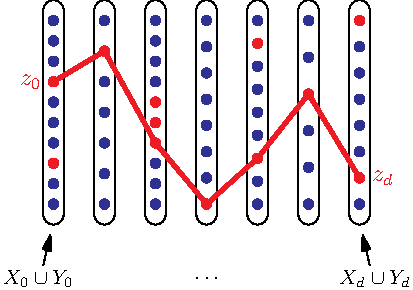
\includegraphics{Figures/SeetapunTree.pdf}
			\caption{The elements of $X_j\cup Y_j$ for $j\leq d$ colored by $\tau$ (blue = 0, red = 1). The sequence $(z_j)$ must contain a valid 1-fork with reservoir $R^*$.}
		\end{figure}
		
		Finally, for each function
		$$
		\tau : \bigcup_{j=0}^d X_j\cup Y_j \to \{0,1\}
		$$
		let
		$$
		R_{\tau} := \{r\in R : (\forall z\in \textrm{Dom}(\tau)): c((z,r)) = \tau(z) \}.
		$$ 
		There are finitely many such $\tau$ since $T$ is finite, and $R_{\tau}$ finitely partitions $R$ into $R$-computable parts. For some $\tau$, $R_{\tau}$ will be infinite: call this $R^*$. Since the $0$-forks $(X_j,Y_j)$ are all invalid, there is a sequence $z_j\in X_j\cup Y_j$ which all have $\tau(z_j) = c(z_j,R^*)=1$. By the definition of $T$, there is a 1-fork among this sequence. This 1-fork is valid, with $R^*$ as its corresponding reservoir.
		% \textit{Alternate approach}: Let $(X,Y)$ be a 0-fork. We assume it to be invalid, which implies that if $R^*$ is any valid reservoir, $N_1(z)\cap R^*$ is infinite for at least one $z\in X\cup Y$ (otherwise $R\cap_{z\in X\cup Y}N_0(z)$ would be infinite). But we can use this to get arbitrarily-long (though not infinite) 1-homogeneous sequences with valid reservoirs. If any of these contain 1-forks, they are guaranteed to be valid, so we must assume there are no 1-forks. Taken together, this is an infinite 1-homogeneous sequence with no 1-forks. If we can construct this sequence in such a way that it avoids computing $C$, then we will derive a contradiction with claim 1.
	\end{proof}\\
	
	This shows that $\RT^2_2$ is strictly weaker than $\RT^3_2$, casting $\RT^2_2$ out of the $\RCA-\WKL-\ACA$ hierarchy, though we haven't yet ruled out the possibility that $\RT^2_2$ lies between $\WKL$ and $\ACA$. Seetapun's proof was published in 1995, but the relationship between $\RT^2_2$ and $\WKL$ was left open until 2011, when Jiayi Liu proved that $\RT^2_2\centernot\implies \sf{WKL}$. Liu showed that $\RT^2_2$ admits PA avoidance by using a Mathias forcing argument.\\
	
	\noindent \textbf{Theorem 4.6 (Liu)}: $\RT^2_2\centernot \implies \sf{WKL}$.
	\begin{proof}
		Omitted. See \cite{dm} or \cite{hirschfeldt} for full proofs of Liu's Theorem.
	\end{proof}\\
	
	With Liu's proof, $\RT^2_2$ could be placed firmly outside of the Big Five hierarchy:
	
	\begin{figure}[h]
		$$\begin{tikzcd}
			\KL && \ACA && {\RT^{\geq 3}_k} \\
			\\
			\sf{WKL} &&&& {\RT^2_k} \\
			\\
			&& \RCA
			\arrow[Rightarrow, 2tail reversed, from=1-1, to=1-3]
			\arrow[Rightarrow, from=1-1, to=3-1]
			\arrow[Rightarrow, 2tail reversed, from=1-3, to=1-5]
			\arrow[Rightarrow, from=1-5, to=3-5]
			\arrow[dashed, no head, from=3-1, to=3-5]
			\arrow[Rightarrow, from=3-1, to=5-3]
			\arrow[Rightarrow, from=3-5, to=5-3]
		\end{tikzcd}$$
		\caption{The full dependency chart between $\RT$ and $\KL$. $\WKL$ and $\RT^2_k$ are independent.}
	\end{figure}
	
	But unlike $\sf{WKL}$, which we find embedded within proofs of all sorts of major theorems throughout mathematics, $\RT^2_2$ is mysteriously not equivalent to any other major theorems. $\RT^2_2$ is its own principle, with its own set of consequences. Much of the work in reverse mathematics in recent decades has been dedicated to studying it.
	
	% But where does $n=2$ actually matter in this proof? One key fact about $n=2$ is that $N_0(x)$ and $N_1(x)$ are complements. In contrast, for $n=3$, 
	
	\subsection{Study of \texorpdfstring{$\RT^2_2$}{RT22}} In this final section, we'll take a look at the world of $\RT^2_2$ and several related coloring principles, and see some longstanding open problems. First, we introduce two new properties a coloring $c:[\N]^2\to \{0,1\}$ can have on a domain $X$:
	
	\begin{itemize}
		% \item \textit{Homogeneous}: $c$ is constant on $[X]^n$.
		\item \textit{Stable}: For $x\in X$, $c$ takes a single value on all but finitely-many edges containing $x$.
		\item \textit{Transitive} For $x<y<z\in X$, $c((x,y))=c((y,z))=q\implies c((x,z))=q$.
	\end{itemize}
	
	Stability and Transitivity turn out to be quite significant classes of colorings. In a sense, they are the only two classes that must be considered; as we will see, if $\RT^2_2$ holds on all stable colorings and all transitive colorings, then it holds in general.\\
	
	$\RT^n_k$ says \textit{any} coloring has an infinite subset on which it is \textit{homogeneous}. This principle can be weakened in several ways. If $\CC$ and $\DD$ are two classes of colorings, let
	$$
	\CC \rightarrowtail \DD \; \; \text{denote} \;\; ``\,\forall c\in \CC, \; \exists \text{ an infinite subset } X\subseteq \N \; \text{ such that } c \in \DD \; \text{on} \; X."
	$$
	Note that $\rightarrowtail$ is transitive. Using this notation, 
	$$
	\RT^2_2 := Any \rightarrowtail Homogeneous.
	$$
	$\RT^2_2$ can be split into several interesting coloring principles based on the coloring classes of stable and transitive, many of which are collected in Figure $\ref{fig:rt22}$.
	
	\begin{figure}[h]
		\begin{center}
			\begin{tikzcd}[sep=large]
				&& {\textit{Homogeneous}} \\
				\\
				\\
				&& {Transitive+Stable} \\
				{\textit{Transitive}} &&&& {\textit{Stable}} \\
				\\
				&& {\textit{Any}}
				\arrow["{\sf{SADS}}"{description}, tail, from=4-3, to=1-3]
				\arrow["{\sf{ADS}}", tail, from=5-1, to=1-3]
				\arrow["{\sf{CADS}}"{description}, tail, from=5-1, to=4-3]
				\arrow["{\sf{SRT}^2_2}"', tail, from=5-5, to=1-3]
				\arrow["{\sf{SEM}}"{description}, tail, from=5-5, to=4-3]
				% \arrow["{\sf{CEM}}"{description}, tail, from=7-3, to=4-3]
				\arrow["{\sf{EM}}", tail, from=7-3, to=5-1]
				\arrow["{\sf{CRT}^2_2}"', tail, from=7-3, to=5-5]
			\end{tikzcd}
		\end{center}
		\caption{A decomposition of the coloring principles below $\RT^2_2$.}
		\label{fig:rt22}
	\end{figure}
	
	\begin{samepage}
		The abbreviations are:
		\begin{itemize}
			\item $\RT$: Ramsey's Theorem.
			\begin{itemize}
				\item $\SRT$ = Stable Ramsey's Theorem.
				\item $\sf{CRT}$ = Cohesive Ramsey's Theorem.
			\end{itemize}
			\item $\mathsf{ADS}$: The Ascending/Descending Sequence Principle.
			\begin{itemize}
				\item For every linear order on $\N$, there is an infinite increasing or decreasing sequence. A linear order can be expressed as a transitive coloring of $[\N]^2$.
				\item $\SADS$ = Stable Ascending/Descending Sequence.
				\item $\sf{CADS}$ = Cohesive Ascending/Descending Sequence.
			\end{itemize}
			\item $\mathsf{EM}$: The Erd\H{o}s-Moser Principle.
			\begin{itemize}
				\item This is sometimes called the ``Tournament Principle," because it can be interpreted as the statement ``for every infinite set of teams, there is an infinite subset on which teams can be linearly ordered by their strength."
				\item $\sf{SEM}$ = Stable Erd\H{o}s-Moser.
			\end{itemize}
			% \item $\mathsf{UCOH}$: The Uniform Coherent Set Principle.
			% \begin{itemize}
				%     \item This is a weaker form of $\COH$, which states that for any collection of functions $$\{f_i:[\NN]\to [k]\}_i$$ there is an infinite set $X\subseteq \NN$ such that all the $f_i$ are stable on $X$.
				%     \item $\sf{UCOH}$ requires the $f_i$ to be uniform in $i$, i.e. that $$c(i,j) := f_i(j)$$ must also be a function in $i,j$. In $\RCA$, this is an important distinction.
				%     \item The distinction matters because the statement that $All\rightarrowtail Stable$ is equivalent to $\UCOH$, taking $c(i,j)=f_i(j)$ to be the coloring, but $\COH$ is strictly stronger.
				% \end{itemize}
		\end{itemize}
	\end{samepage}
	It is known that all of these principles lay in the expanse strictly between $\RCA$ and $\RT^2_2$, though in many cases this is very nontrivial. In terms of their relative strengths, some equivalences can be found by identifying paths in the diagram: for instance,
	$$
	\ADS + \EM \iff \SRT^2_2 + \CRT^2_2 \iff \RT^2_2.
	$$
	But there are also some unexpected implications---for example, we will show that $\ADS \imp \CRT^2_2$. In fact, $\ADS$ proves the \textit{Cohesive Set Principle} ($\COH$), which is a stronger result. 
	
	$\COH$ states that for any sequence of functions $f_i:\N\to \{0,1\}$, there is a set $A$ for which all of the $f_i$ are stable (i.e. converge to 0 or 1) on $A$---we say that $A$ is a \textit{cohesive set} for $(f_i)$. $\CRT^2_2$ follows from a special case of $\COH$ where
	$$f_i(x):= c((i,x))$$
	and, say, $f_i(i):=0$ (the diagonal values do not matter to the cohesiveness of $A$). The essential difference is that $f_i(x)$ must be stable on $A$ for all $i$, whereas $c((i,x))$ only needs to be stable for $i\in A$. \\
	
	\noindent \textbf{Lemma 4.7}: $\ADS \implies \sf{COH}$. 
	\begin{proof}
		% ($\SRT^2_2+\COH\implies \RT^2_2$): Given a (not necessarily stable) coloring $c:[\NN]^2\to \{0,1\}$, let $C$ be the set given by $\COH$ on which 
		% $$
		% f_i : x \mapsto c((i,x))
		% $$
		% stabilizes for all $i$. Then $c$ is a stable coloring of $[C]^2$, thus by $\SRT^2_2$, $C$ contains an infinite $c$-homogeneous set $X\subseteq C\subseteq \NN$.\\
		Given a sequence of functions $f_i:\N\to \{0,1\}$, let $f(x)$ denote the binary sequence
		$$
		f(x) := (f_1(x),f_2(x),f_3(x),\dots).
		$$
		We may assume that $f$ is injective\footnote{In general, we can interleave the sequence $f_i$ with a characteristic functions $\chi_i$ for each $i$, which makes $f$ injective. Proceeding with the proof will yield a set $A$ that is cohesive for both $f_i$ and $\chi_i$, which also serves as a cohesive set for just the $f_i$.}. Between two binary sequences there is a lexicographic order; e.g. $(1,0,0,1,1,\dots) > (1,0,0,1,0,\dots)$. Let $c:[\N]^2\to \{0,1\}$ color pairs based on this ordering:
		$$
		\text{for} \; x<y, \;\; c: (x,y)\mapsto \begin{cases}
			0 & f(x) < f(y) \\
			1 & f(x) > f(y)
		\end{cases}
		$$
		Given that $f(x)\neq f(y)$, the sequences differ at some finite index, so $c$ is computable relative to the functions $f_i$. Then, by $\ADS$ there must exist an infinite ascending (wlog) subsequence
		$$A = \{a_1,a_2,\dots\},$$
		so that 
		$$
		f(a_1) < f(a_2) < f(a_3) < \dots
		$$
		Now we can show (in $\RCA$) that $A$ is a cohesive set for the functions $f_i$: for any $n$, the $n$-tuple
		$$(f_1(a_j),f_2(a_j),\dots,f_n(a_j))$$
		is non-decreasing in $j$, and takes at most $2^n$ values, so it changes at most $2^n$ times. In particular, this implies $\{f_n(a_j)\}_j$ changes between 0 and 1 at most $2^n$ times, and thus is eventually constant. As this is true of all $n$, $A$ is cohesive for the functions $f_i$.
	\end{proof}\\
	
	Thus, as promised, $\RT^2_2$ can be reduced to the two cases of transitive and stable colorings, as
	$$
	\SRT^2_2 + \ADS \implies \SRT^2_2 + \CRT^2_2 \iff \RT^2_2.
	$$
	This decomposition is unique to $n=2$, as the property of transitivity does not make sense for colorings with $n\geq 3$. The decomposition can be used to more easily prove weakness principles for $\RT^2_2$ by proving them for $\SRT^2_2$ and $\ADS$ (or $\COH$), which are often simpler. Both Seetapun's Theorem and Liu's Theorem have ``modernized" proofs along these lines.
	
	\begin{figure}[h]
		$$\begin{tikzcd}[sep=large]
			&& {\RT^2_2} \\
			{\sf{ADS}} &&&& {\SRT^2_2} \\
			\\
			& {\CRT^2_2} & {\sf{SADS}} & {\sf{EM}} \\
			{\sf{CADS}} &&&& {\sf{SEM}} \\
			&& {\sf{RCA_0}}
			\arrow[Rightarrow, from=1-3, to=2-1]
			\arrow[Rightarrow, from=1-3, to=2-5]
			\arrow[Rightarrow, from=1-3, to=4-2]
			\arrow[Rightarrow, from=1-3, to=4-4]
			\arrow[Rightarrow, from=2-1, to=4-2]
			\arrow[Rightarrow, from=2-1, to=4-3]
			\arrow[Rightarrow, from=2-1, to=5-1]
			\arrow[Rightarrow, from=2-5, to=4-3]
			\arrow[Rightarrow, from=2-5, to=5-5]
			\arrow[from=4-2, to=5-1]
			\arrow[Rightarrow, from=4-3, to=6-3]
			\arrow[from=4-4, to=5-5]
			\arrow[Rightarrow, from=5-1, to=6-3]
			\arrow[Rightarrow, from=5-5, to=6-3]
		\end{tikzcd}$$
		\caption{Known dependencies between principles below $\RT^2_2$.}
		\label{fig:last}
	\end{figure}
	
	The presently-known implications among the coloring principles discussed in this section are listed above in Figure \ref{fig:last}.
	
	The single arrows denote implications that are not proven to be strict (i.e. may be equivalences). Two open questions are whether $\sf{SEM}$ is weaker than $\EM$ and whether $\sf{CADS}$ is weaker than $\sf{CRT}^2_2$. Between $\CRT^2_2$, $\SADS$, and $\EM$, five of six non-implications have been proven; the only unproven one is whether $\EM\imp \CRT^2_2$, or more generally whether $\EM\imp \COH$. The precise strength of $\EM$ remains uncertain.
	
	The full state of progress on these and many other questions in reverse mathematics is cataloged and displayed in the \href{https://rmzoo.math.uconn.edu/diagrams/}{Reverse Mathematics Zoo}, though the diagrams there are not up to date.\\
	
	\section*{Acknowledgments}
	
	I would like to thank Professors Maryanthe Malliaris and Denis Hirschfeldt for giving helpful advice and direction during this project. I am especially grateful to my REU mentor Miles Kretschmer for teaching me all that I know about reverse mathematics and providing excellent feedback on dozens of drafts of this paper.
	
	\printbibliography
	
	
\end{document}
